%%____________________________________________________________________________||
\section{Interpretation in Simplified SUSY models with Long-lived Mediators}
\label{sec:LLP}

As an additional interpretation of the results in this search, we investigate a simple extension to the 
simplified supersymmetric model T1qqqq of section~\ref{sec:susy} where the mediating sparticle is ``long-lived''.
In these cases, the final visible decay products may be produced with a non-negligible displacement from the interaction vertex.
To distinguish these models from the that of section~\ref{sec:susy}, we refer to these models as T1qqqqLL.


\subsection{Signal models}
\label{sec:LLP_models}

% TO COVER:
% T1qqqq decay, link to figure from last section: \ref{fig:T1qqqq_feyn}
% The range of lifetimes considered, implications for decay vertex (less than b-lifetime, outside the tracker, outside ECAL, etc)
% Generation of signal samples: Full sim vs. FastSim as for standard SUSY

\clearpage
\subsection{Signal acceptance times efficiency}
\label{sec:sig-accept-contam-LLP}

In Tab. \ref{tab:sig-eff-LLP} the signal efficiency for benchmark mass
points and lifetimes (as \ctau) is summarised.
% Signal efficiency figures across ctau vs mass plane?
%The signal efficiency across
%the whole ($m_{\mathrm{Susy}},m_{\mathrm{LSP}}$) for the simplified
%models used in the analysis is shown in
%Figs.~\ref{fig:T1qqqq_eff}-\ref{fig:T2cc_eff}.

\begin{table}[h!]
    \scriptsize
	\caption{Signal efficiency for T1qqqqLL with different \ctau values.}
    \label{tab:sig-eff-LLP}
    \centering
    \begin{tabular}{ ll }
        \hline \hline
	    \ctau (mm) & Efficiency (total) \\ 
            0.001 & 20.5\% \\
            0.01  & 20.5\% \\
            0.1   & 20.5\% \\
            1     & 20.5\% \\
            10    & 20.5\% \\
            100   & 20.5\% \\
            1000  & 20.5\% \\
        \hline \hline
    \end{tabular}
\end{table}

% Discuss: Variation of Signal Efficiency around B-lifetime ?
% Discuss: Signal contamination of the CRs?  Generally not an issue since no leptons. Sidebands?

\clearpage
\subsection{Systematic uncertainties on signal efficiency times acceptance}
\label{sec:sig-syst-LLP}

The following sources of systematic uncertainty are propagated to the signal
acceptance and shape, according to the recommendations agreed on within the
collaboration. Relative effect on the yields are presented in
Tab.~\ref{tab:sig-systematics-LLP} for some benchmark models.

\begin{itemize}
    \item Luminosity: 2.6\%, taken as correlated across all bins.
    \item Trigger: conservatively, the size of the inefficiency is taken as
        systematic variation where not in the plateau (see Sec.~\ref{sec:triggers}).
    \item MC statistics:  uncorrelated bin-by-bin uncertainty, affecting the
        shape of the signal.
    \item Pileup reweighting: 5.0\% uncertainty on the minimum bias cross section
        (see Sec.~\ref{sec:pileup-reweighting}).
    \item b-tag efficiency: uncertainty on the FullSim and FastSim b-tag scale
        factor is propagated and taken as correlated across the bins.
    \item Lepton efficiency: uncertainty on the lepton scale factors is
        propagated and taken as correlated across the bins.
    \item Jet energy scale: uncertainty on the jet energy corrections is
        propagated and taken as correlated across the bins.
    \item Initial State Radiation (ISR): Reweighting of the $N_{\text{isr}}$
        distribution. The systematic is taken as half the corrections.
\end{itemize}

\begin{table}[h!]
        % TODO CHANGE THIS TABLE
    \scriptsize
    \caption{
        Representative range taken from the $16\%$ and $84\%$ percentiles of the
        uncertainty across the analysis bins for each source of signal
        systematic. Two benchmark point are chosen for each model, corresponding
        to ``compressed'' and ``uncompressed'' scenarios, i.e. with small and
        large mass splitting between the mother particle and the LSP. A third
        benchmark is chosen for T2tt for the $W$ corridor and no
        ``uncompressed'' is chosen for T2cc.
    }
    \label{tab:sig-systematics-LLP}
    \centering
    \begin{tabular}{ ccccccccc }
        \hline \hline
        Model & ($m_{\mathrm{Susy}},m_{\mathrm{LSP}}$) & Luminosity & ISR & JEC & PU & b-tag & Trigger & MC stat. \\ \hline
        \multirow{2}{*}{T1qqqq}
            & (1700,100) & 2.6\% & 2-4\%  & 2-12\% & 6-12\% & 1-1\% & 1-2\% & 14-19\% \\
            & (1000,850) & 2.6\% & 3-14\% & 5-14\% & 9-14\% & 3-7\% & 2-4\% & 6-22\%  \\
        \hline
        \multirow{2}{*}{T1bbbb}
            & (1900,100)  & 2.6\% & 3-9\%  & 4-6\%  & 7-14\% & 7-12\% & 4-5\% & 11-19\% \\
            & (1300,1100) & 2.6\% & 2-11\% & 3-11\% & 5-9\%  & 2-5\%  & 1-3\% & 11-22\% \\
        \hline
        \multirow{2}{*}{T1tttt}
            & (1700,100) & 2.6\% & 2-6\% & 3-15\%  & 2-9\%  & 2-6\% & 2-4\% & 12-24\% \\
            & (950,600)  & 2.6\% & 5-9\% & 12-26\% & 7-13\% & 2-6\% & 3-7\% & 15-30\% \\
        \hline
        \multirow{2}{*}{T2qq (1-fold)}
            & (700,100) & 2.6\% & 2-7\%  & 3-10\% & 6-9\%  & 0-5\% & 1-4\% & 4-22\% \\
            & (400,300) & 2.6\% & 5-22\% & 5-18\% & 9-15\% & 3-5\% & 3-5\% & 6-20\% \\
        \hline
        \multirow{2}{*}{T2qq (8-fold)}
            & (1250,100) & 2.6\% & 2-7\%  & 5-14\% & 5-10\% & 1-1\% & 1-3\% & 12-24\% \\
            & (700,600)  & 2.6\% & 4-17\% & 4-13\% & 9-14\% & 2-5\% & 2-4\% & 6-22\%  \\
        \hline
        \multirow{2}{*}{T2bb}
            & (1000,100) & 2.6\% & 1-7\%  & 4-11\% & 5-9\%  & 1-4\% & 0-3\% & 14-23\% \\
            & (550,450)  & 2.6\% & 4-15\% & 4-15\% & 8-13\% & 3-7\% & 2-3\% & 9-22\%  \\ 
        \hline
        \multirow{2}{*}{T2tt}
            & (1000,50) & 2.6\% & 3-7\%   & 4-14\% & 6-10\%  & 1-5\%  & 1-4\%  & 14-27\% \\
            & (450,200) & 2.6\% & 4-12\%  & 6-15\% & 10-14\% & 4-9\%  & 3-6\%  & 6-19\%  \\
            & (250,150) & 2.6\% & 13-27\% & 8-22\% & 12-25\% & 6-16\% & 6-17\% & 10-23\% \\
        \hline
        \multirow{1}{*}{T2cc}
            & (500,480) & 2.6\% & 4-18\% & 5-13\% & 5-12\% & 1-4\% & 2-4\% & 6-19\% \\
        \hline \hline
    \end{tabular}
\end{table}

\clearpage
\subsection{Exclusion limits}
\label{sec:LLP_results}

\begin{table*}[!t]
  \topcaption{Expected ($\mu_{\text{exp}}$) and observed 
    ($\mu_{\text{obs}}$) upper limits on the production cross section, 
    expressed in terms of the signal strength parameter, obtained using
    both the nominal and simplified binning schema. 
  }
  \label{tab:aggr_limits}
  \centering
  \begin{tabular}{ llccccc }
    \hline
    \multicolumn{2}{c}{Benchmark models}    & \multicolumn{2}{c}{Nominal}
                                            & 
                                            & \multicolumn{2}{c}{Simplified}             \\ [0.3ex]
    \cline{3-4}
    \cline{6-7}
   %\multicolumn{2}{c}{$(m_{\text{SUSY}}, m_{\mathrm{LSP}})$ [\GeVns{}]} 
                                              \ctau [mm] 
                                            & $(m_{\text{SUSY}}, m_{\mathrm{LSP}})$ [\GeVns{}]
                                            & $\mu_{\text{exp}}$
                                            & $\mu_{\text{obs}}$
                                            & 
                                            & $\mu_{\text{exp}}$
                                            & $\mu_{\text{obs}}$                         \\ [0.3ex]
    \hline
    \multirow{2}{*}{0.001}  & (1800, 200)   & 0.81 & 1.58 &  & 1.22  & 1.53 \\
                            & (1000, 900)   & 0.95 & 1.21 &  & 2.23  & 2.28 \\ [0.5ex]
    \multirow{2}{*}{1}      & (1800, 200)   & 0.36 & 0.66 &  & 0.47  & 0.44 \\
                            & (1200, 1100)  & 6.72 & 2.99 &  & 26.13 & 16.76 \\ [0.5ex]
    \multirow{2}{*}{100000} & (1000, 200)   & 0.95 & 1.33 &  & 1.88 & 2.32 \\
                            & (1000, 900)   & 0.95 & 0.73 &  & 1.90 & 1.47 \\ 
    \hline
  \end{tabular}
\end{table*}

%Summary exclusion plots according to this categorisation are presented in
%Fig.~\ref{fig:summary-excl-plots}.

\newpage
\begin{figure}[h!]
    \begin{center}
        \subfigure[T1qqqqLL (\ctau = 0.001~mm): Upper limit on the cross section in the mass plane]{
            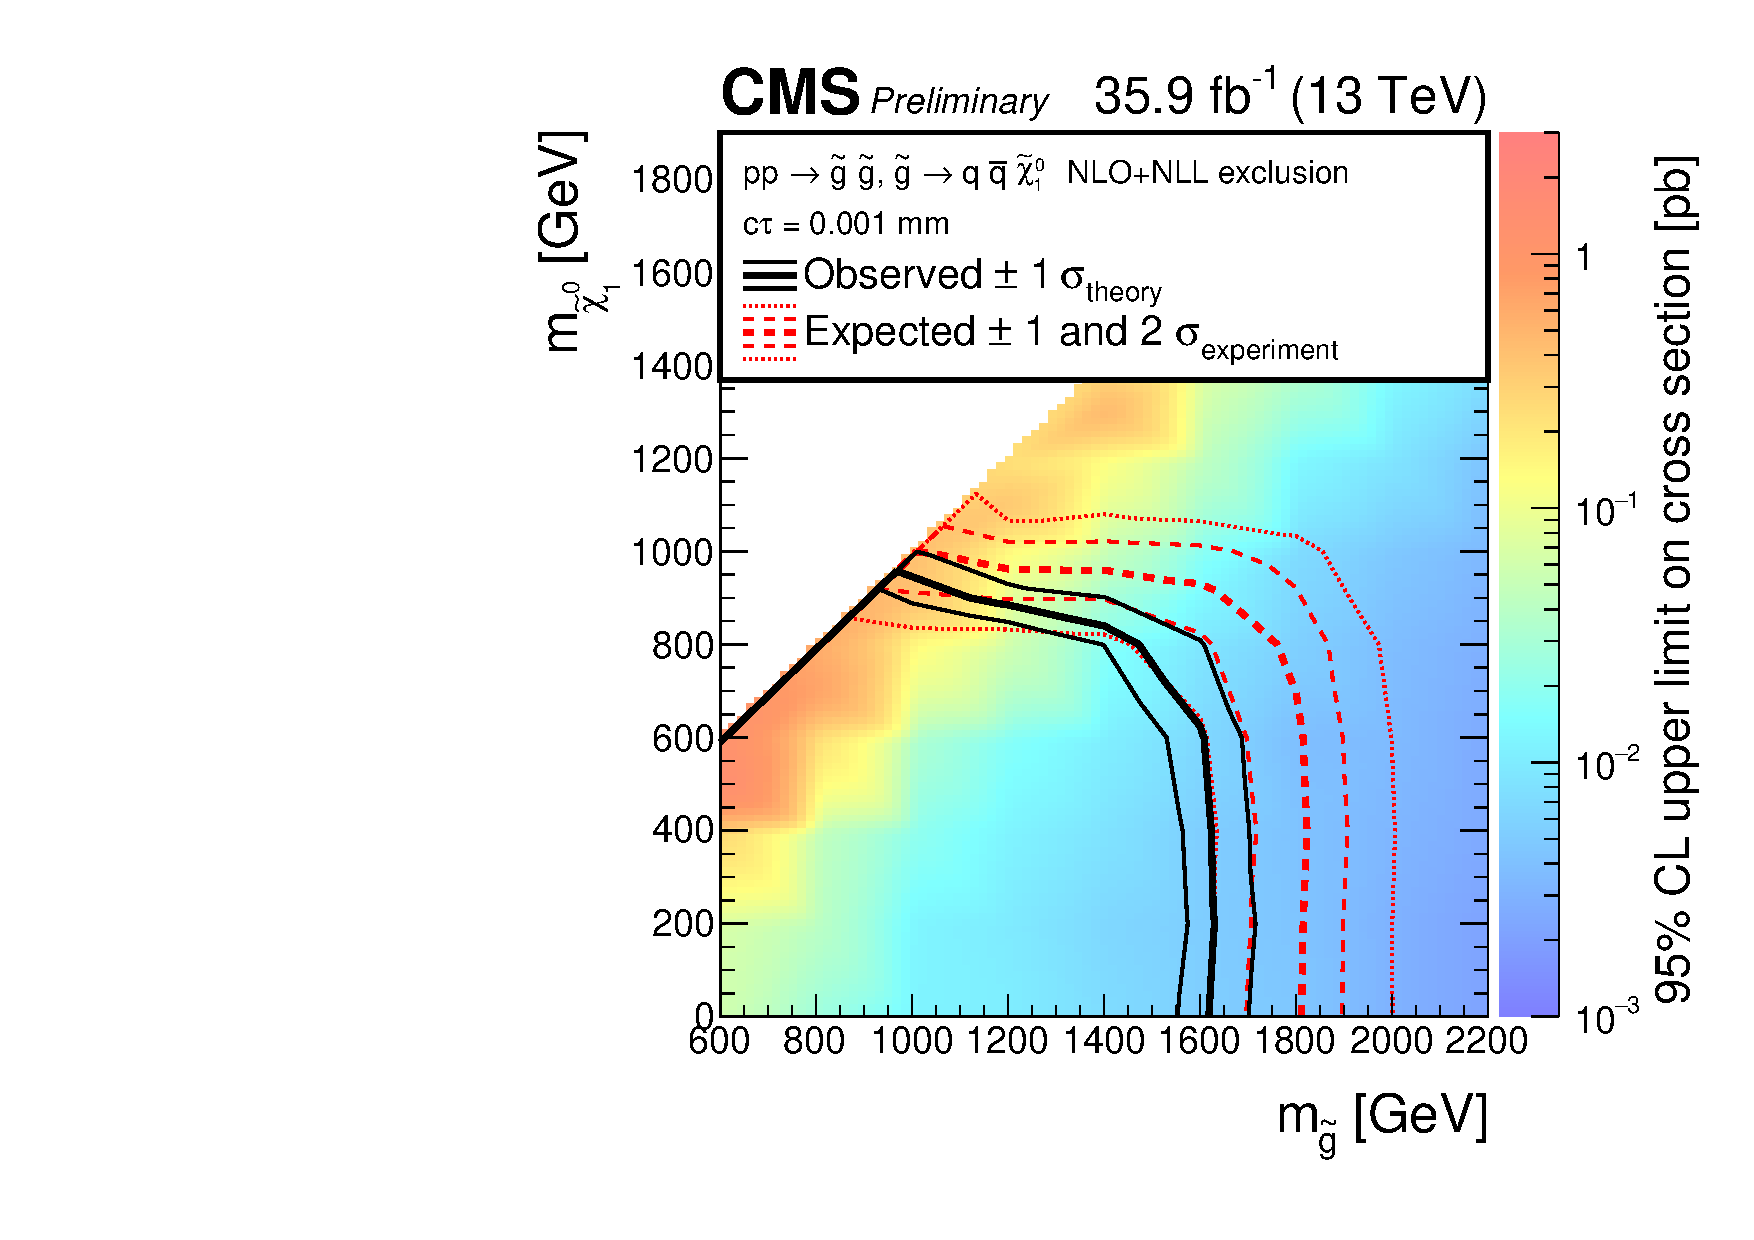
\includegraphics[width=0.6\textwidth]{figures/LLPResults/T1qqqqLL_ctau-0p001_XSEC}
            \label{fig:T1qqqqLL_excl}
        } \\
        \subfigure[T1qqqqLL (\ctau = 0.001~mm): $\epsilon_{sig}$]{
            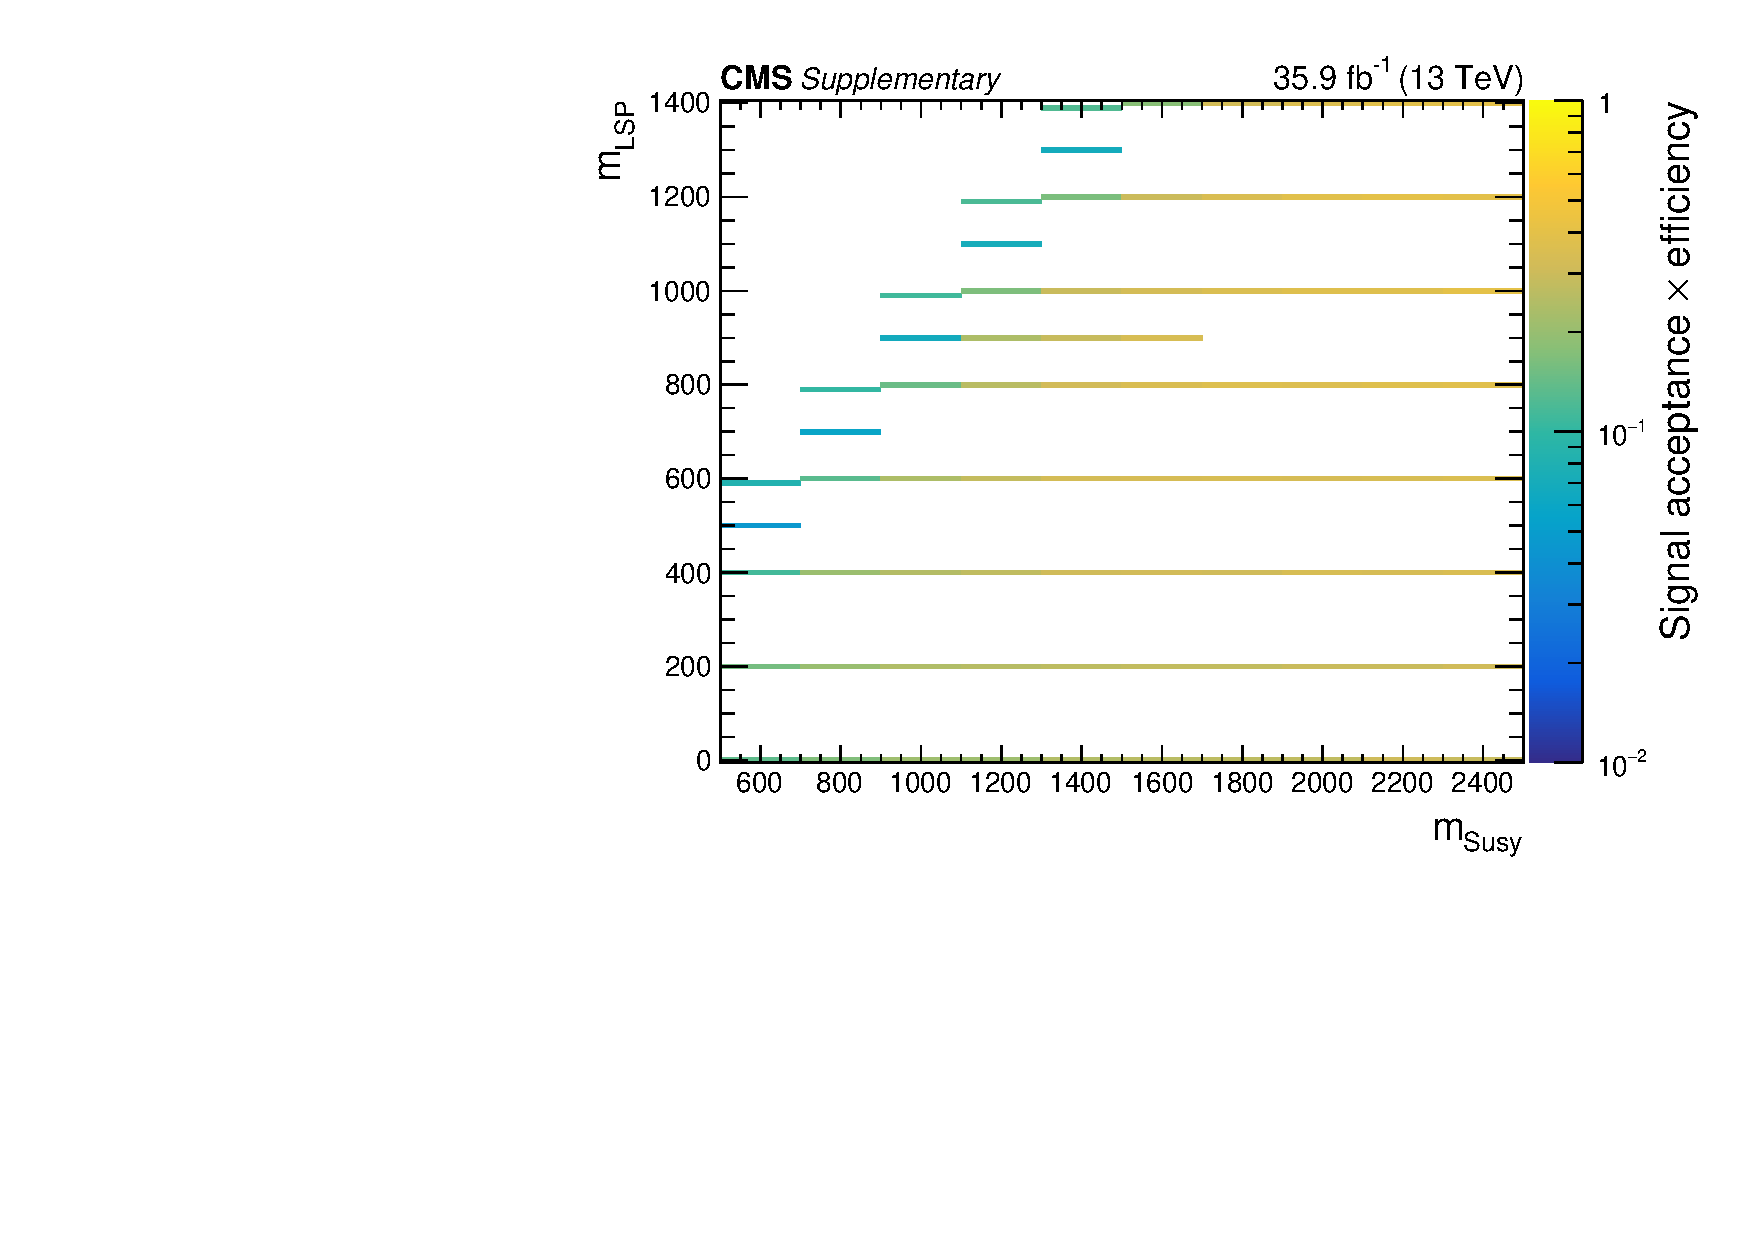
\includegraphics[width=0.45\textwidth]{figures/LLPResults/T1qqqqLL_ctau-0p001_effs}
            \label{fig:T1qqqqLL_eff}
        } ~~
        \subfigure[T1qqqqLL (\ctau = 0.001~mm): Most sensitive categories]{
            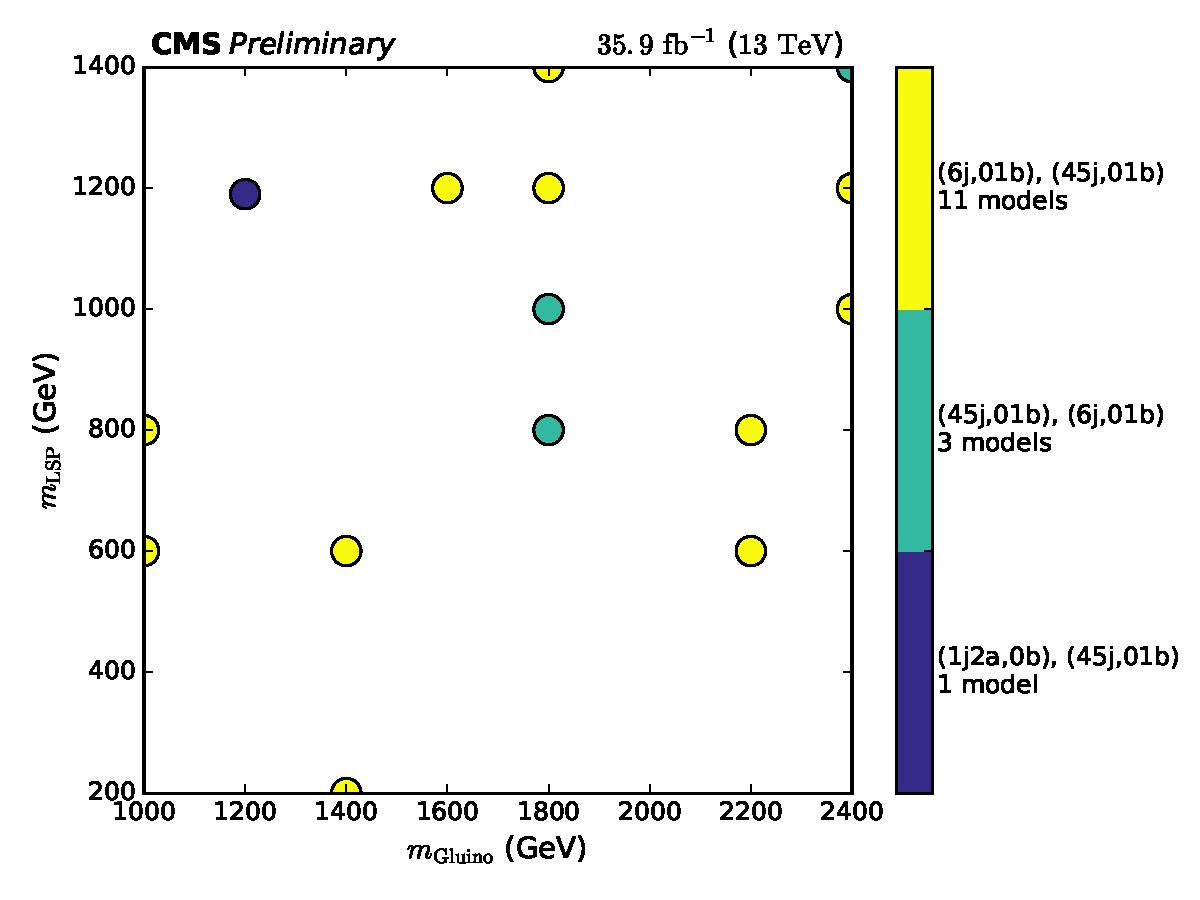
\includegraphics[width=0.45\textwidth]{figures/LLPResults/T1qqqqLL_ctau-0p001_bitMap}
            \label{fig:T1qqqqLL_bitMap}
        } \\
        %\subfigure[T1qqqqLL (\ctau = 1~mm): Significance scan]{
        %    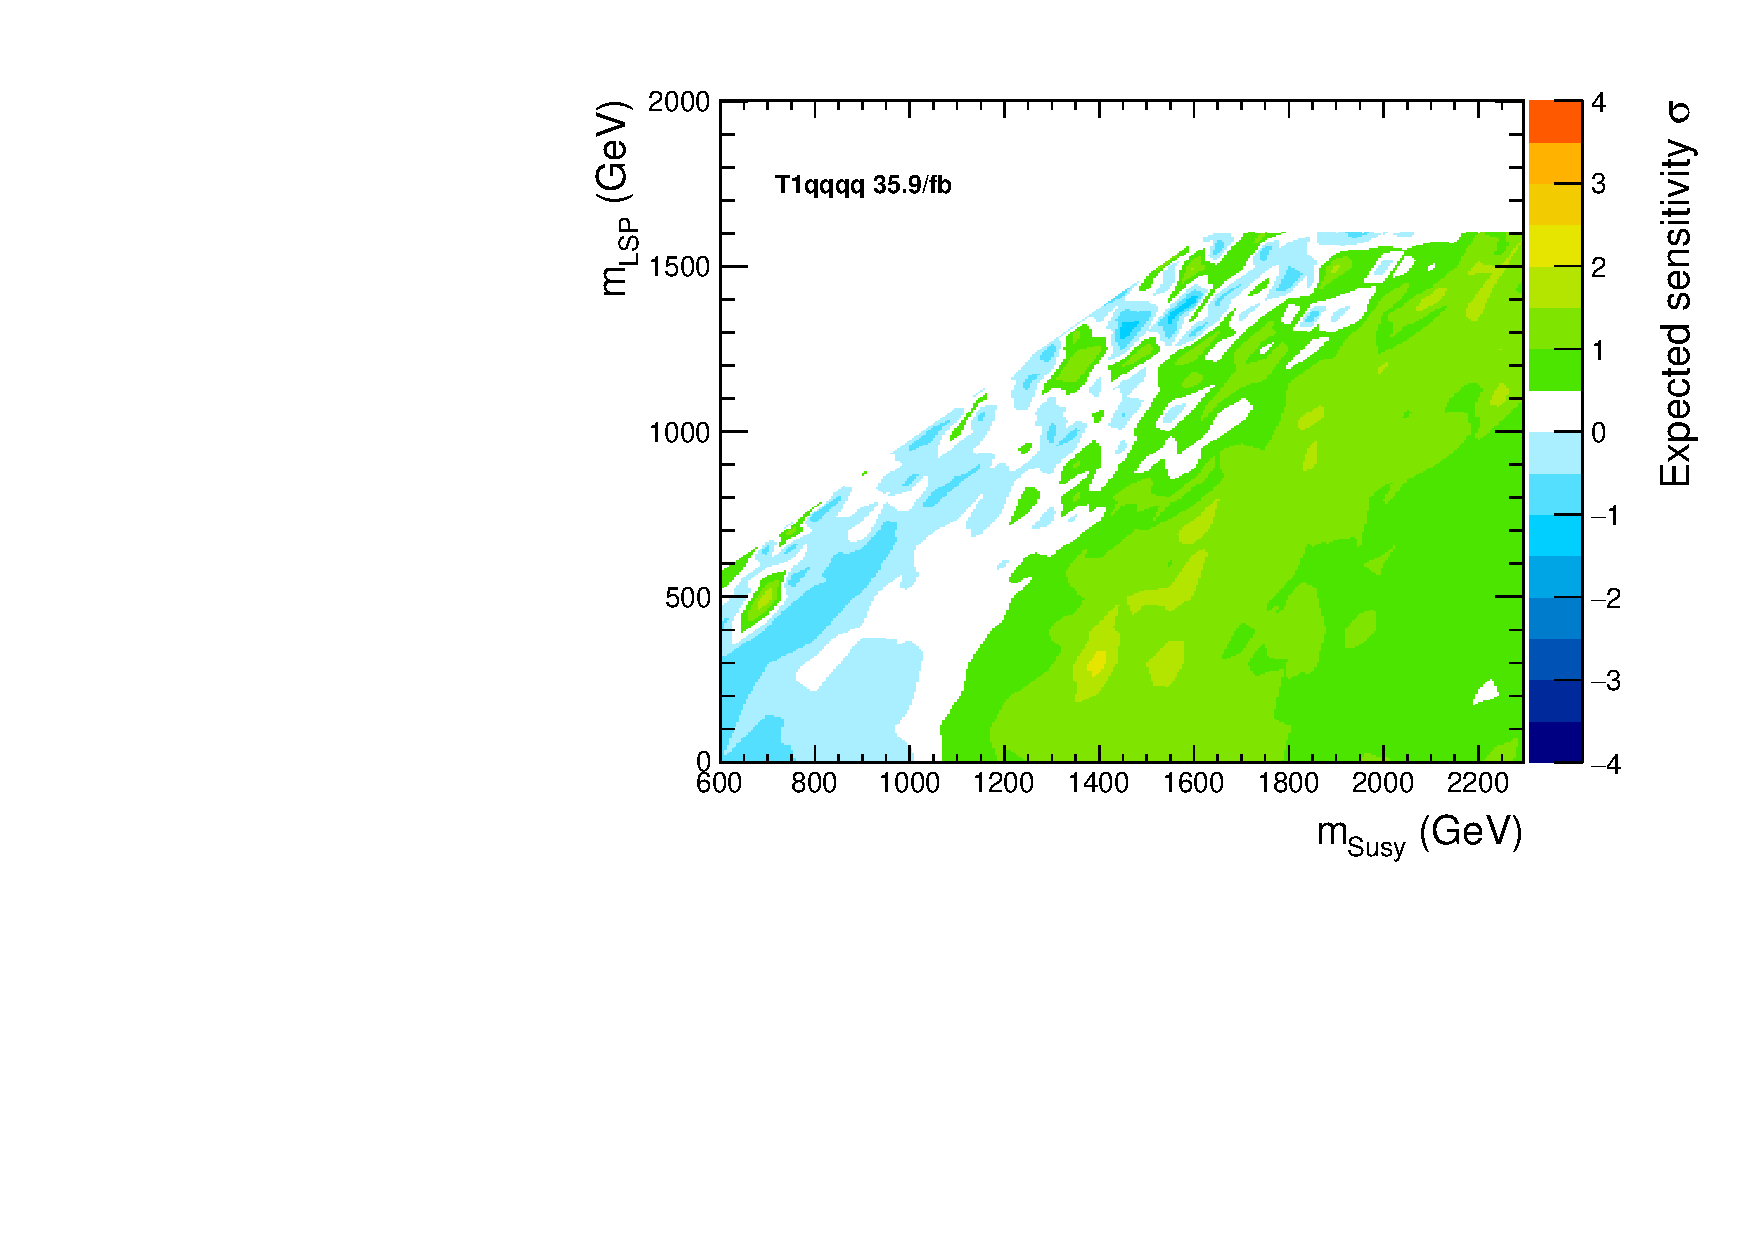
\includegraphics[width=0.45\linewidth]{figures/LLPResults/T1qqqqLL_ctau-1_signif}
        %    \label{fig:T1qqqqLL_signif}
        %} ~~
        \caption{Top: the 95\% C.L. observed upper limit on the cross section
            (histogram), with the expected (solid black line) observed
            (solid red line) exclusion contours. Left: signal acceptance
            including all jet categories. Right: graph showing the four
            most sensitive jet categories for each mass point.
            %Bottom: local observed significance scan.
        }
        \label{fig:T1qqqqLL:ctau-0p001}
    \end{center}
\end{figure}

\newpage
\begin{figure}[h!]
    \begin{center}
        \subfigure[T1qqqqLL (\ctau = 0.01~mm): Upper limit on the cross section in the mass plane]{
            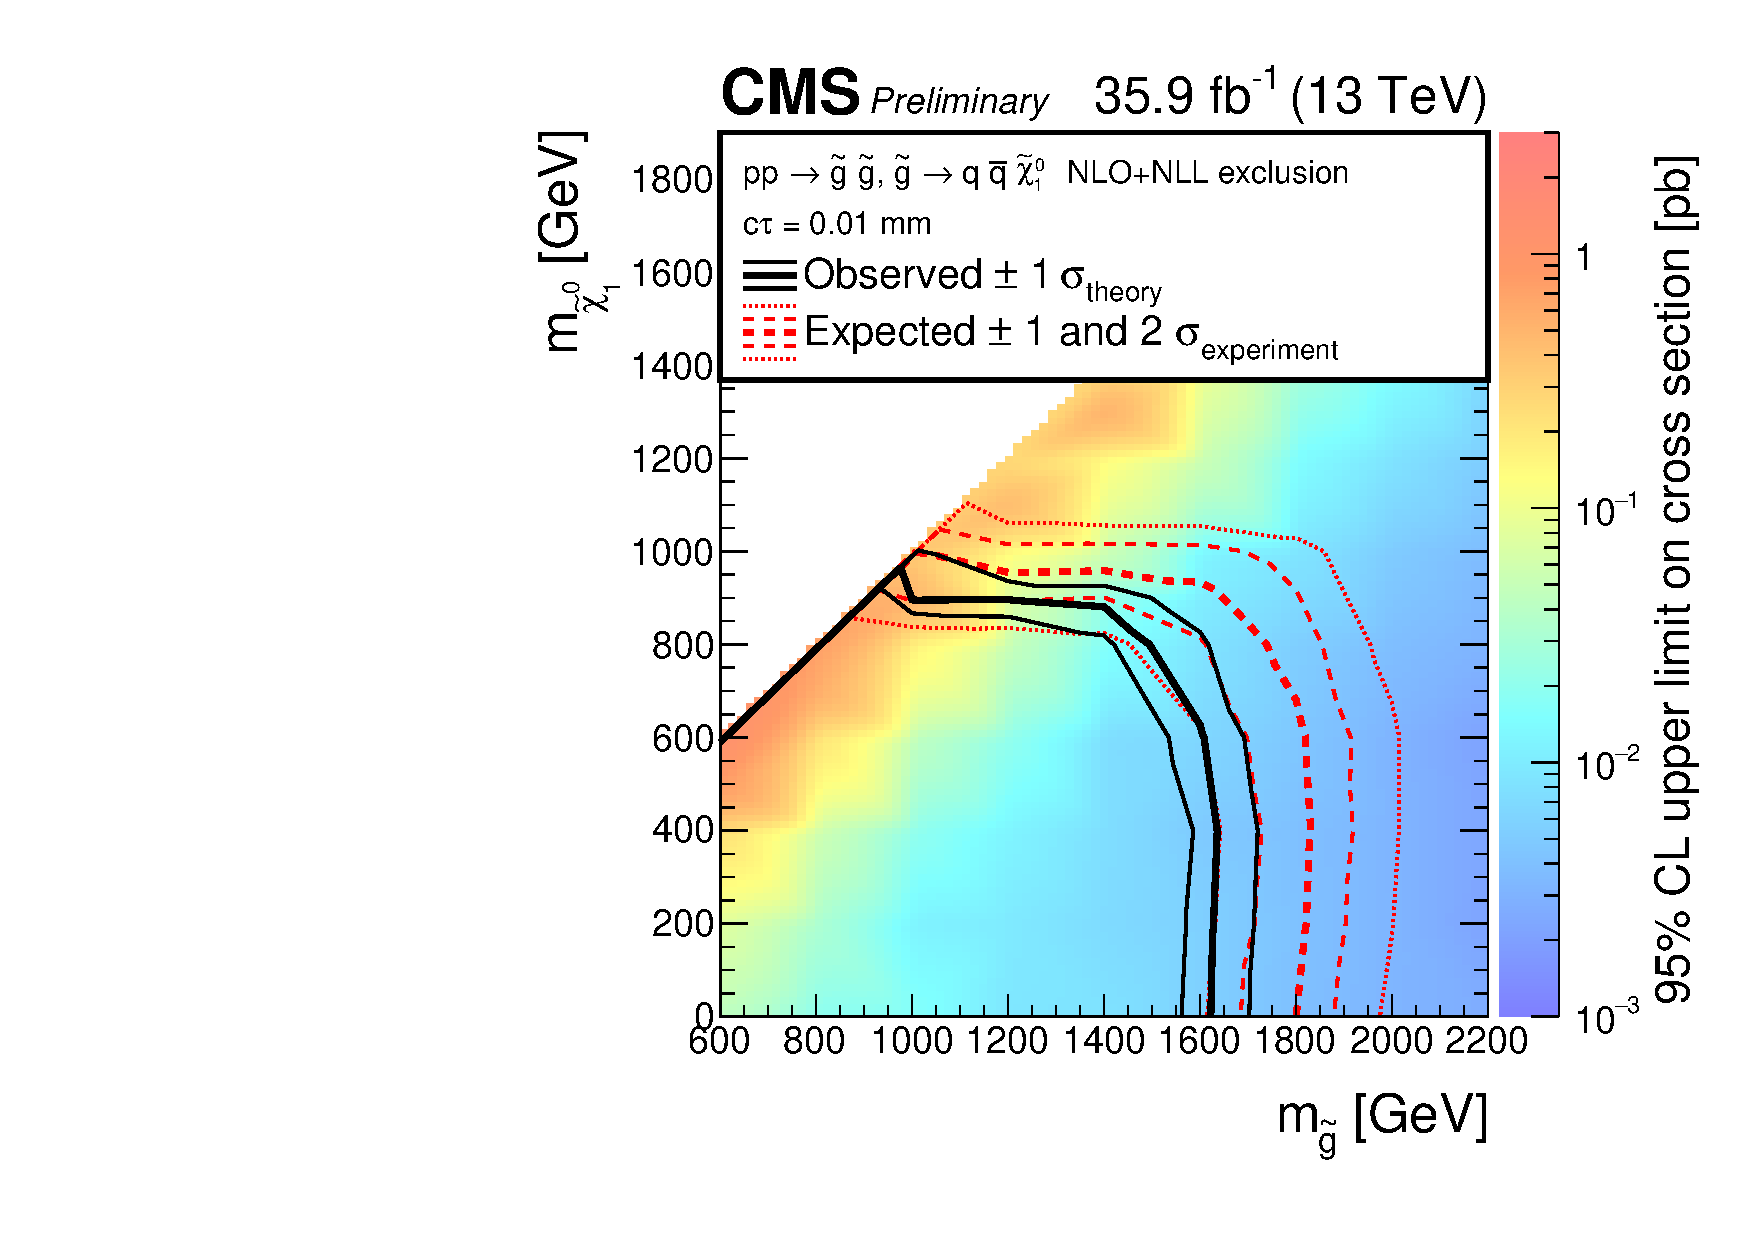
\includegraphics[width=0.6\textwidth]{figures/LLPResults/T1qqqqLL_ctau-0p01_XSEC}
            \label{fig:T1qqqqLL_excl}
        } \\
        \subfigure[T1qqqqLL (\ctau = 0.01~mm): $\epsilon_{sig}$]{
            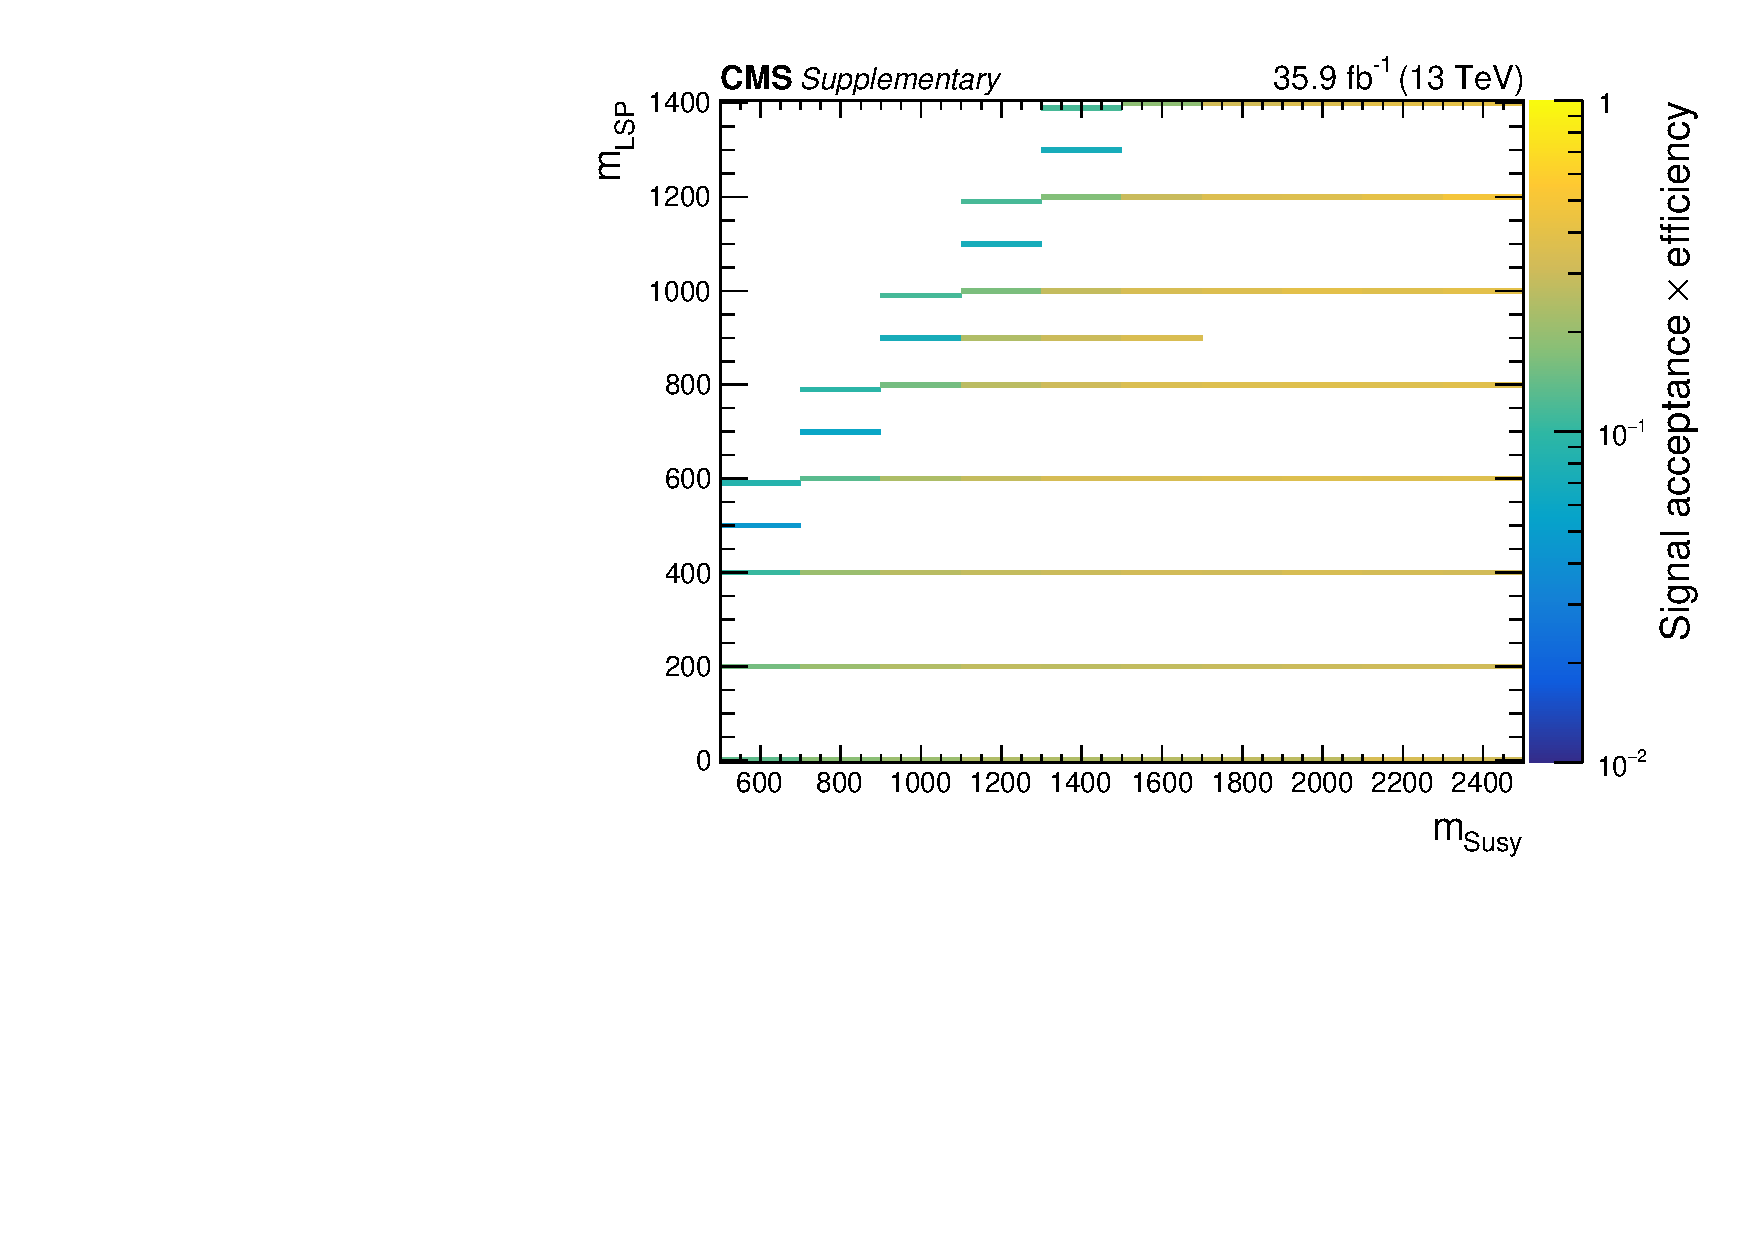
\includegraphics[width=0.45\textwidth]{figures/LLPResults/T1qqqqLL_ctau-0p01_effs}
            \label{fig:T1qqqqLL_eff}
        } ~~
        \subfigure[T1qqqqLL (\ctau = 0.01~mm): Most sensitive categories]{
            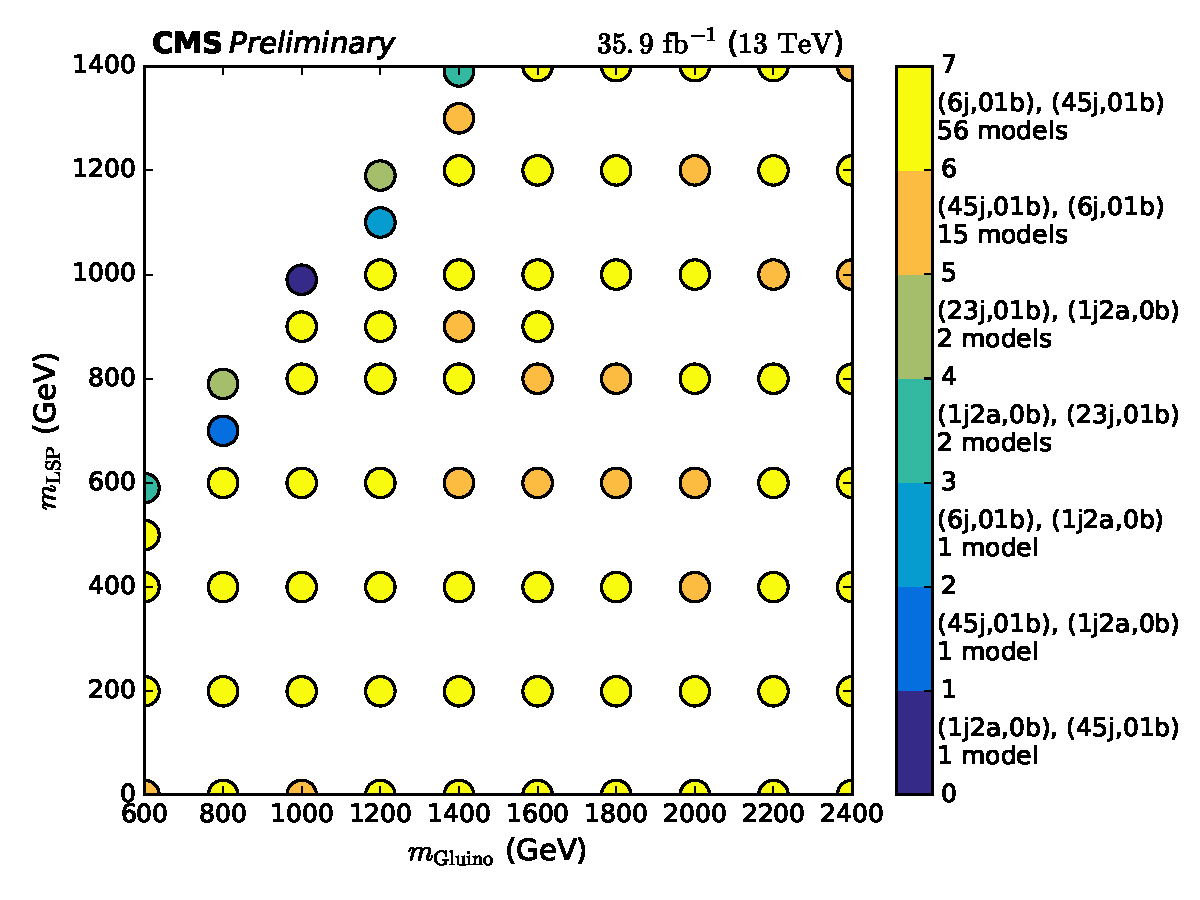
\includegraphics[width=0.45\textwidth]{figures/LLPResults/T1qqqqLL_ctau-0p01_bitMap}
            \label{fig:T1qqqqLL_bitMap}
        } \\
        %\subfigure[T1qqqqLL (\ctau = 1~mm): Significance scan]{
        %    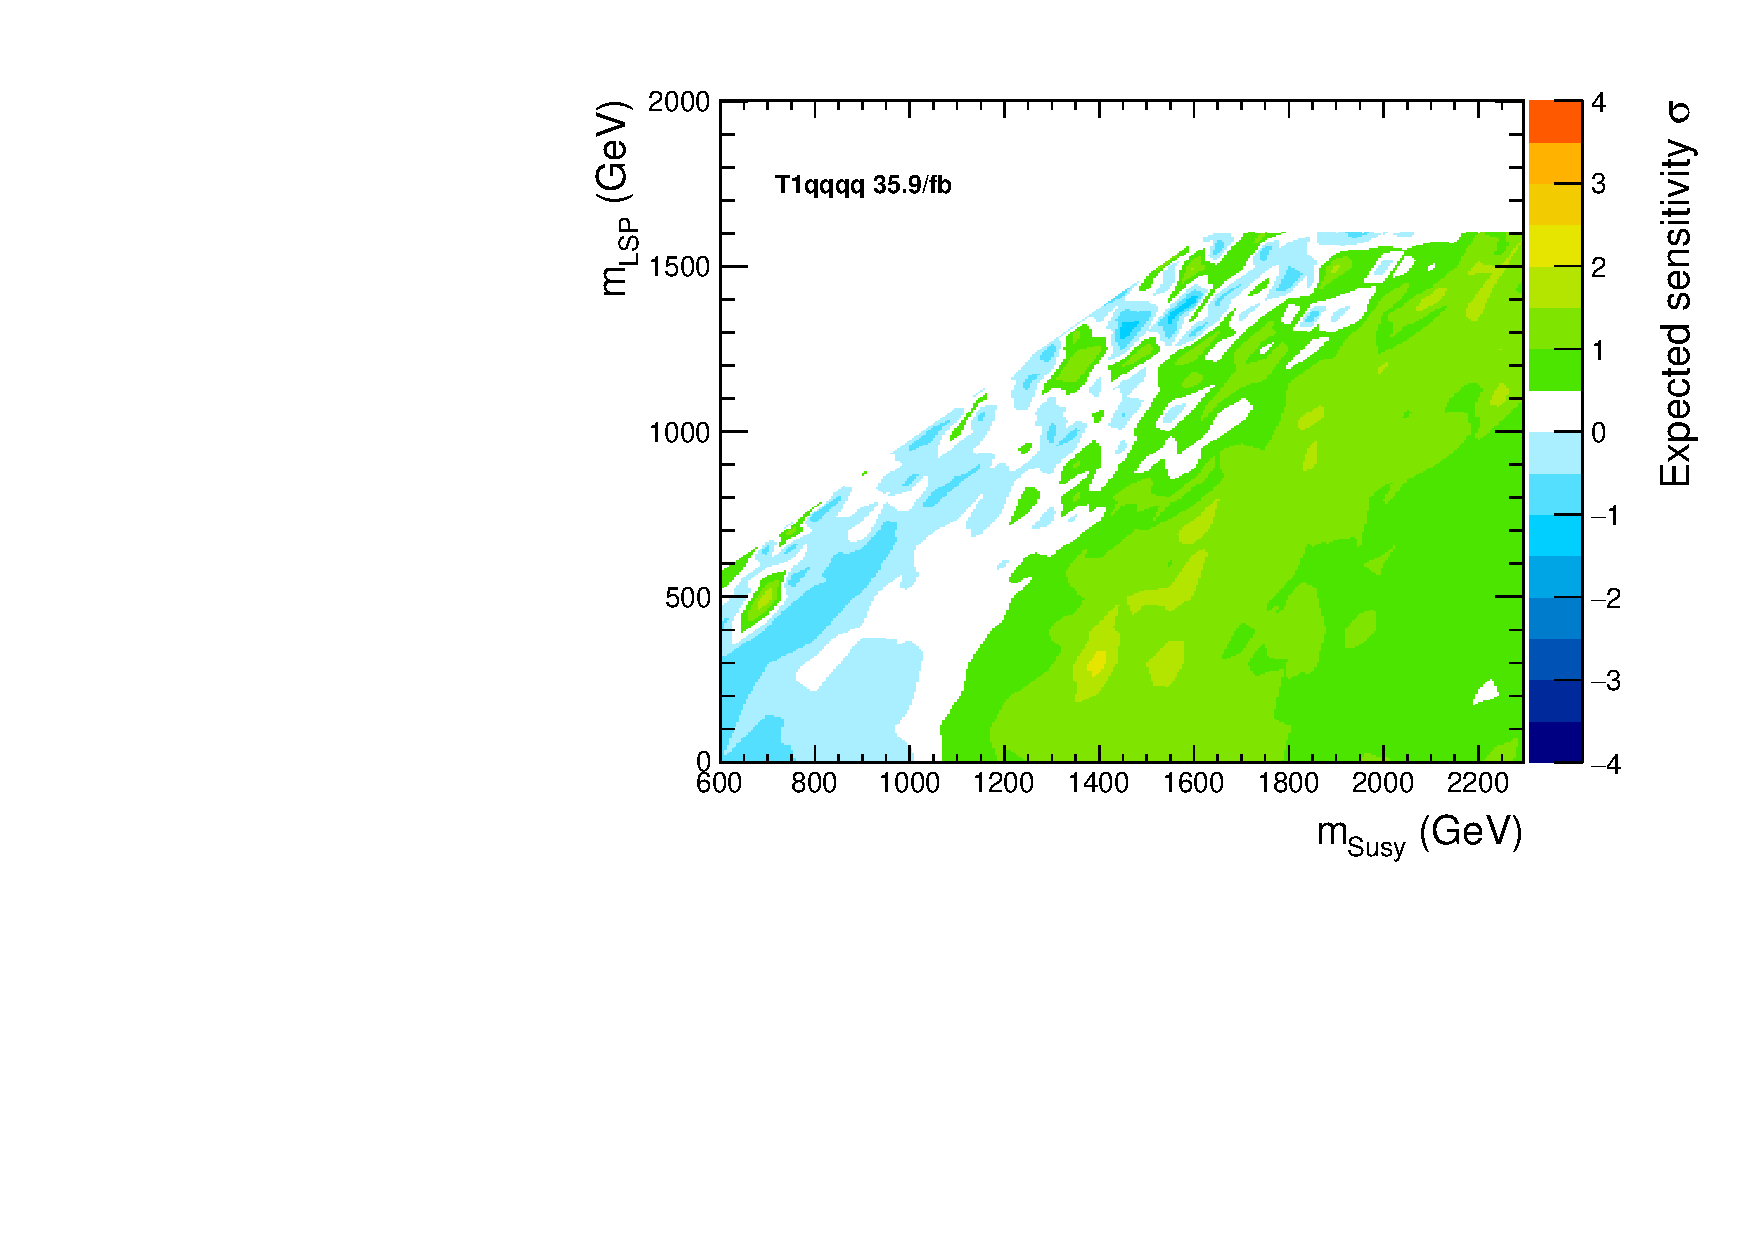
\includegraphics[width=0.45\linewidth]{figures/LLPResults/T1qqqqLL_ctau-1_signif}
        %    \label{fig:T1qqqqLL_signif}
        %} ~~
        \caption{Top: the 95\% C.L. observed upper limit on the cross section
            (histogram), with the expected (solid black line) observed
            (solid red line) exclusion contours. Left: signal acceptance
            including all jet categories. Right: graph showing the four
            most sensitive jet categories for each mass point.
            %Bottom: local observed significance scan.
        }
        \label{fig:T1qqqqLL:ctau-0p01}
    \end{center}
\end{figure}

\newpage
\begin{figure}[h!]
    \begin{center}
        \subfigure[T1qqqqLL (\ctau = 0.1~mm): Upper limit on the cross section in the mass plane]{
            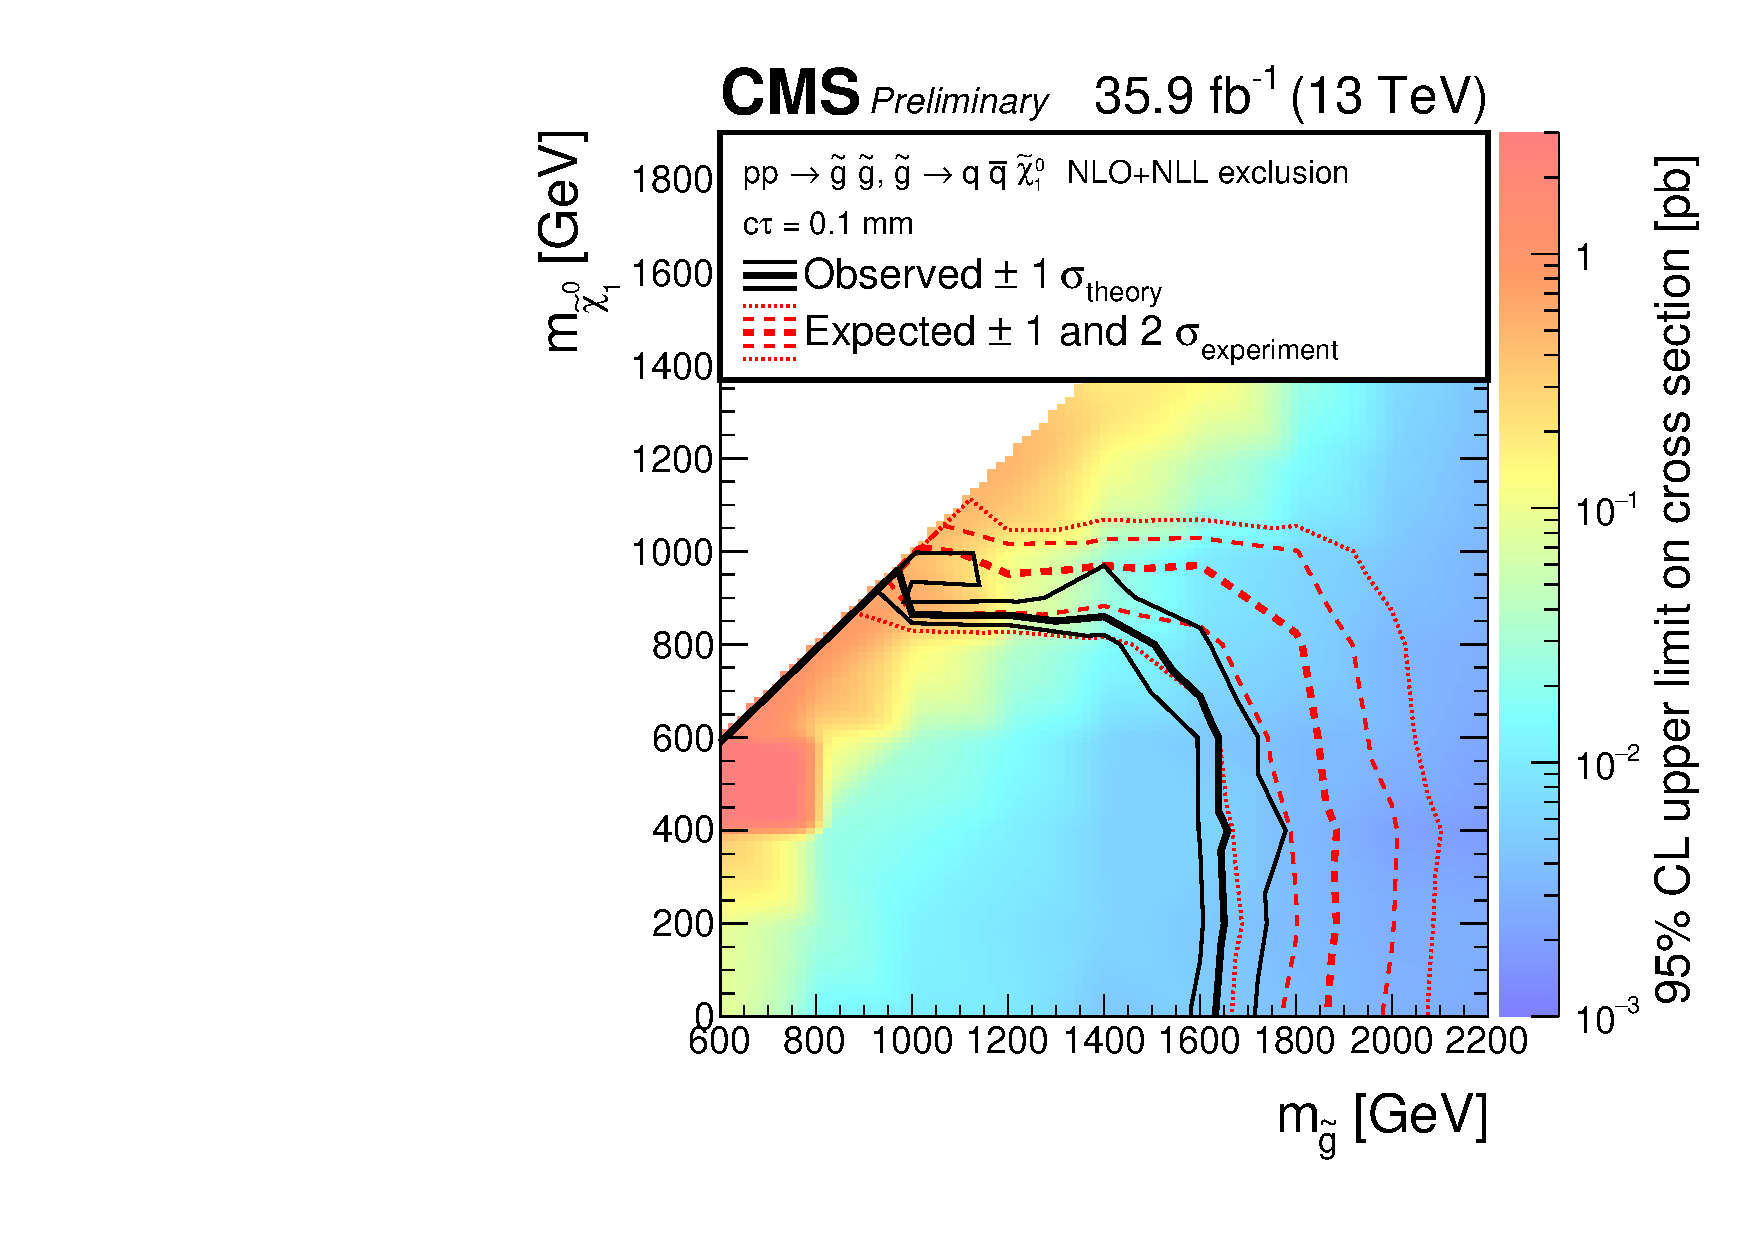
\includegraphics[width=0.6\textwidth]{figures/LLPResults/T1qqqqLL_ctau-0p1_XSEC}
            \label{fig:T1qqqqLL_excl}
        } \\
        \subfigure[T1qqqqLL (\ctau = 0.1~mm): $\epsilon_{sig}$]{
            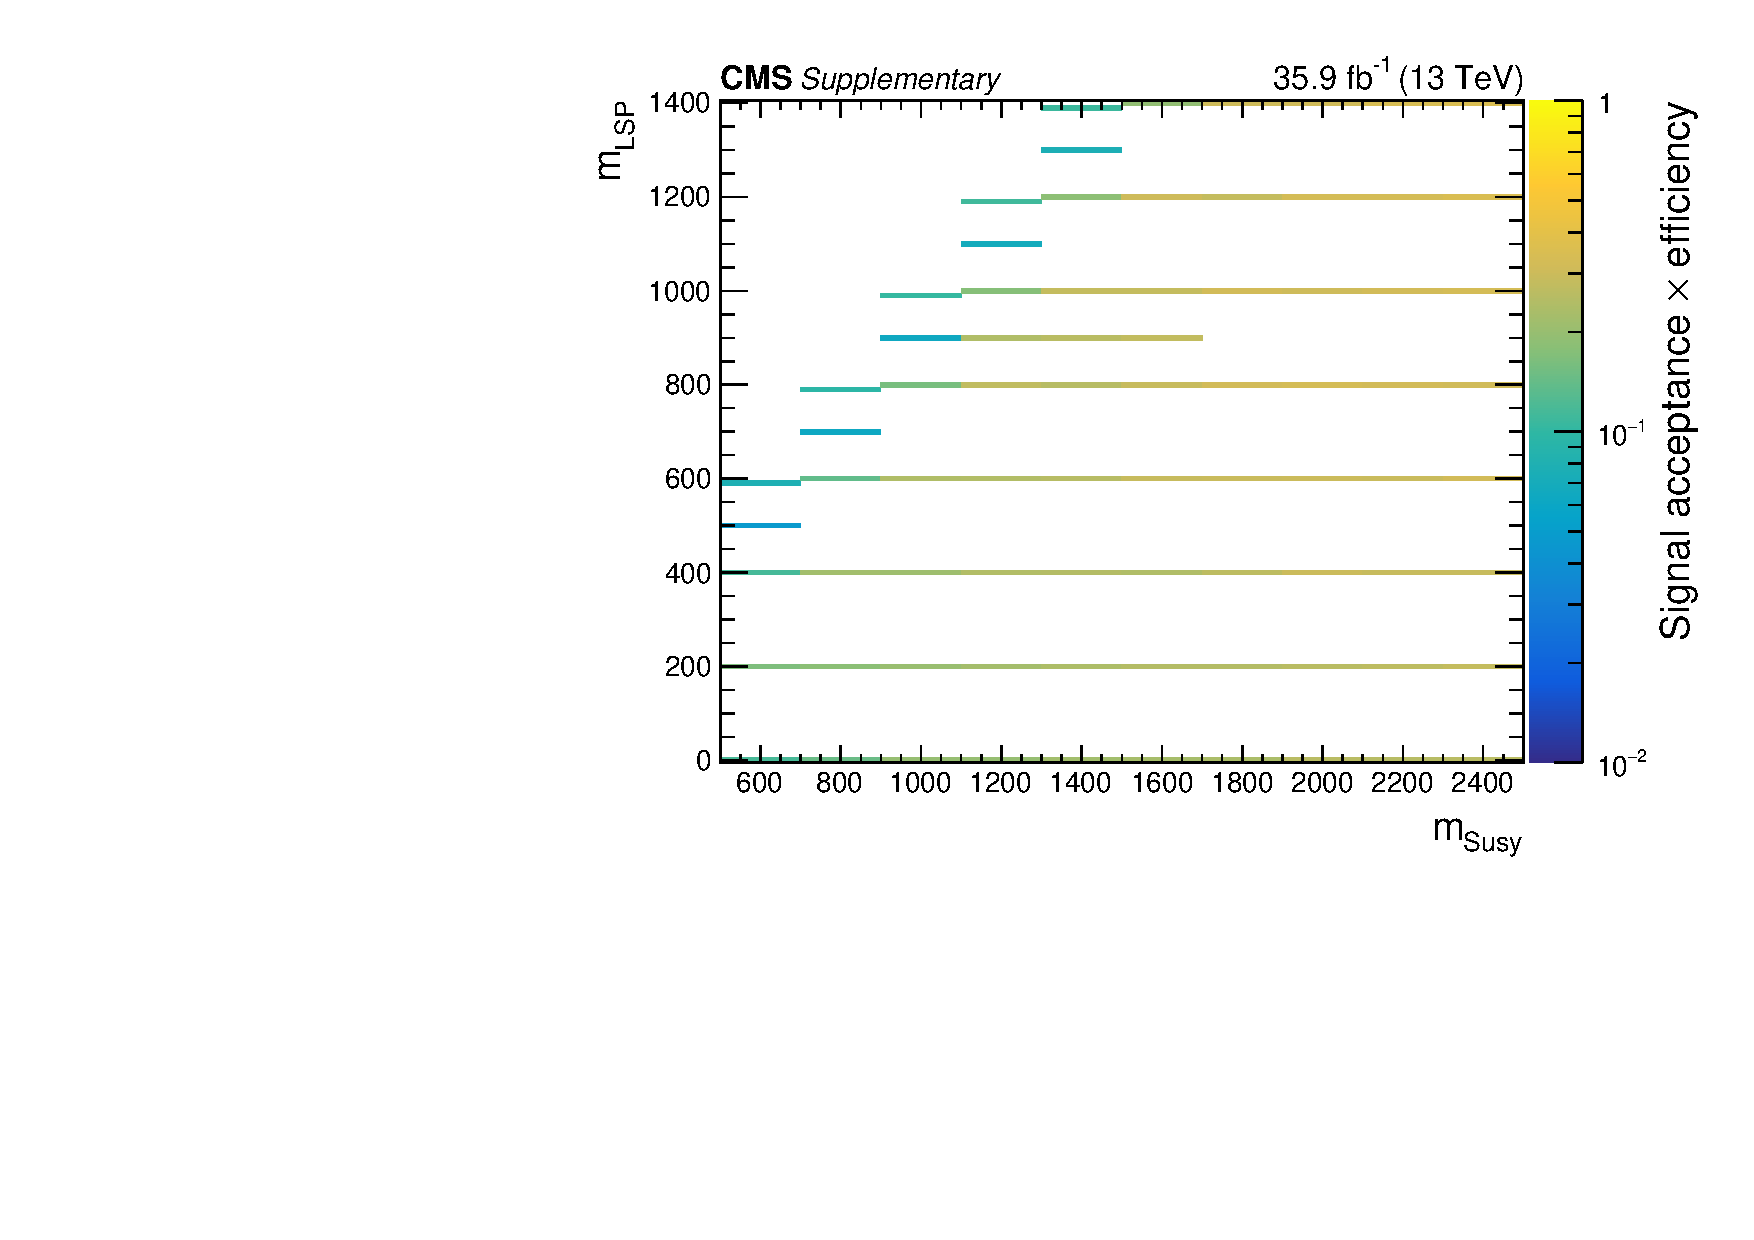
\includegraphics[width=0.45\textwidth]{figures/LLPResults/T1qqqqLL_ctau-0p1_effs}
            \label{fig:T1qqqqLL_eff}
        } ~~
        \subfigure[T1qqqqLL (\ctau = 0.1~mm): Most sensitive categories]{
            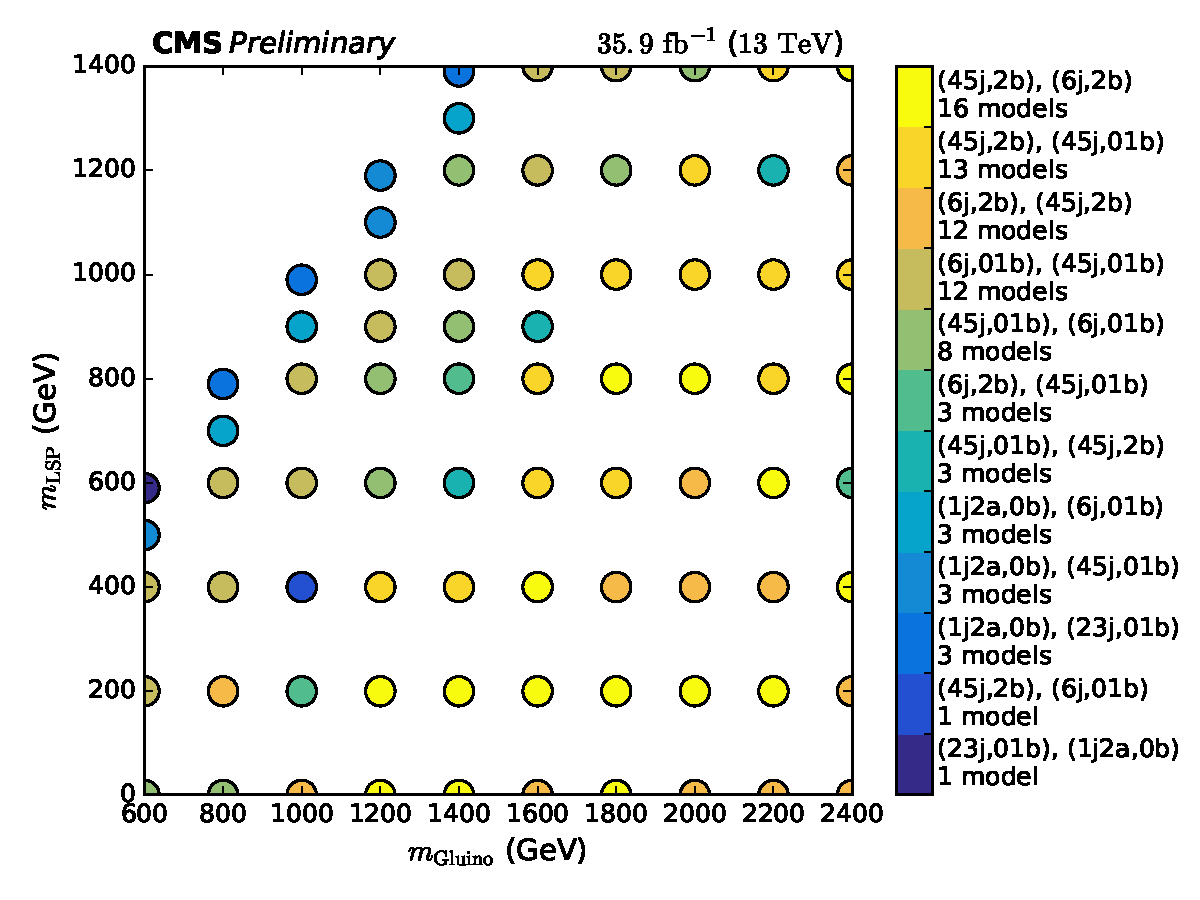
\includegraphics[width=0.45\textwidth]{figures/LLPResults/T1qqqqLL_ctau-0p1_bitMap}
            \label{fig:T1qqqqLL_bitMap}
        } \\
        %\subfigure[T1qqqqLL (\ctau = 1~mm): Significance scan]{
        %    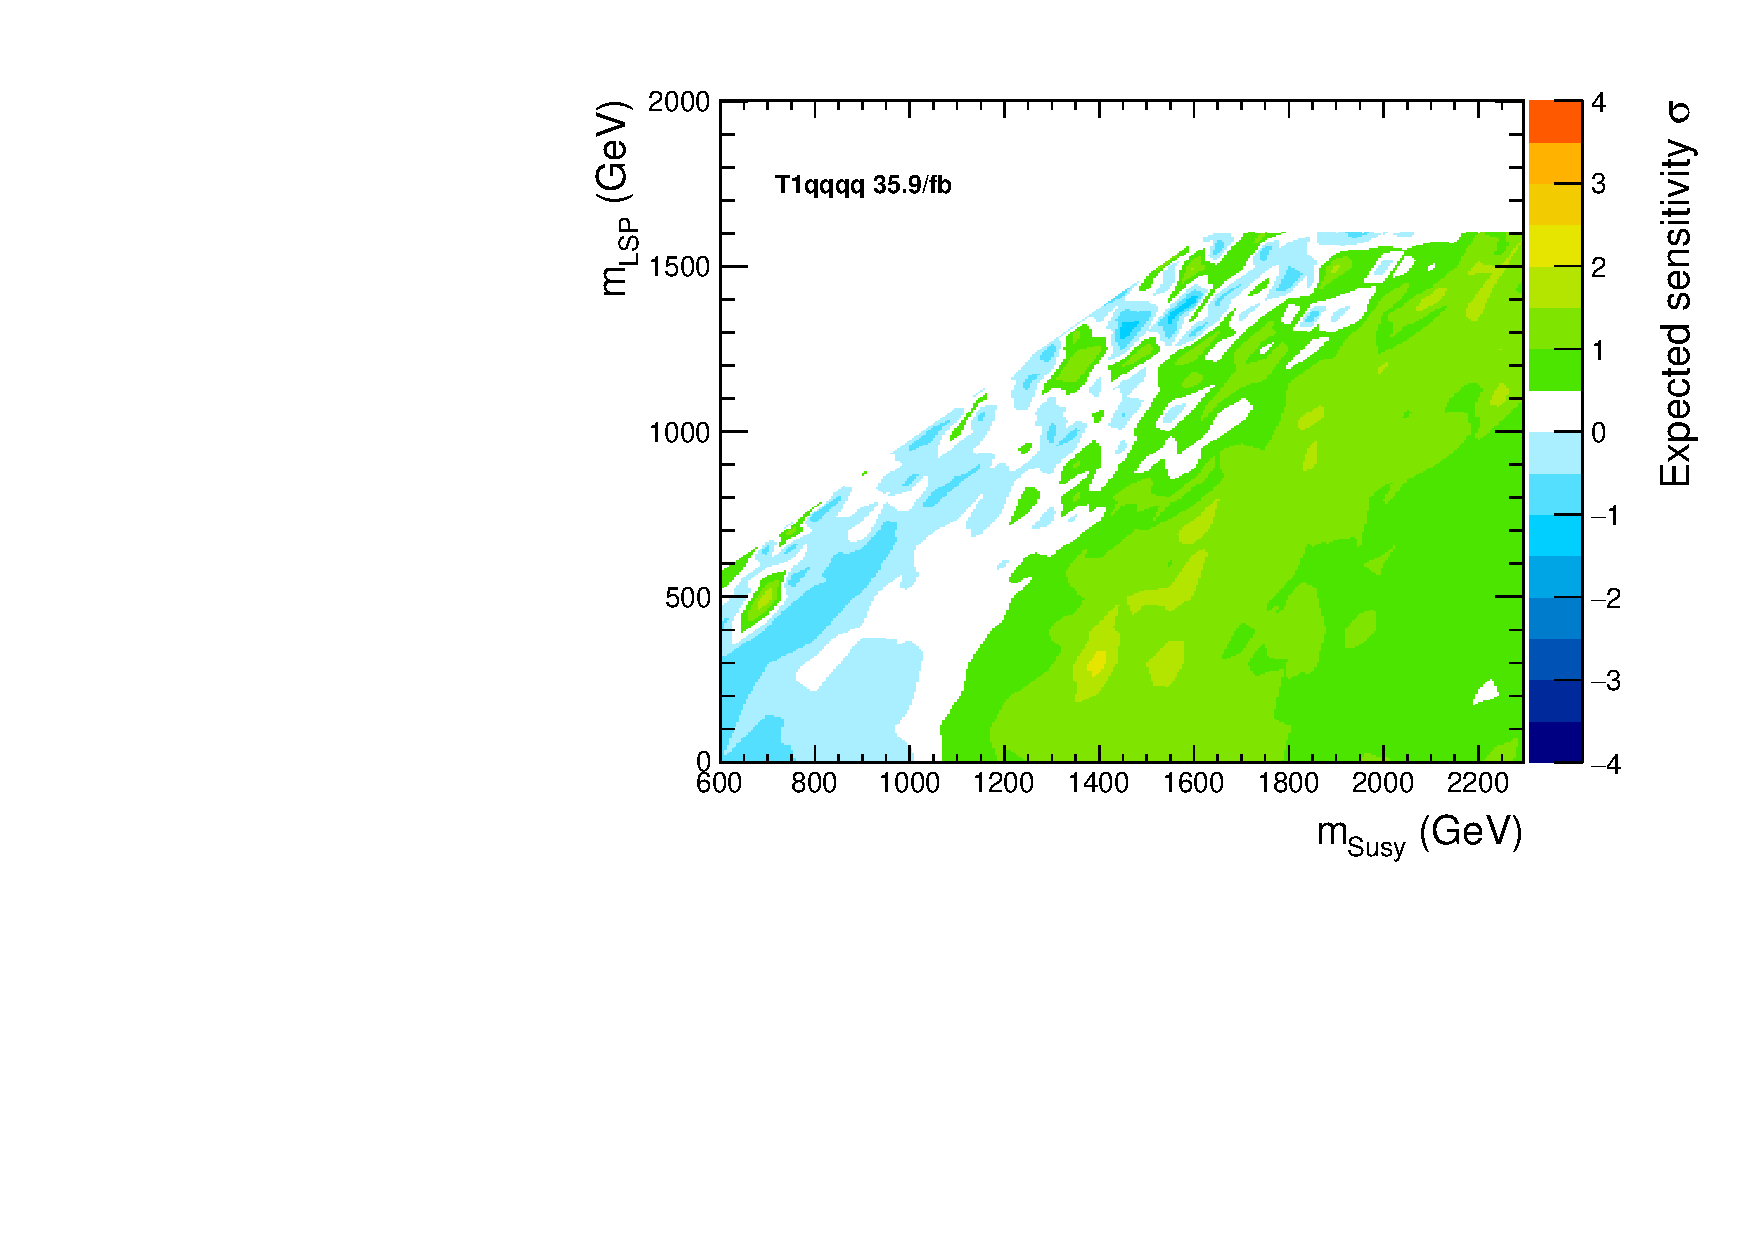
\includegraphics[width=0.45\linewidth]{figures/LLPResults/T1qqqqLL_ctau-1_signif}
        %    \label{fig:T1qqqqLL_signif}
        %} ~~
        \caption{Top: the 95\% C.L. observed upper limit on the cross section
            (histogram), with the expected (solid black line) observed
            (solid red line) exclusion contours. Left: signal acceptance
            including all jet categories. Right: graph showing the four
            most sensitive jet categories for each mass point.
            %Bottom: local observed significance scan.
        }
        \label{fig:T1qqqqLL:ctau-0p1}
    \end{center}
\end{figure}

\newpage
\begin{figure}[h!]
    \begin{center}
        \subfigure[T1qqqqLL (\ctau = 1~mm): Upper limit on the cross section in the mass plane]{
            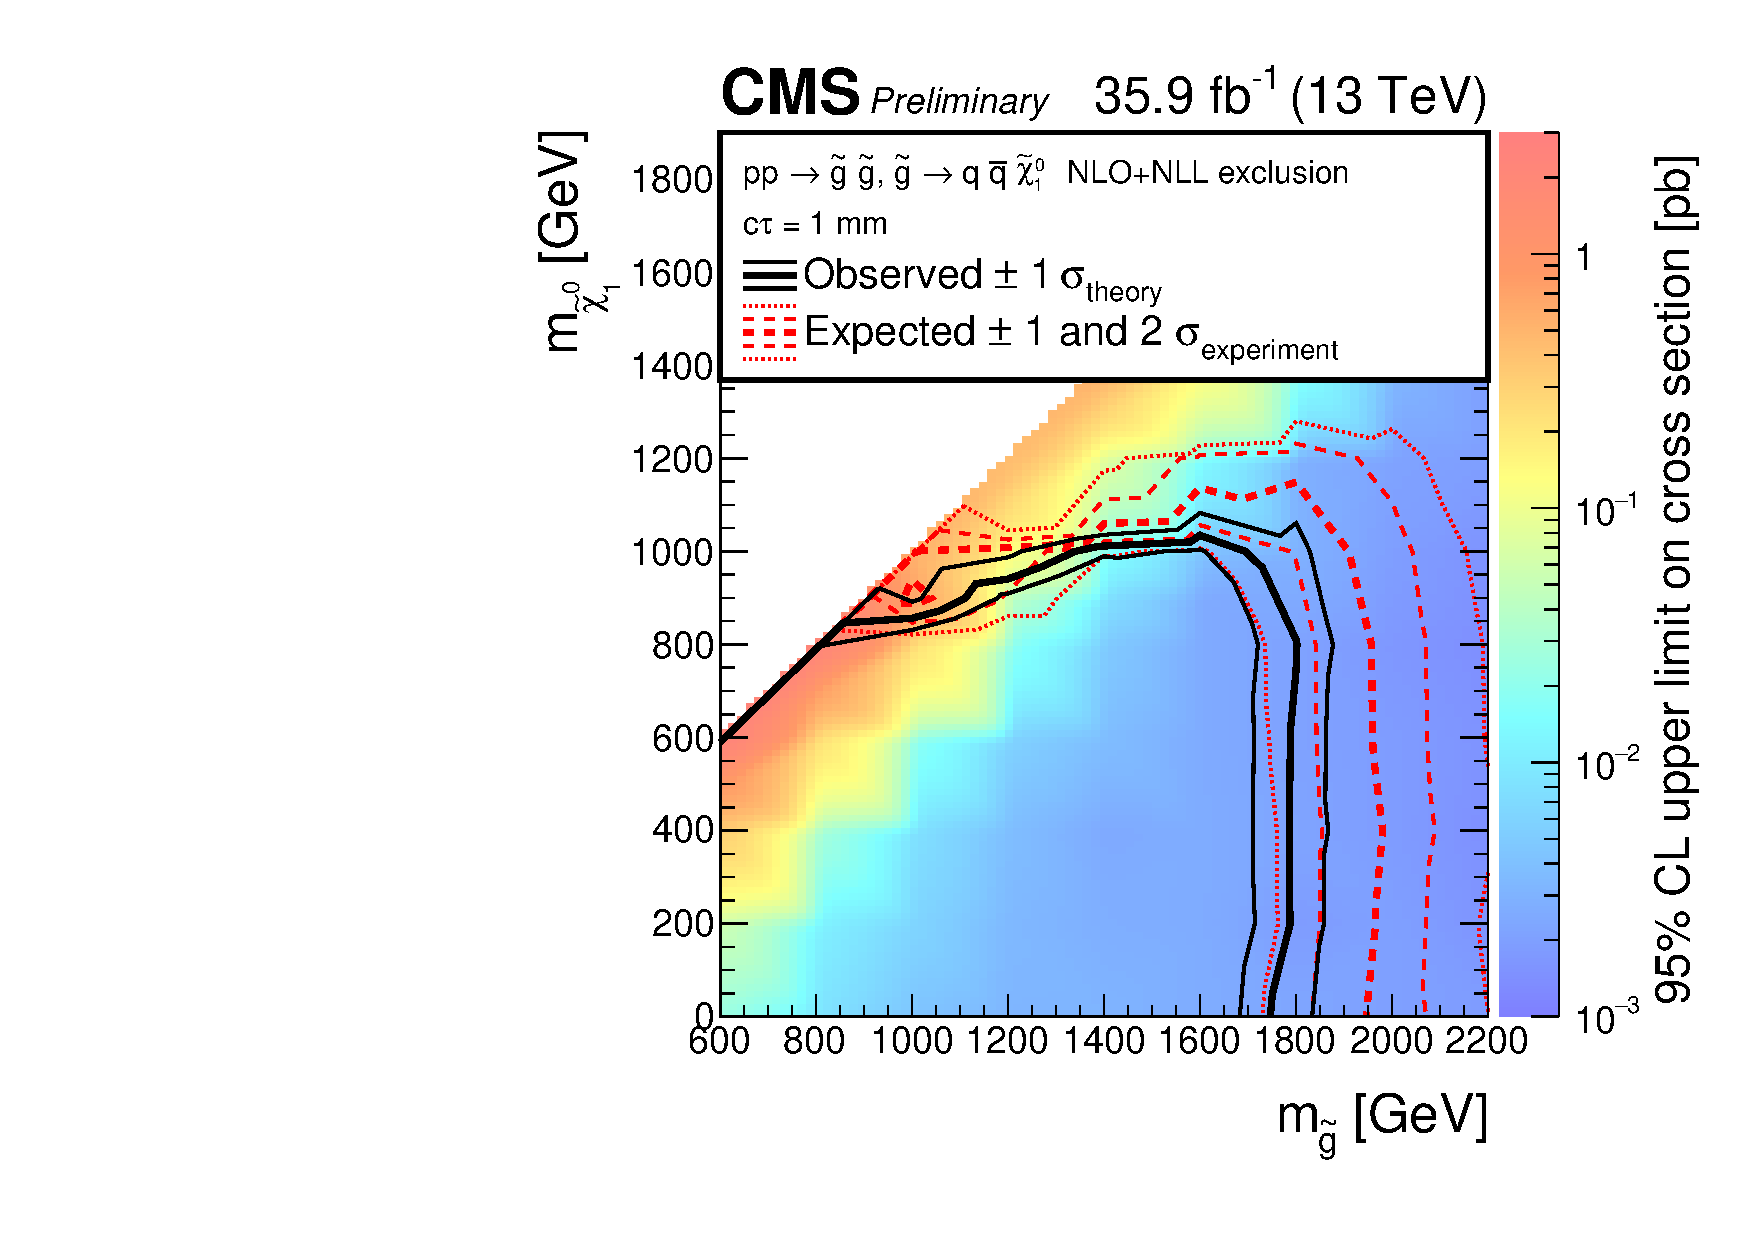
\includegraphics[width=0.6\textwidth]{figures/LLPResults/T1qqqqLL_ctau-1_XSEC}
            \label{fig:T1qqqqLL_excl}
        } \\
        \subfigure[T1qqqqLL (\ctau = 1~mm): $\epsilon_{sig}$]{
            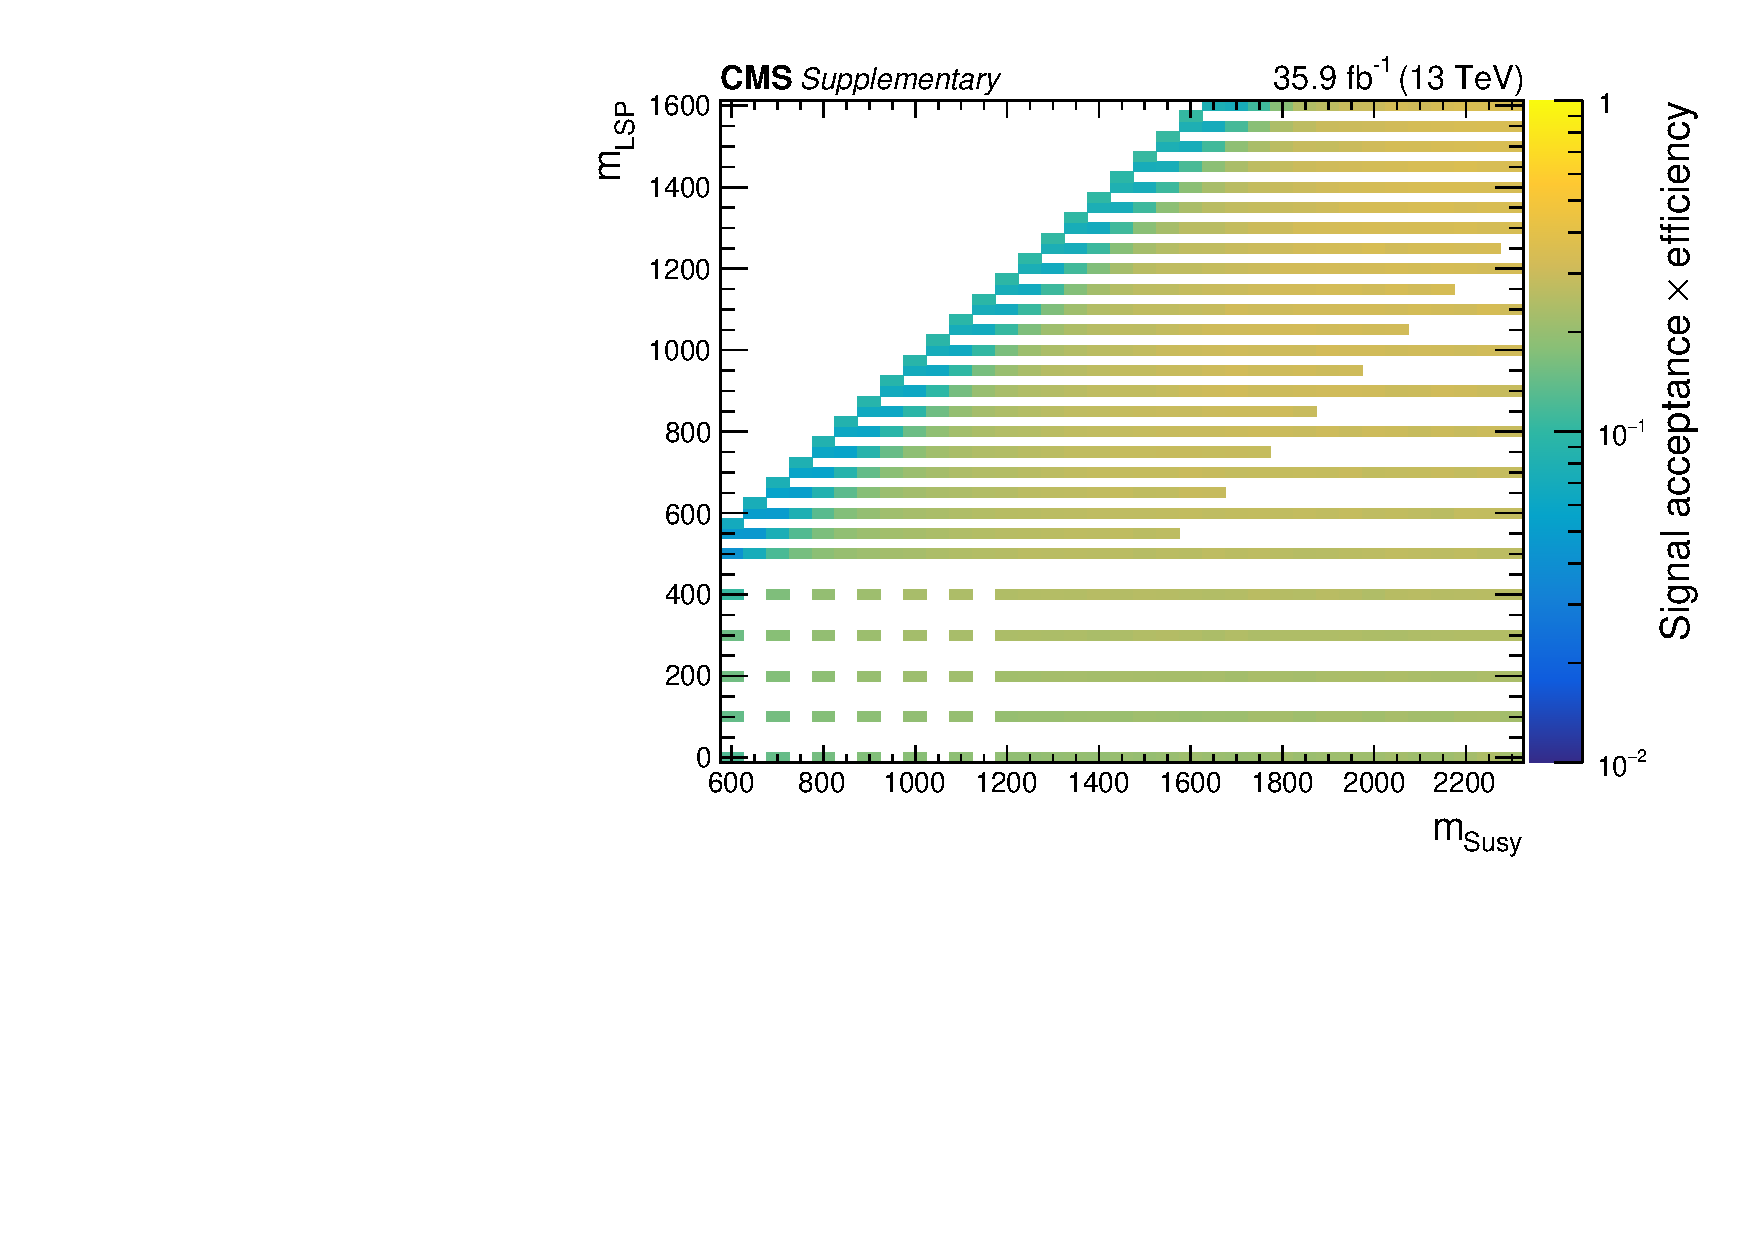
\includegraphics[width=0.45\textwidth]{figures/LLPResults/T1qqqqLL_ctau-1_effs}
            \label{fig:T1qqqqLL_eff}
        } ~~
        \subfigure[T1qqqqLL (\ctau = 1~mm): Most sensitive categories]{
            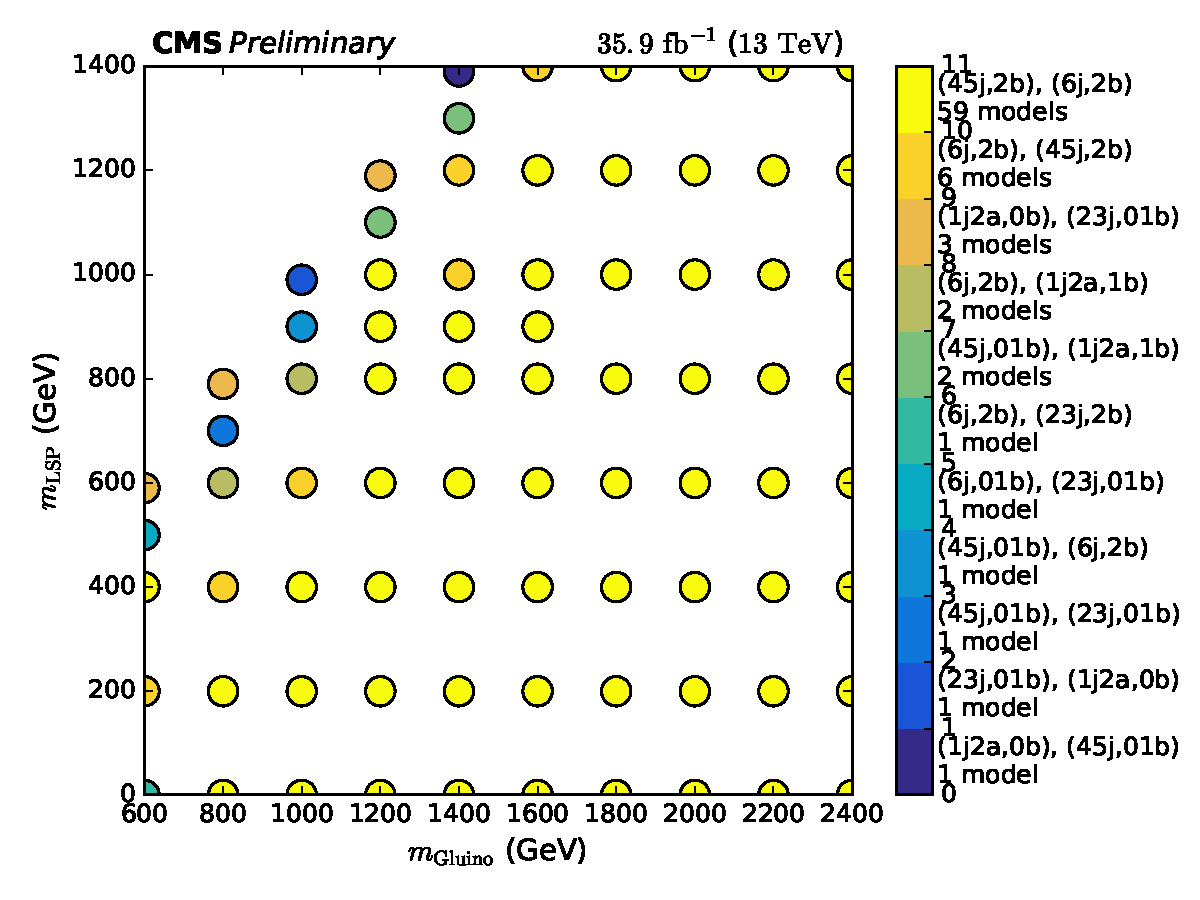
\includegraphics[width=0.45\textwidth]{figures/LLPResults/T1qqqqLL_ctau-1_bitMap}
            \label{fig:T1qqqqLL_bitMap}
        } \\
        %\subfigure[T1qqqqLL (\ctau = 1~mm): Significance scan]{
        %    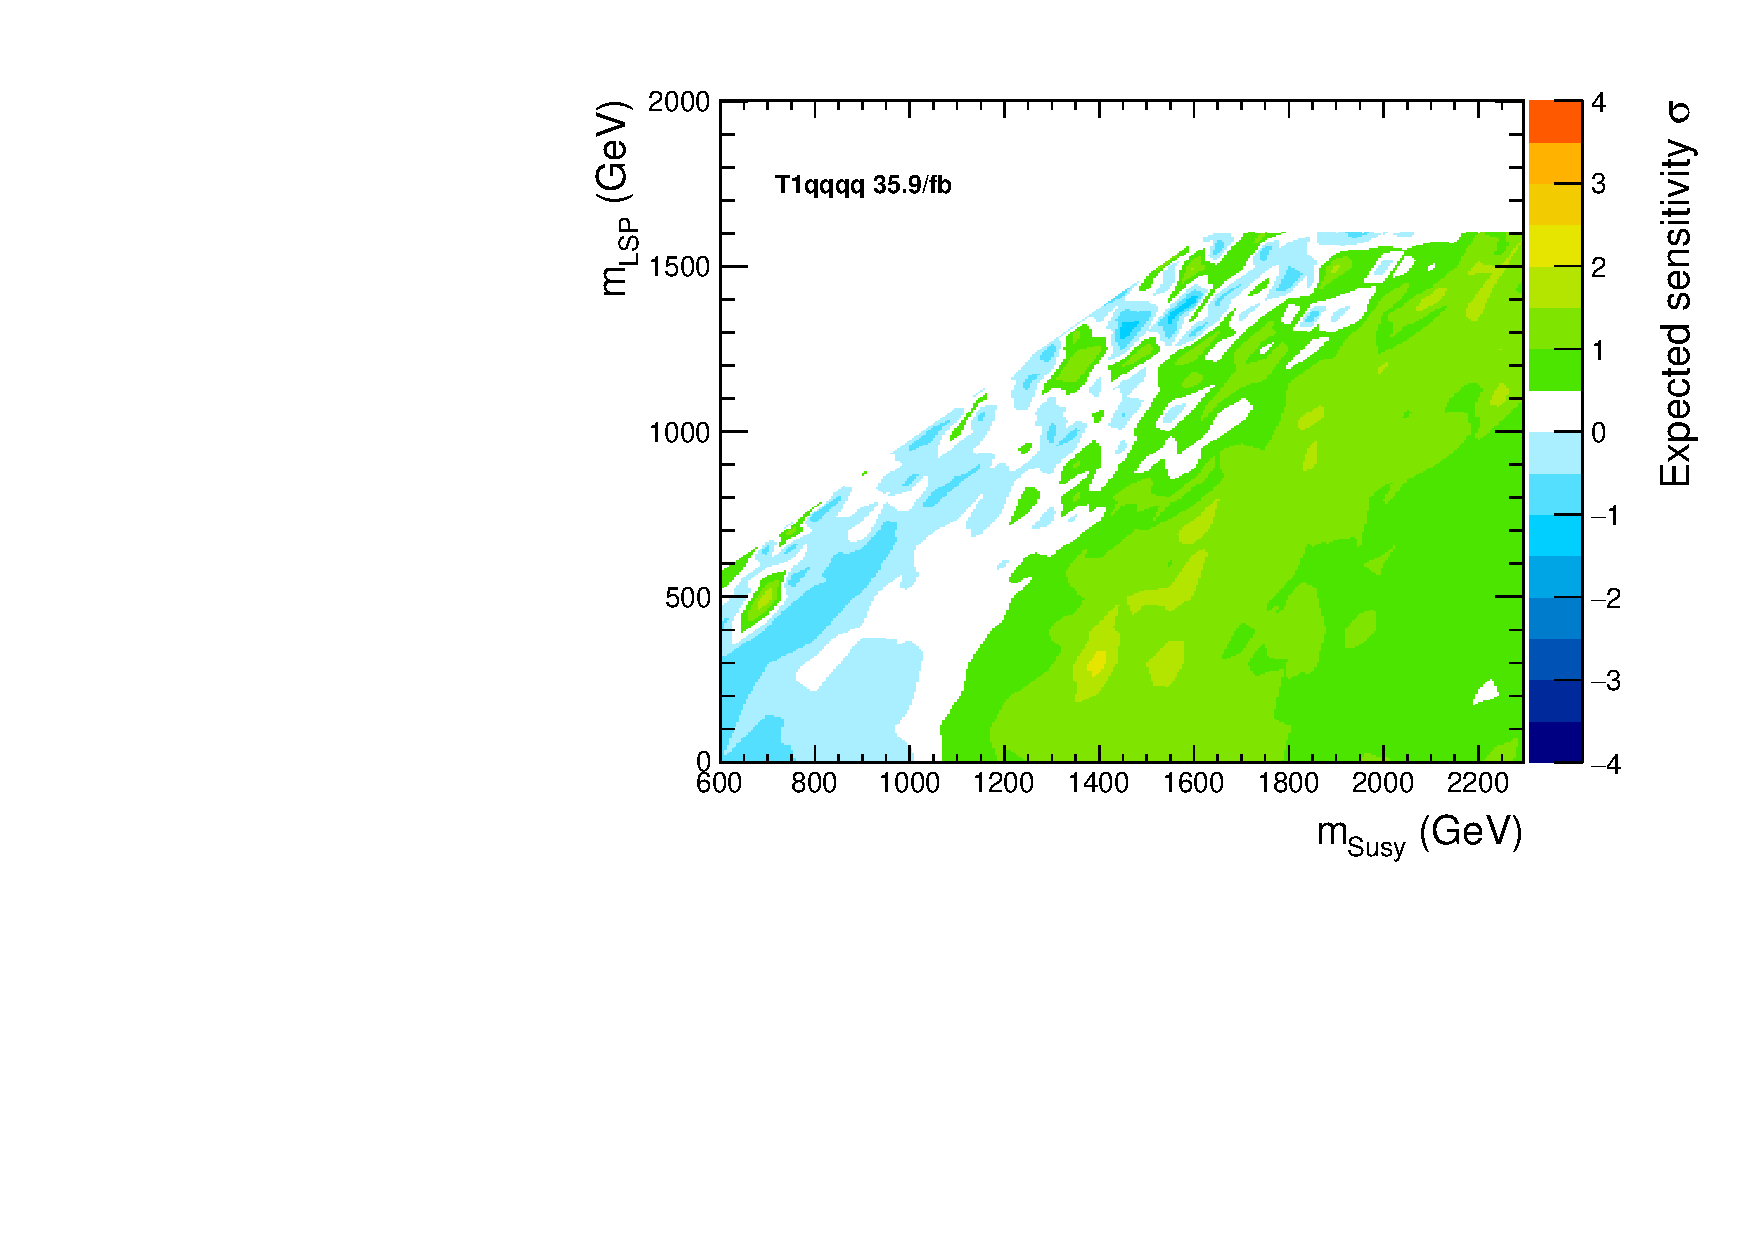
\includegraphics[width=0.45\linewidth]{figures/LLPResults/T1qqqqLL_ctau-1_signif}
        %    \label{fig:T1qqqqLL_signif}
        %} ~~
        \caption{Top: the 95\% C.L. observed upper limit on the cross section
            (histogram), with the expected (solid black line) observed
            (solid red line) exclusion contours. Left: signal acceptance
            including all jet categories. Right: graph showing the four
            most sensitive jet categories for each mass point.
            %Bottom: local observed significance scan.
        }
        \label{fig:T1qqqqLL:ctau-1}
    \end{center}
\end{figure}

\newpage
\begin{figure}[h!]
    \begin{center}
        \subfigure[T1qqqqLL (\ctau = 10~mm): Upper limit on the cross section in the mass plane]{
            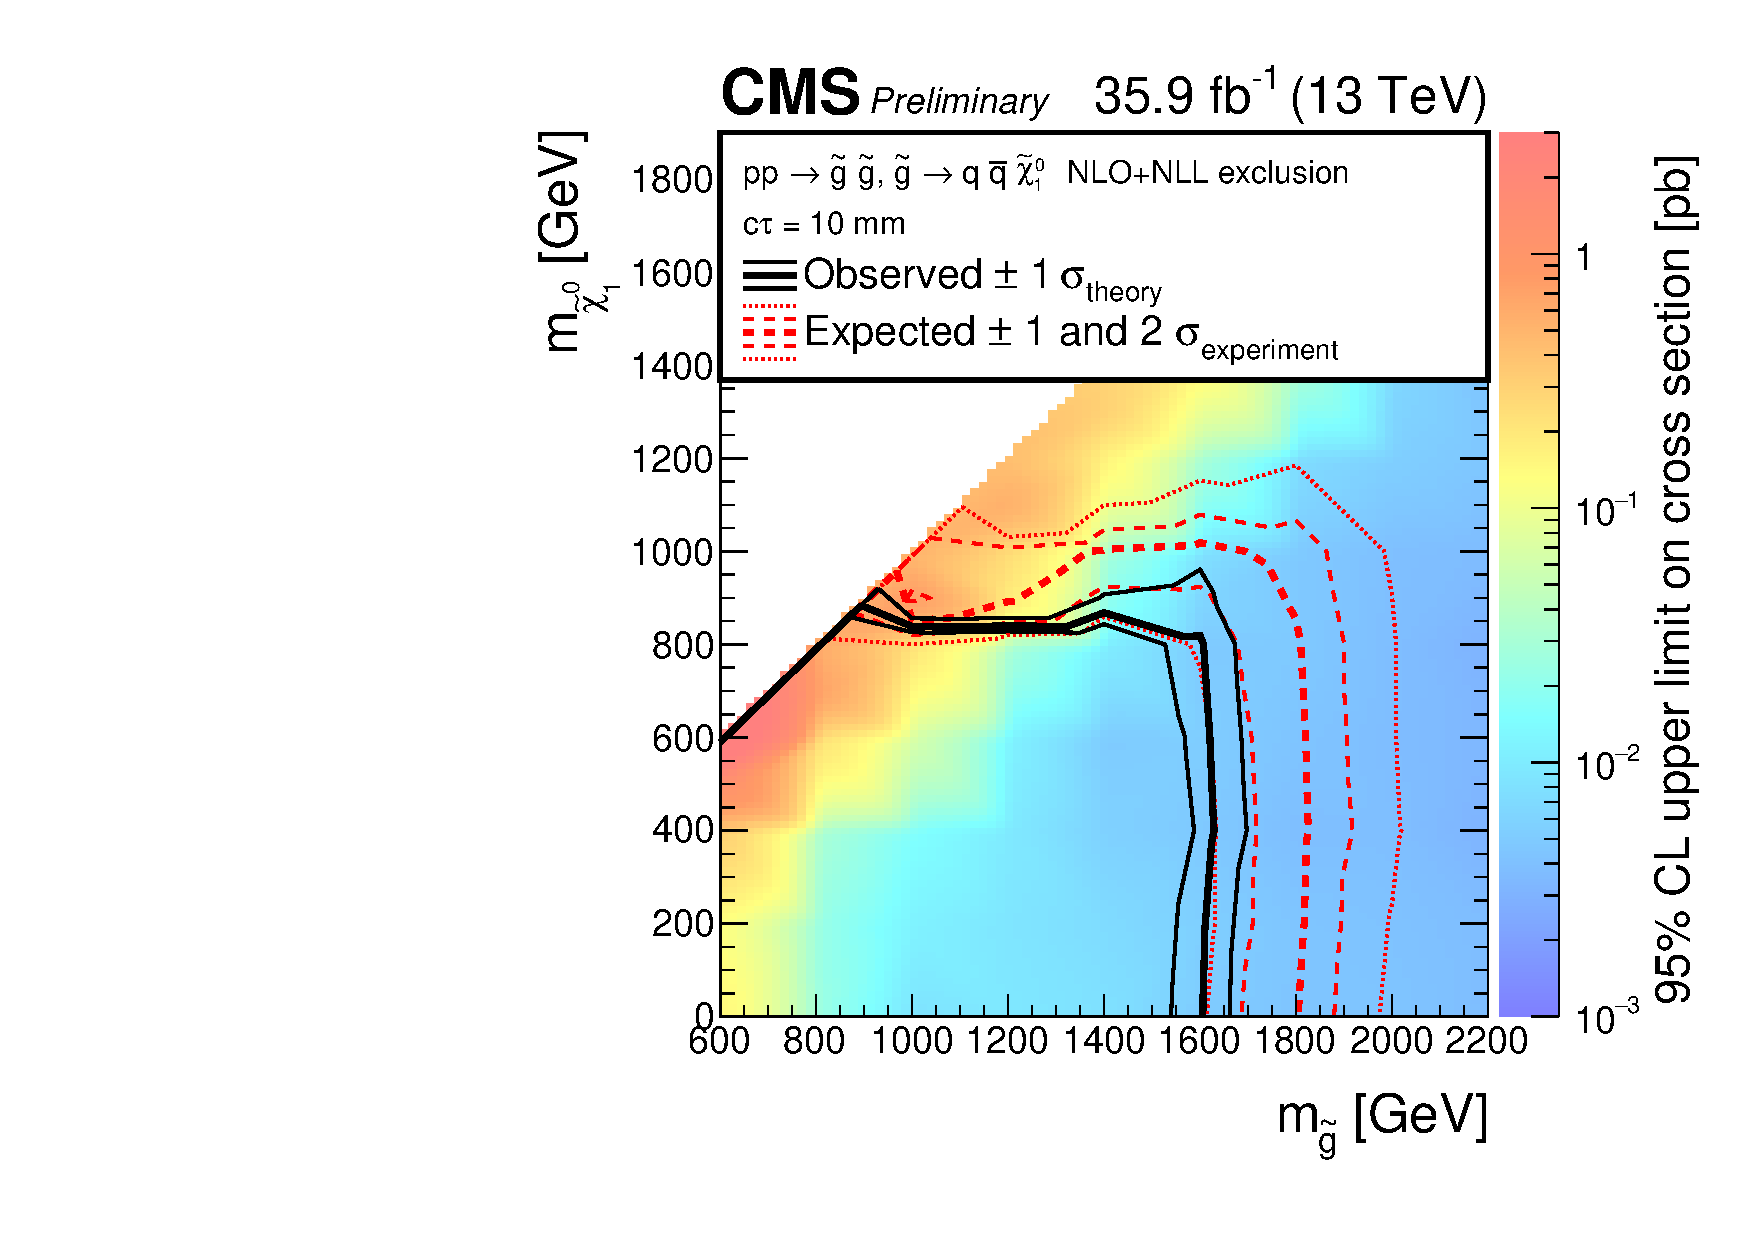
\includegraphics[width=0.6\textwidth]{figures/LLPResults/T1qqqqLL_ctau-10_XSEC}
            \label{fig:T1qqqqLL_excl}
        } \\
        \subfigure[T1qqqqLL (\ctau = 10~mm): $\epsilon_{sig}$]{
            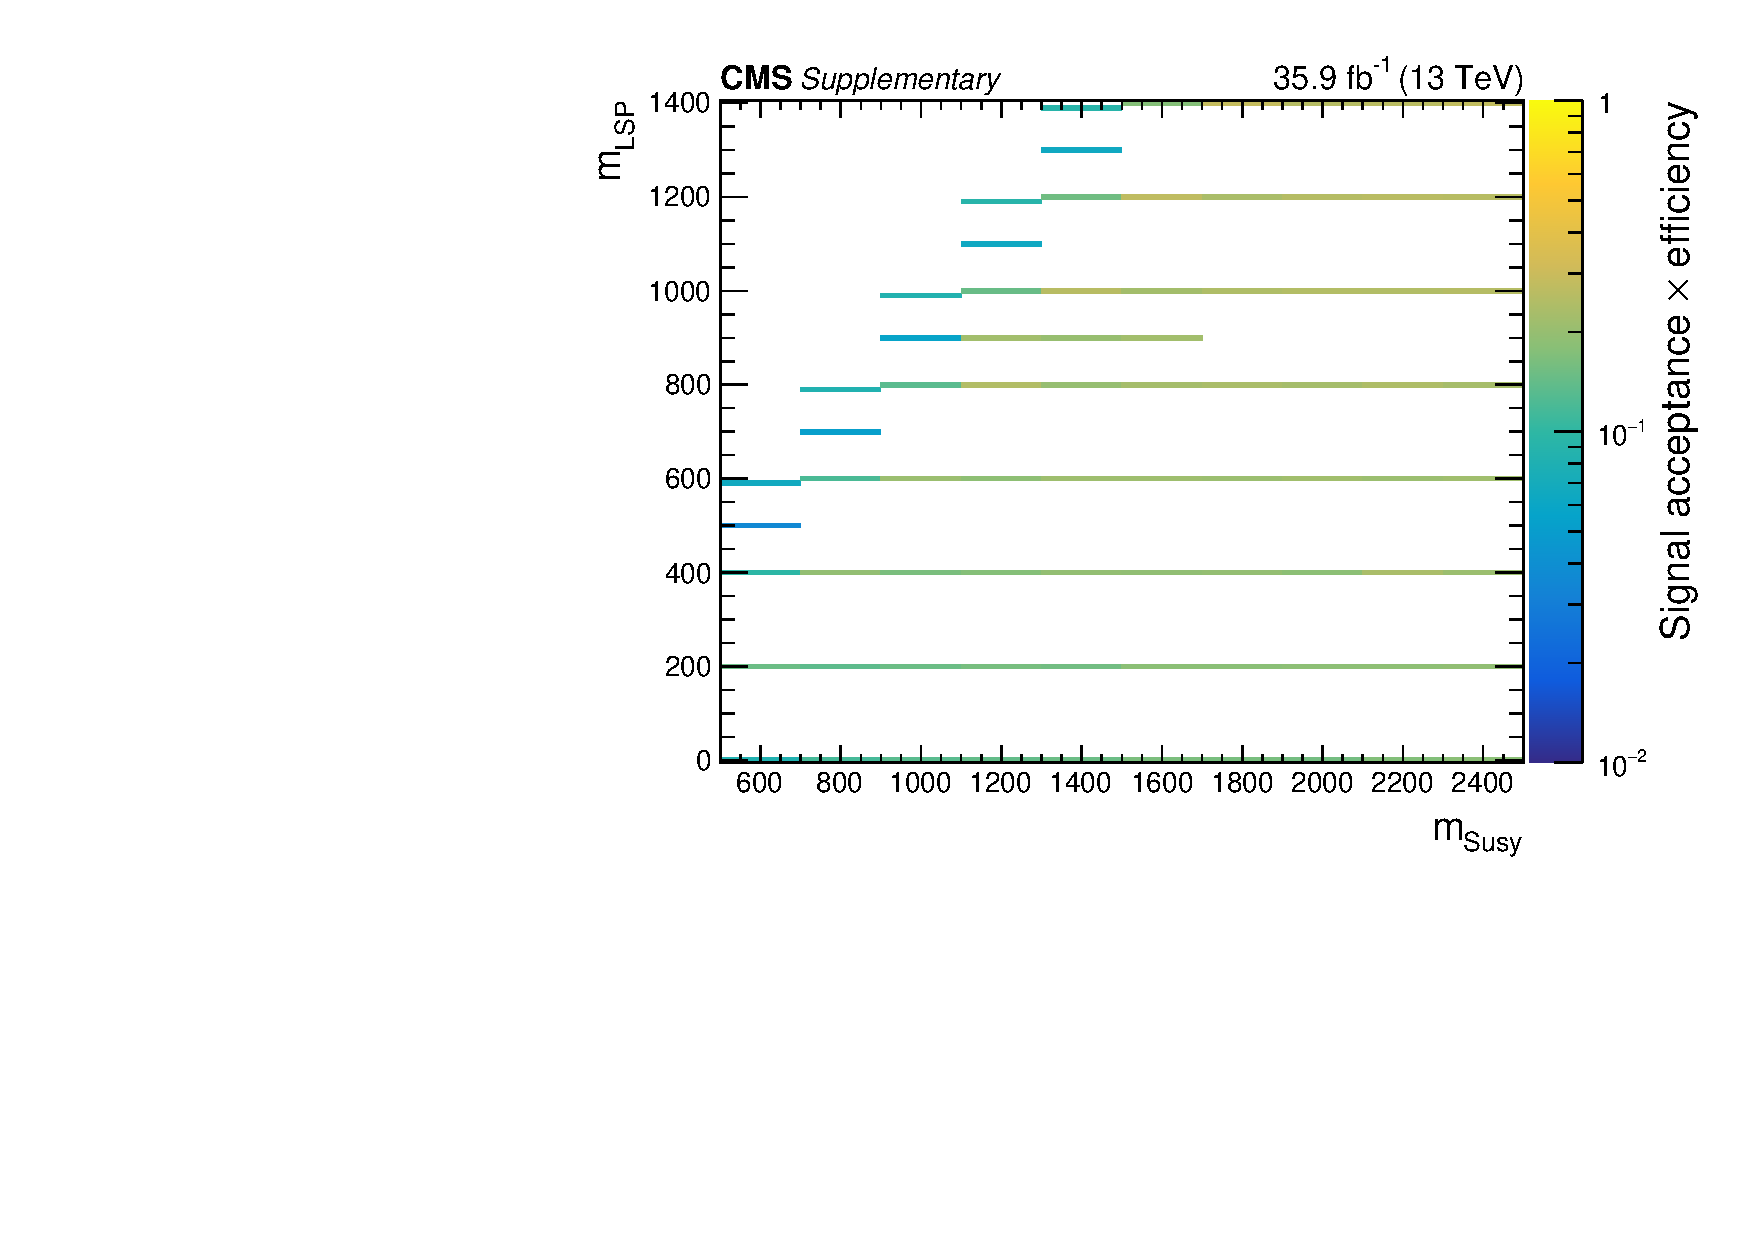
\includegraphics[width=0.45\textwidth]{figures/LLPResults/T1qqqqLL_ctau-10_effs}
            \label{fig:T1qqqqLL_eff}
        } ~~
        \subfigure[T1qqqqLL (\ctau = 10~mm): Most sensitive categories]{
            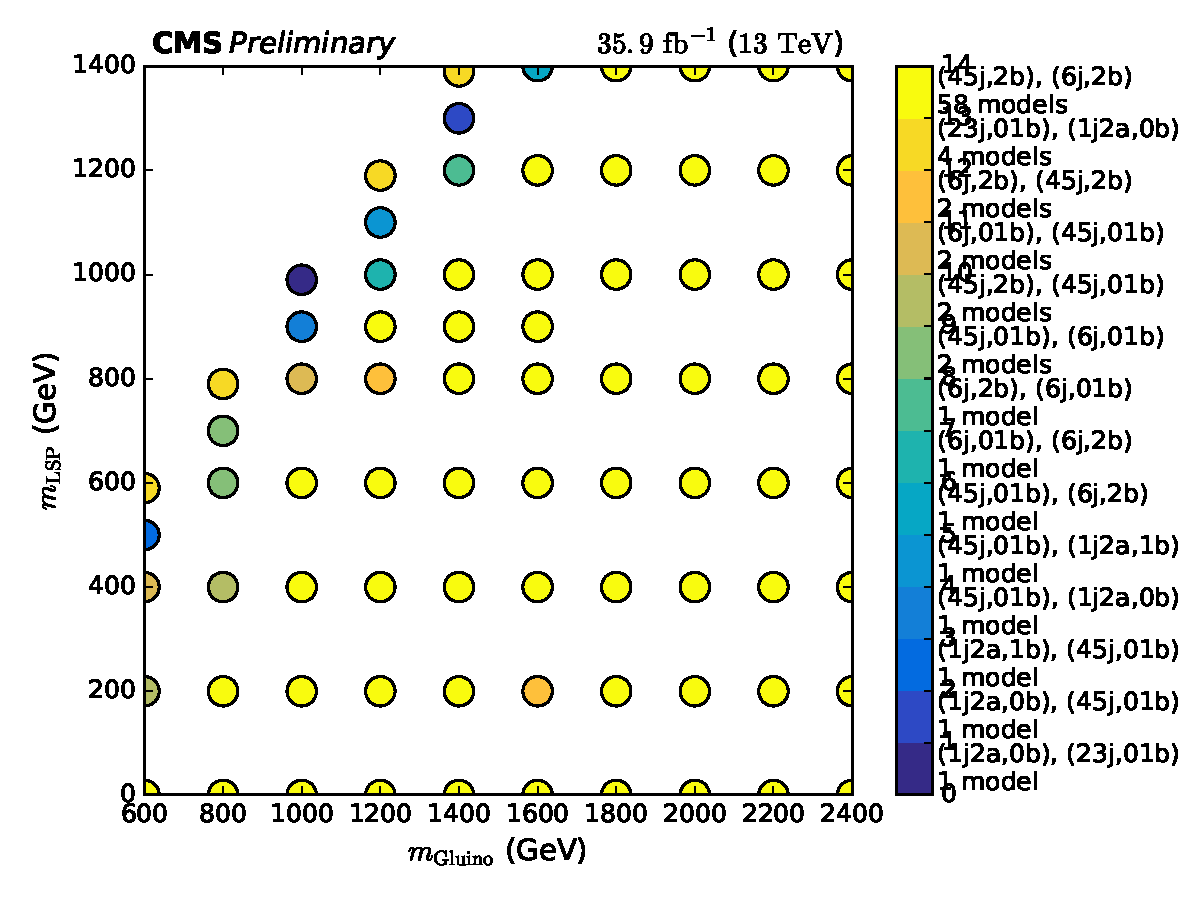
\includegraphics[width=0.45\textwidth]{figures/LLPResults/T1qqqqLL_ctau-10_bitMap}
            \label{fig:T1qqqqLL_bitMap}
        } \\
        %\subfigure[T1qqqqLL (\ctau = 1~mm): Significance scan]{
        %    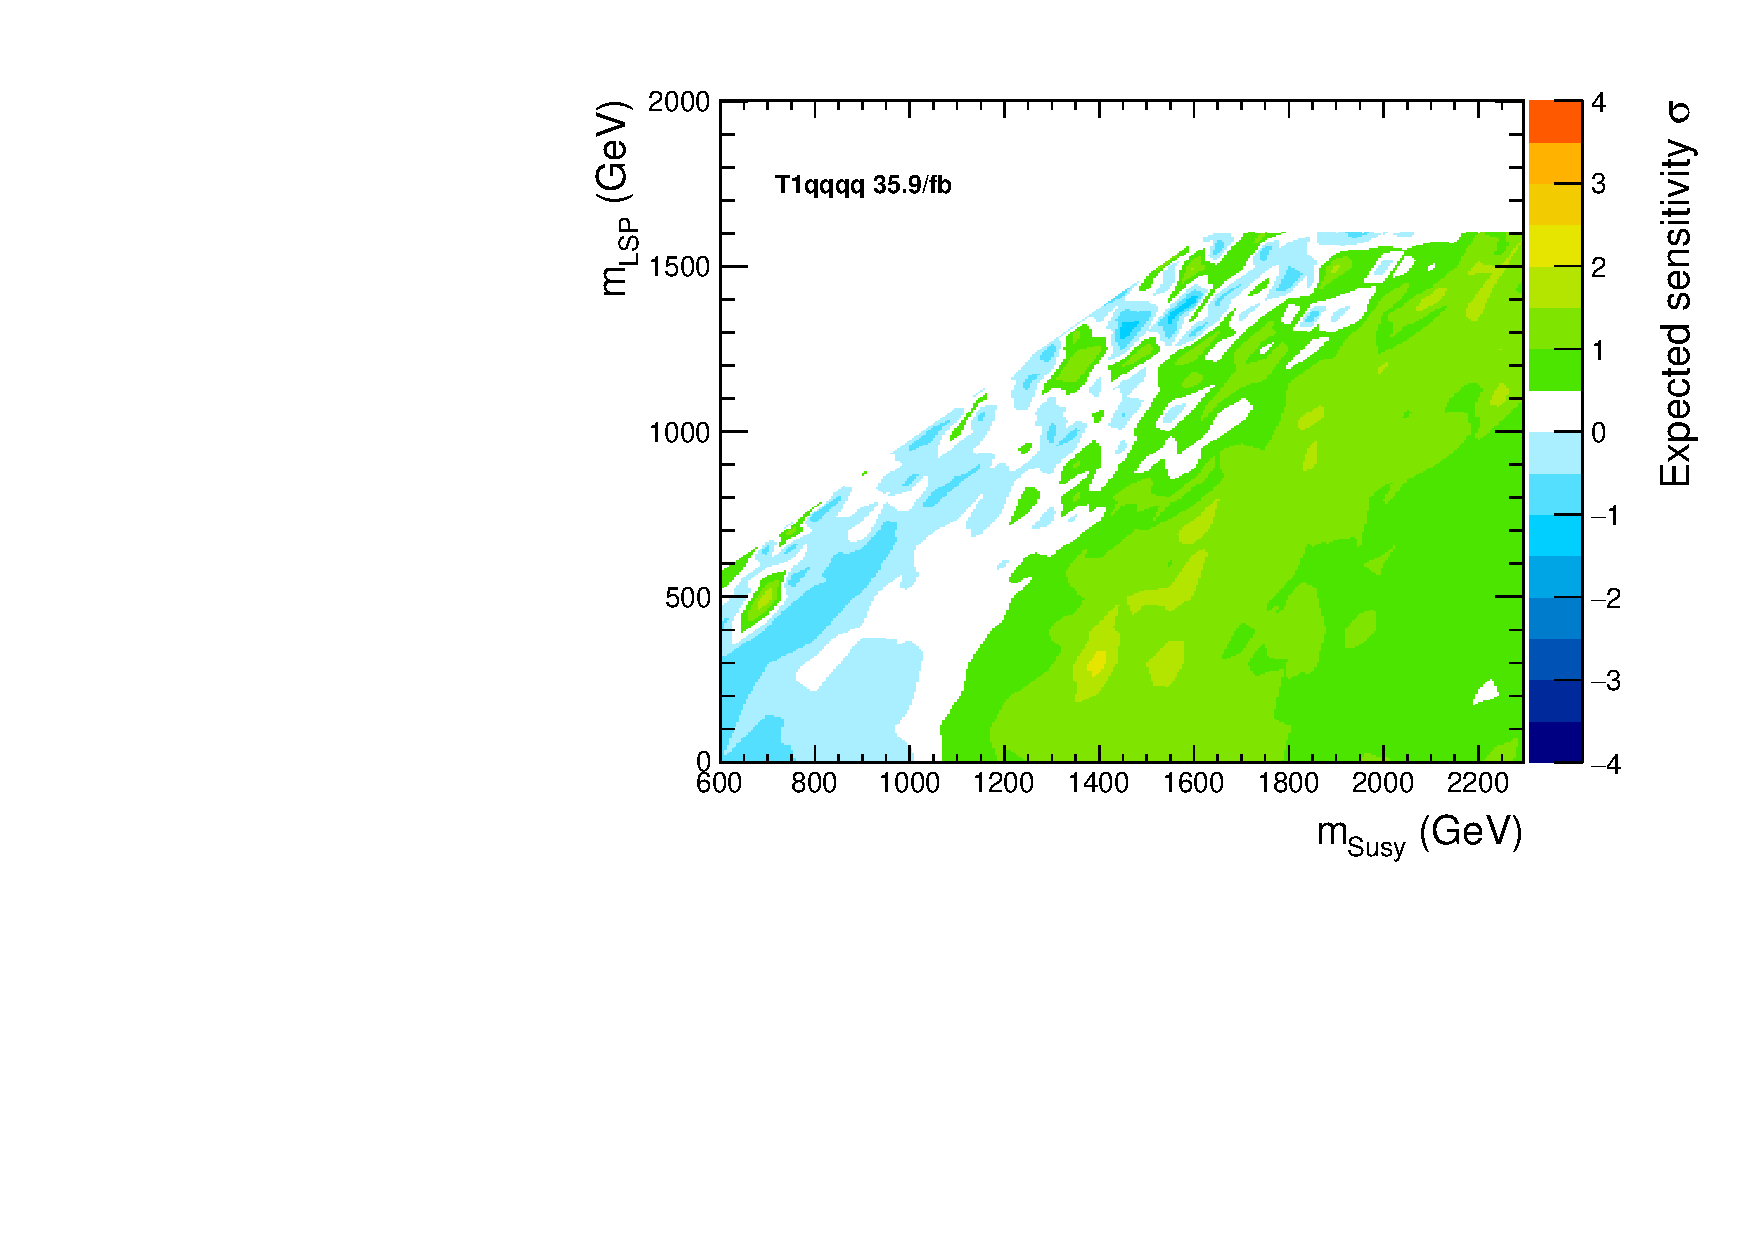
\includegraphics[width=0.45\linewidth]{figures/LLPResults/T1qqqqLL_ctau-1_signif}
        %    \label{fig:T1qqqqLL_signif}
        %} ~~
        \caption{Top: the 95\% C.L. observed upper limit on the cross section
            (histogram), with the expected (solid black line) observed
            (solid red line) exclusion contours. Left: signal acceptance
            including all jet categories. Right: graph showing the four
            most sensitive jet categories for each mass point.
            %Bottom: local observed significance scan.
        }
        \label{fig:T1qqqqLL:ctau-10}
    \end{center}
\end{figure}

\newpage
\begin{figure}[h!]
    \begin{center}
        \subfigure[T1qqqqLL (\ctau = 100~mm): Upper limit on the cross section in the mass plane]{
            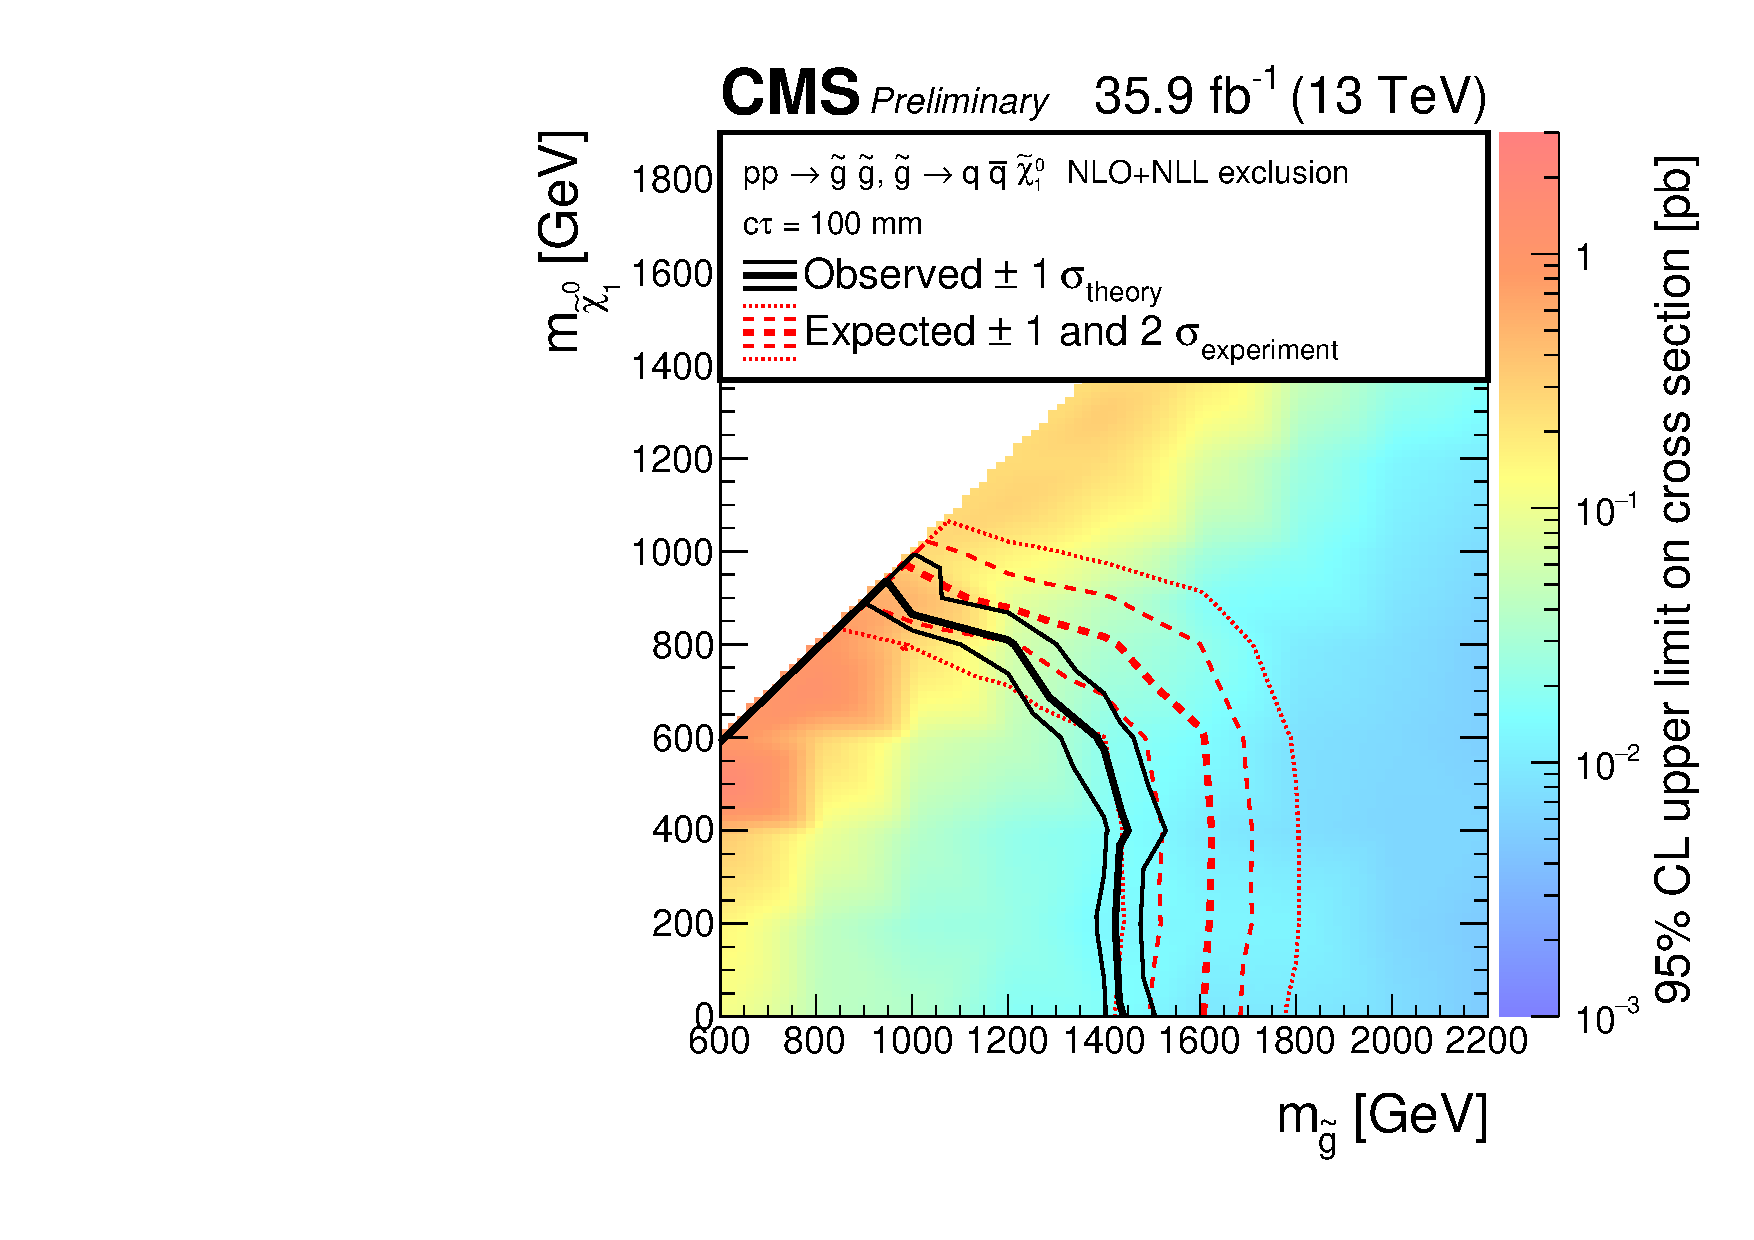
\includegraphics[width=0.6\textwidth]{figures/LLPResults/T1qqqqLL_ctau-100_XSEC}
            \label{fig:T1qqqqLL_excl}
        } \\
        \subfigure[T1qqqqLL (\ctau = 100~mm): $\epsilon_{sig}$]{
            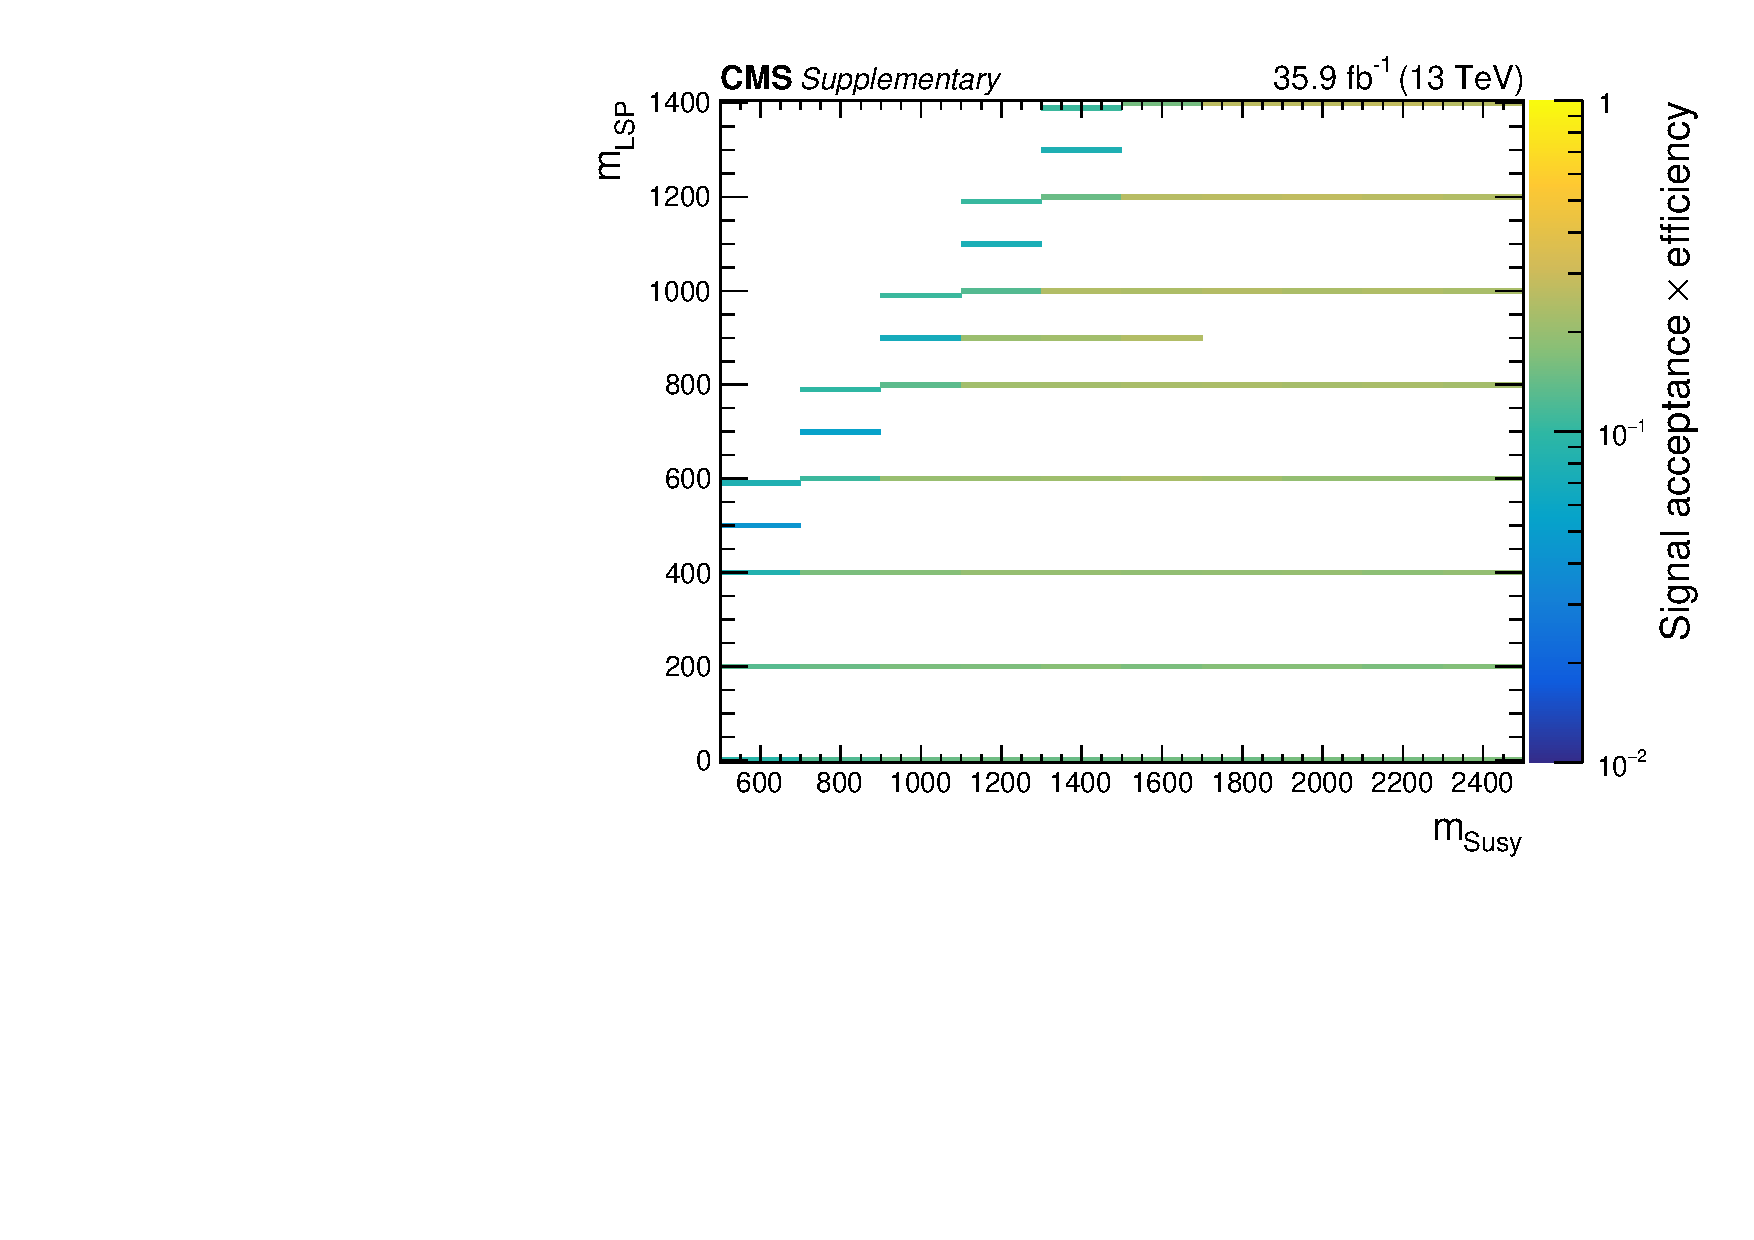
\includegraphics[width=0.45\textwidth]{figures/LLPResults/T1qqqqLL_ctau-100_effs}
            \label{fig:T1qqqqLL_eff}
        } ~~
        \subfigure[T1qqqqLL (\ctau = 100~mm): Most sensitive categories]{
            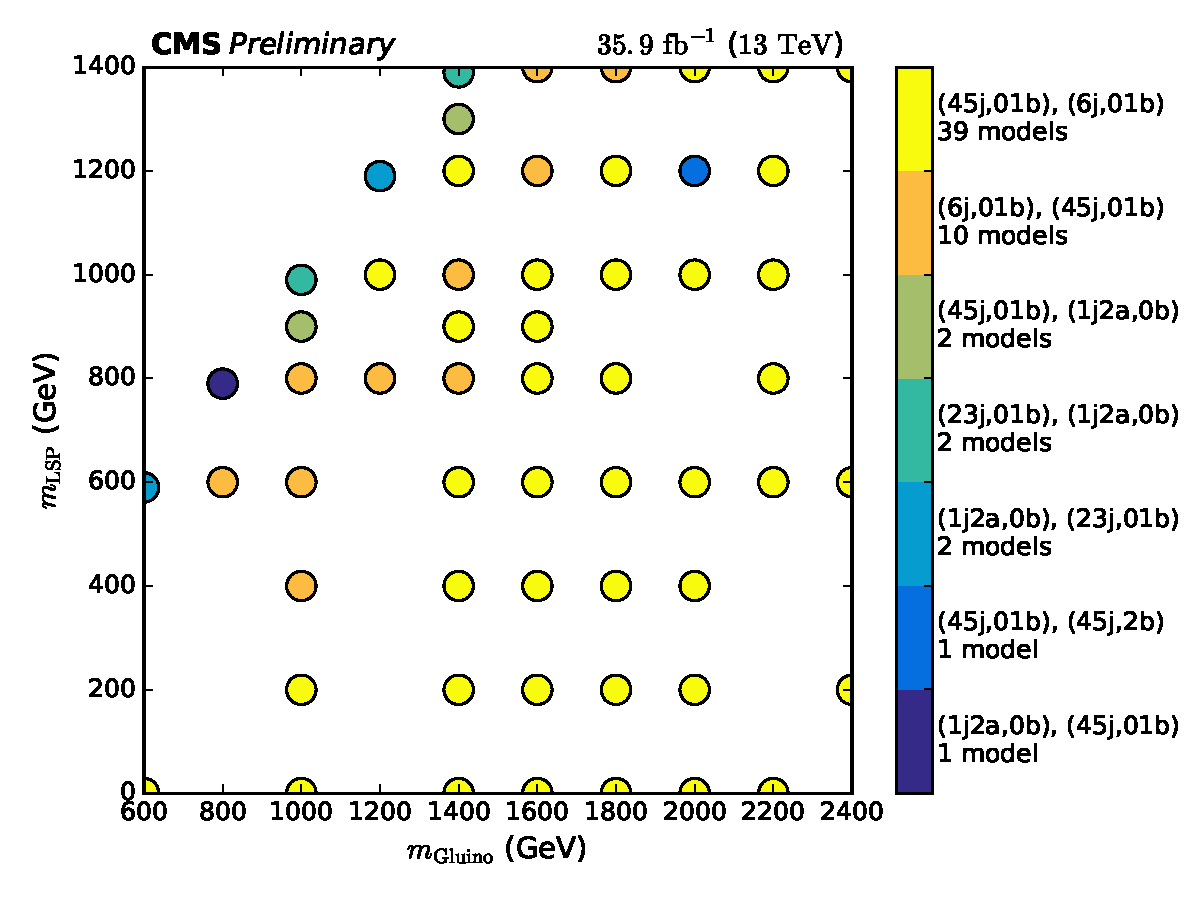
\includegraphics[width=0.45\textwidth]{figures/LLPResults/T1qqqqLL_ctau-100_bitMap}
            \label{fig:T1qqqqLL_bitMap}
        } \\
        %\subfigure[T1qqqqLL (\ctau = 1~mm): Significance scan]{
        %    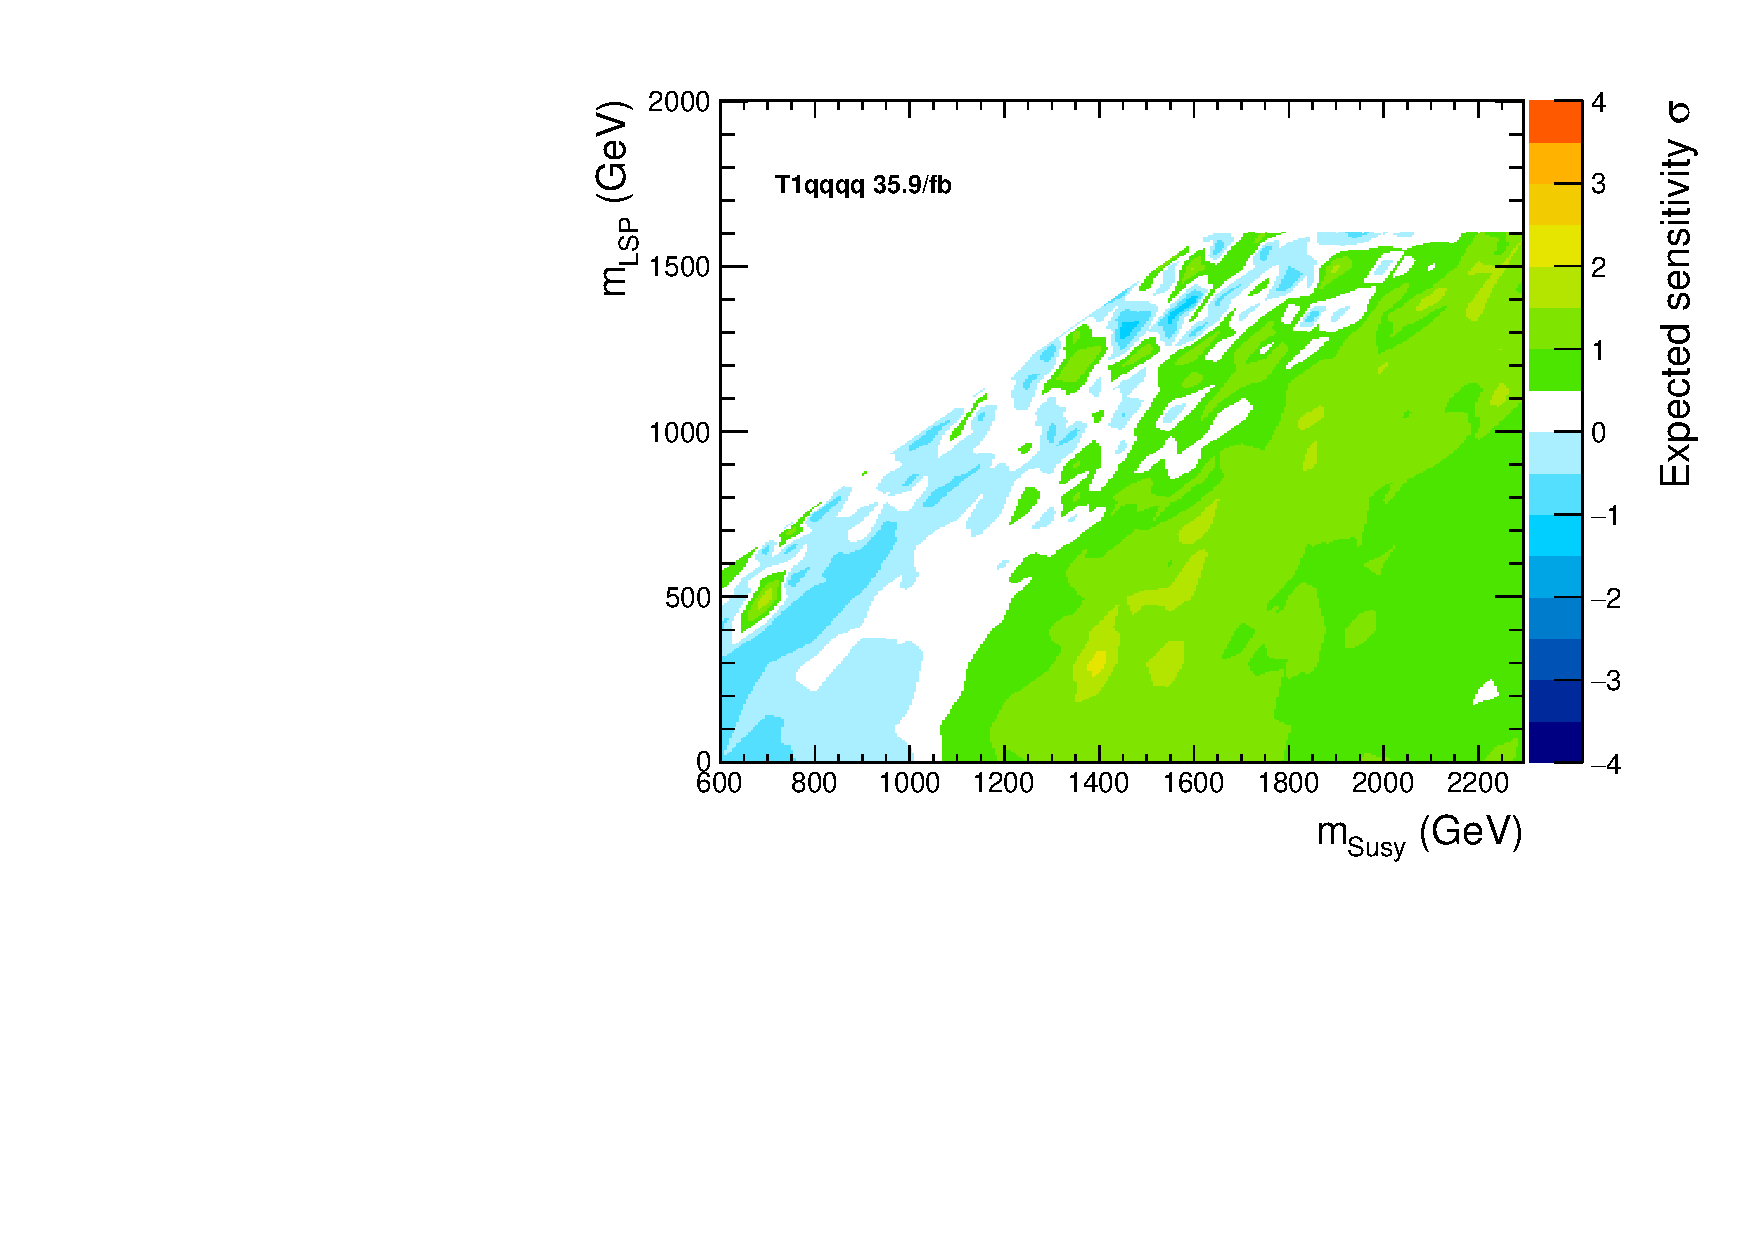
\includegraphics[width=0.45\linewidth]{figures/LLPResults/T1qqqqLL_ctau-1_signif}
        %    \label{fig:T1qqqqLL_signif}
        %} ~~
        \caption{Top: the 95\% C.L. observed upper limit on the cross section
            (histogram), with the expected (solid black line) observed
            (solid red line) exclusion contours. Left: signal acceptance
            including all jet categories. Right: graph showing the four
            most sensitive jet categories for each mass point.
            %Bottom: local observed significance scan.
        }
        \label{fig:T1qqqqLL:ctau-100}
    \end{center}
\end{figure}

\newpage
\begin{figure}[h!]
    \begin{center}
        \subfigure[T1qqqqLL (\ctau = 1000~mm): Upper limit on the cross section in the mass plane]{
            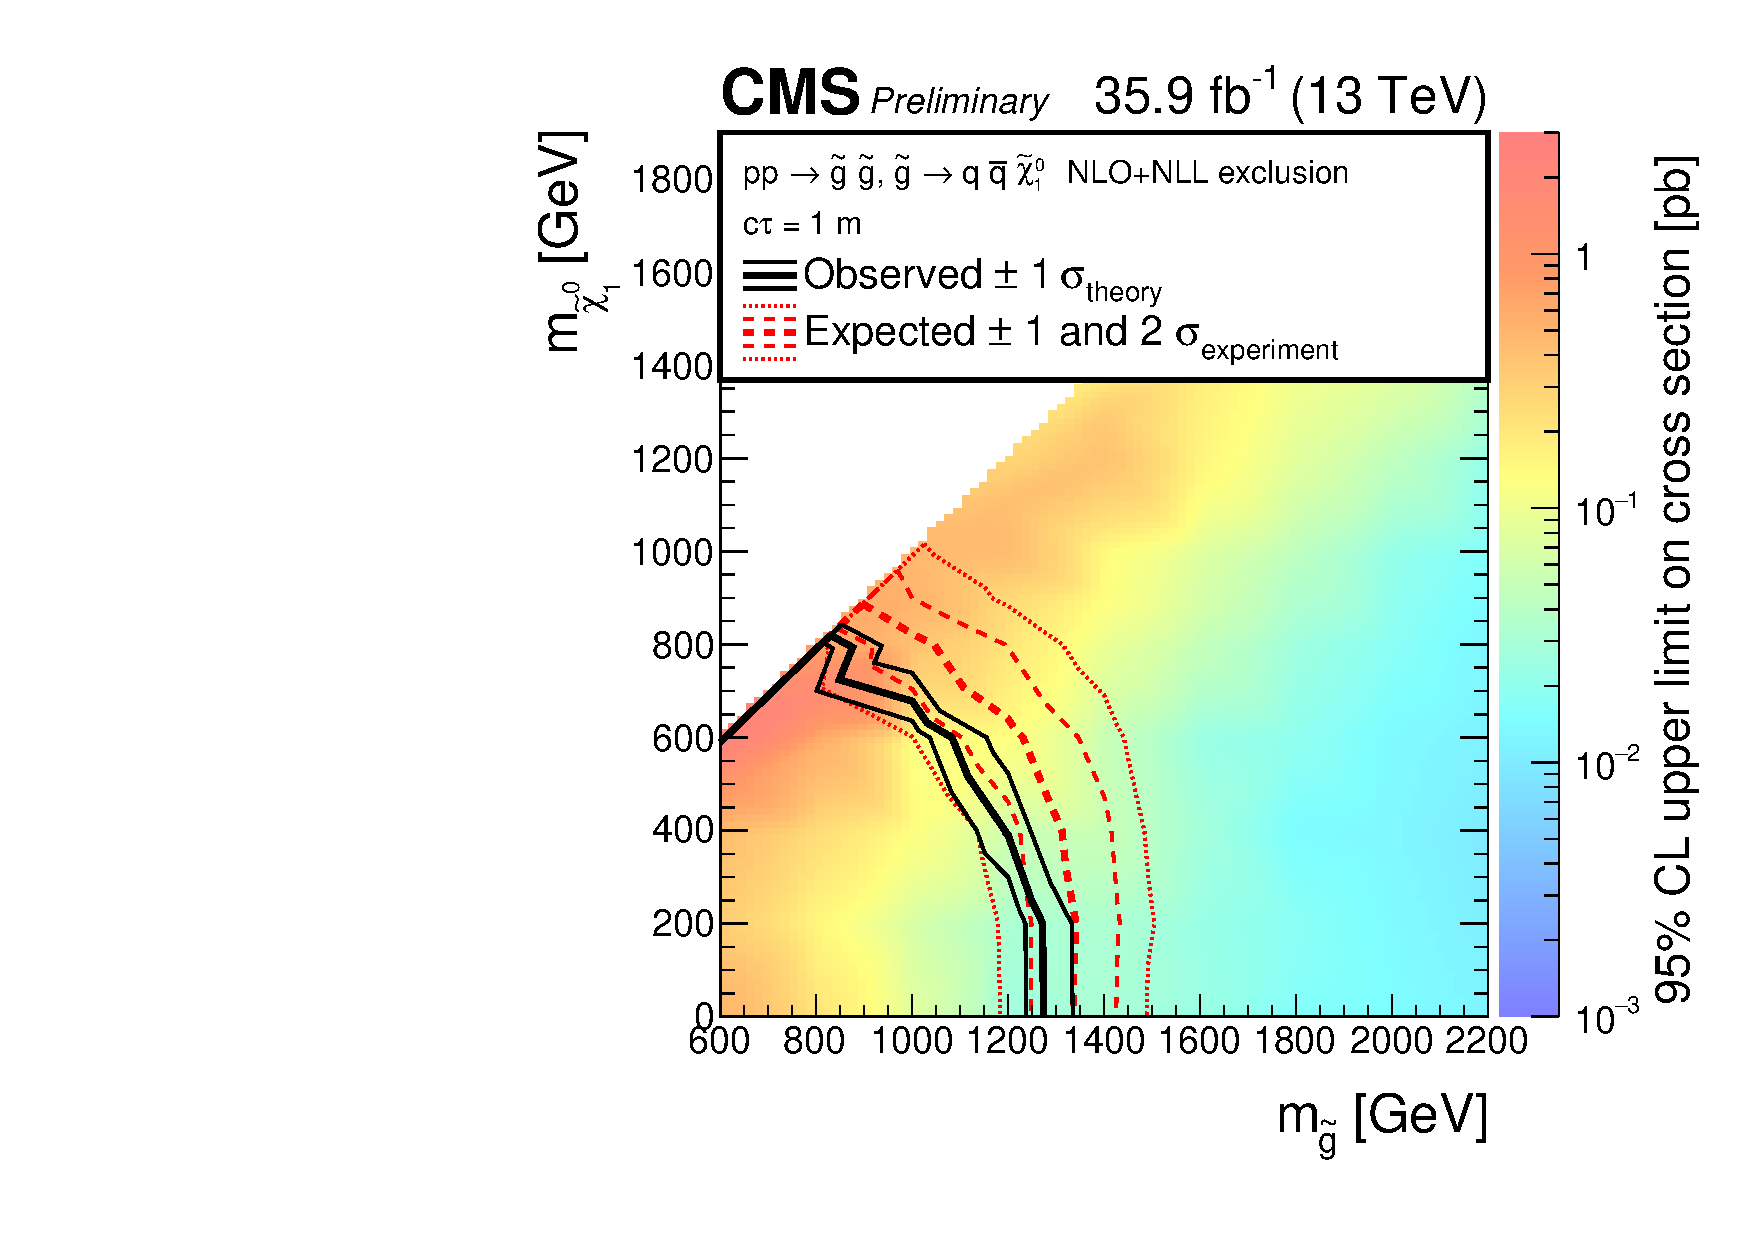
\includegraphics[width=0.6\textwidth]{figures/LLPResults/T1qqqqLL_ctau-1000_XSEC}
            \label{fig:T1qqqqLL_excl}
        } \\
        \subfigure[T1qqqqLL (\ctau = 1000~mm): $\epsilon_{sig}$]{
            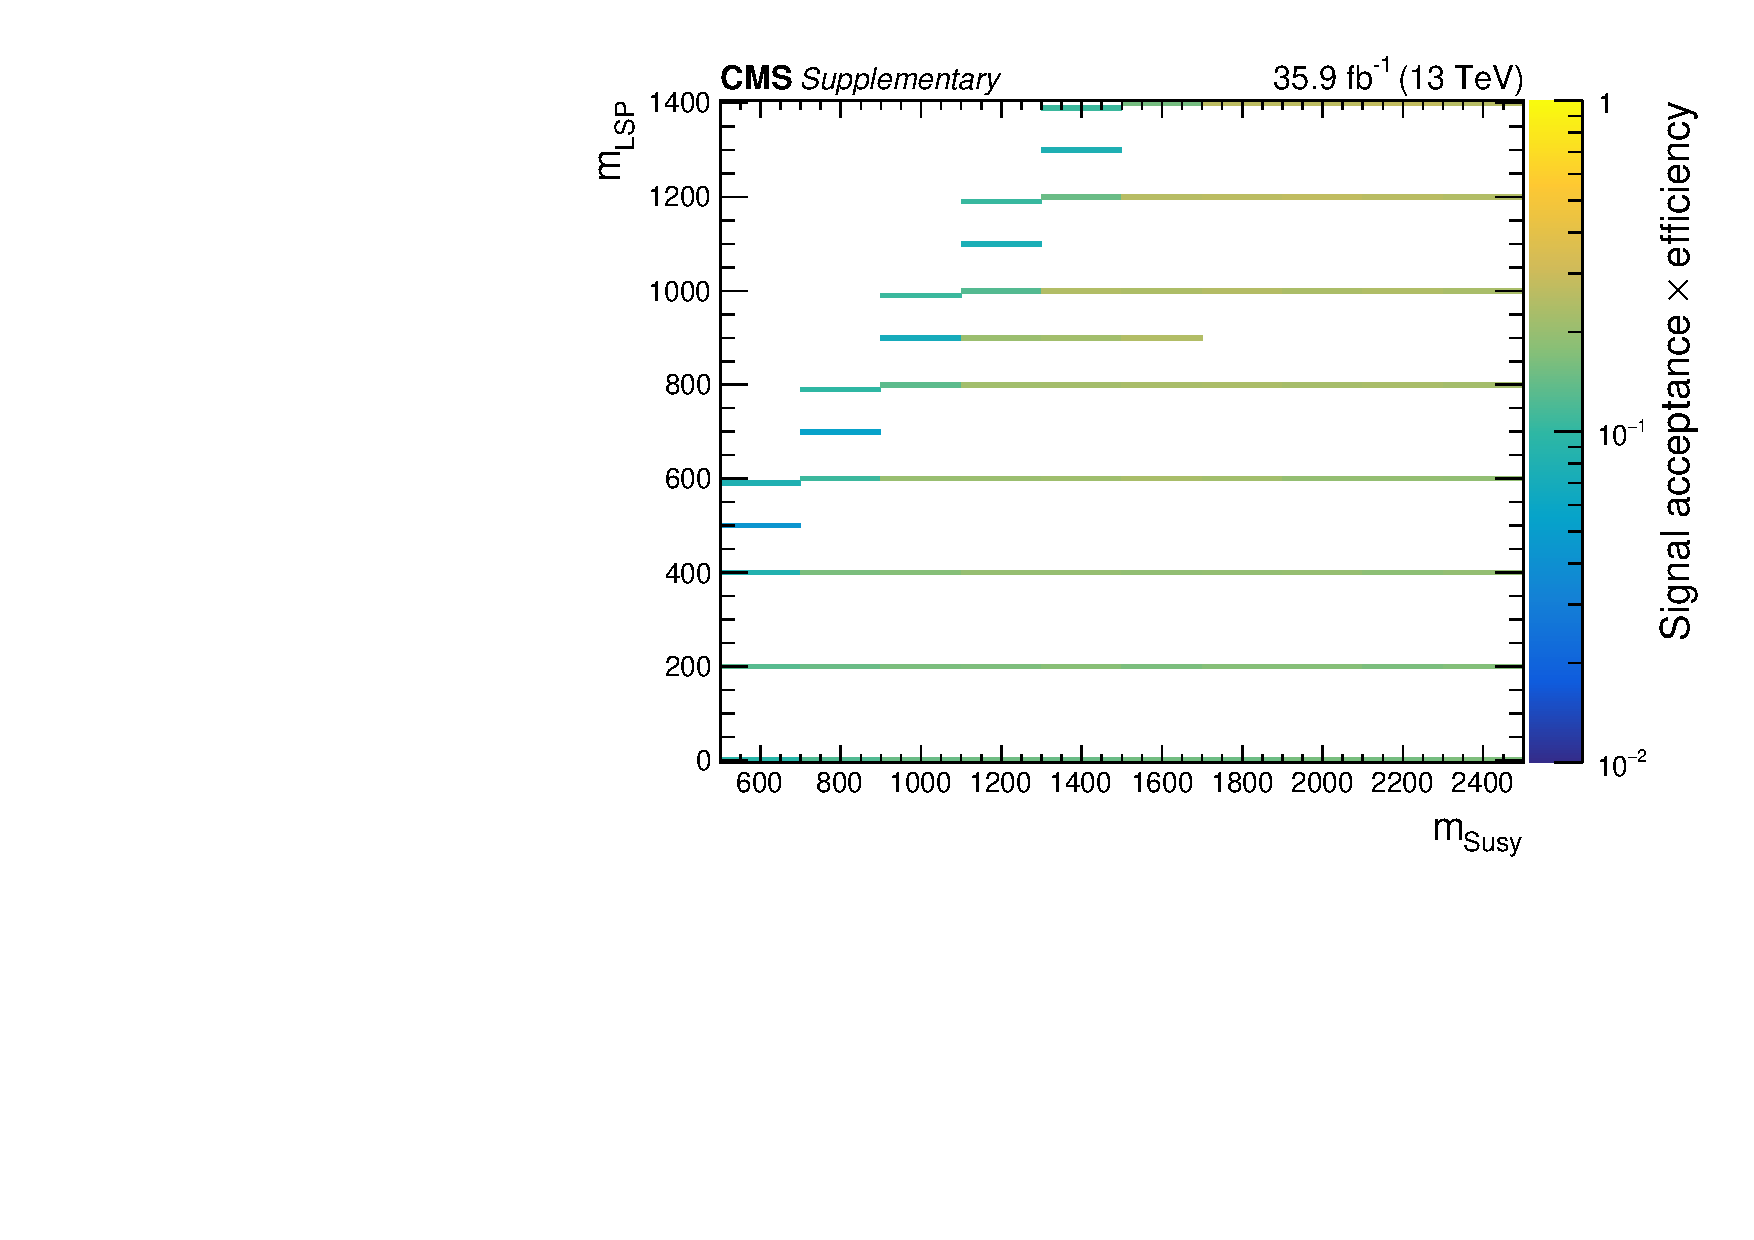
\includegraphics[width=0.45\textwidth]{figures/LLPResults/T1qqqqLL_ctau-1000_effs}
            \label{fig:T1qqqqLL_eff}
        } ~~
        \subfigure[T1qqqqLL (\ctau = 1000~mm): Most sensitive categories]{
            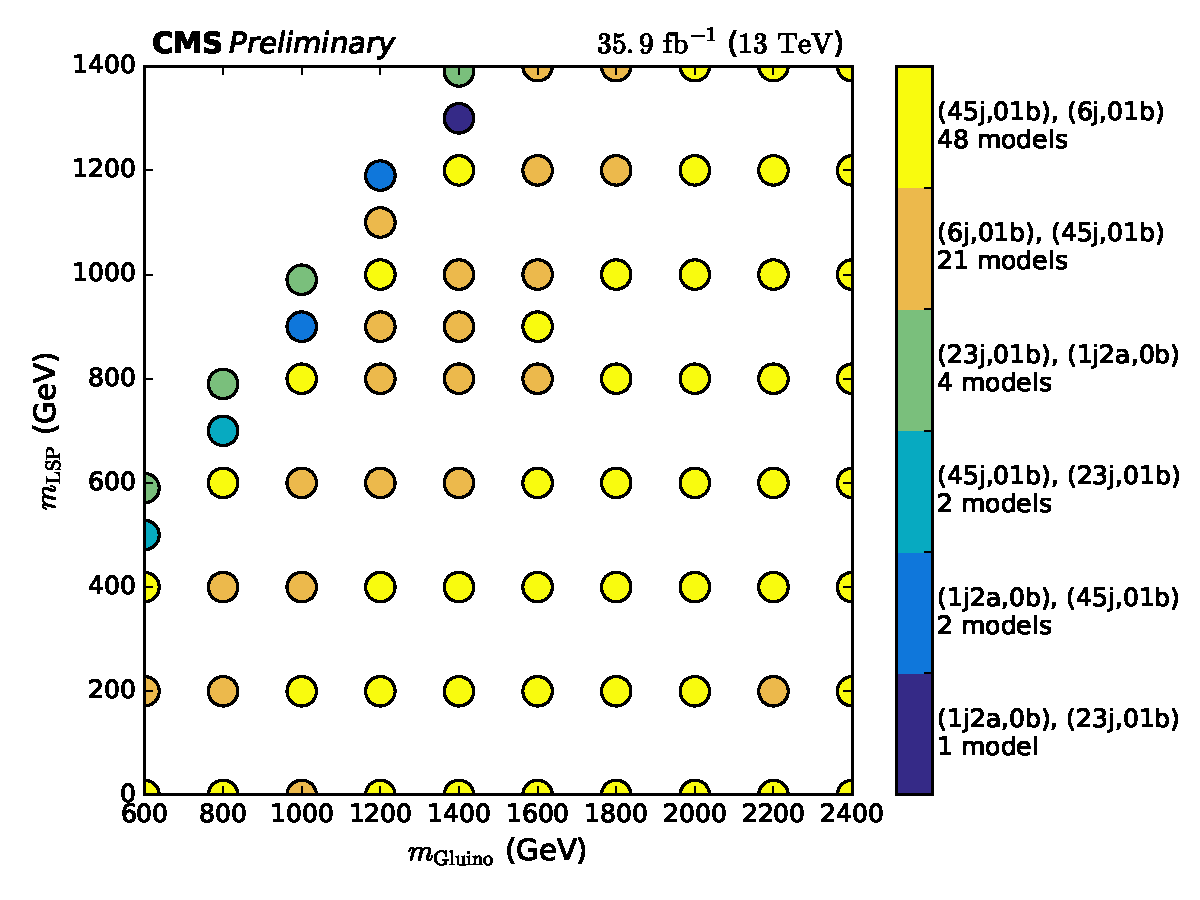
\includegraphics[width=0.45\textwidth]{figures/LLPResults/T1qqqqLL_ctau-1000_bitMap}
            \label{fig:T1qqqqLL_bitMap}
        } \\
        %\subfigure[T1qqqqLL (\ctau = 1~mm): Significance scan]{
        %    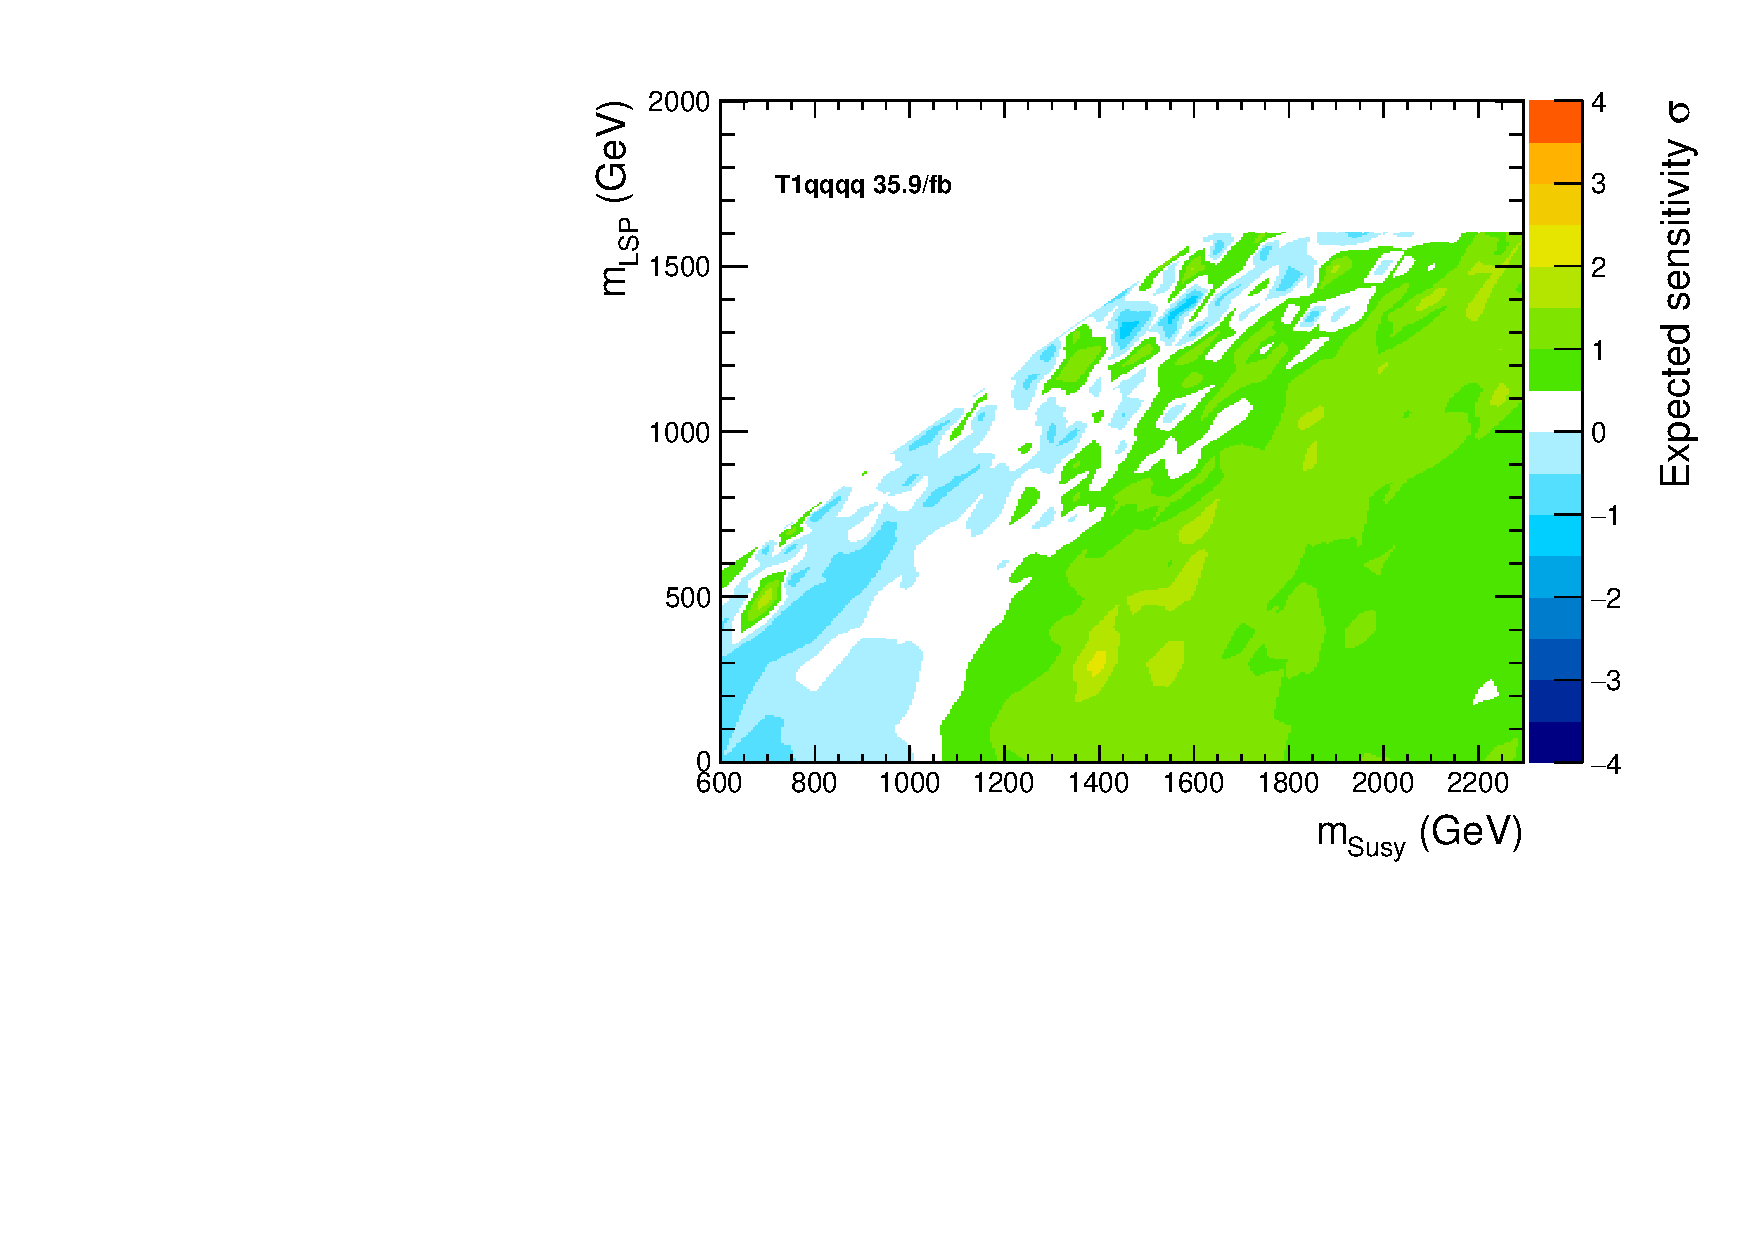
\includegraphics[width=0.45\linewidth]{figures/LLPResults/T1qqqqLL_ctau-1_signif}
        %    \label{fig:T1qqqqLL_signif}
        %} ~~
        \caption{Top: the 95\% C.L. observed upper limit on the cross section
            (histogram), with the expected (solid black line) observed
            (solid red line) exclusion contours. Left: signal acceptance
            including all jet categories. Right: graph showing the four
            most sensitive jet categories for each mass point.
            %Bottom: local observed significance scan.
        }
        \label{fig:T1qqqqLL:ctau-1000}
    \end{center}
\end{figure}

\newpage
\begin{figure}[h!]
    \begin{center}
        \subfigure[T1qqqqLL (\ctau = 10000~mm): Upper limit on the cross section in the mass plane]{
            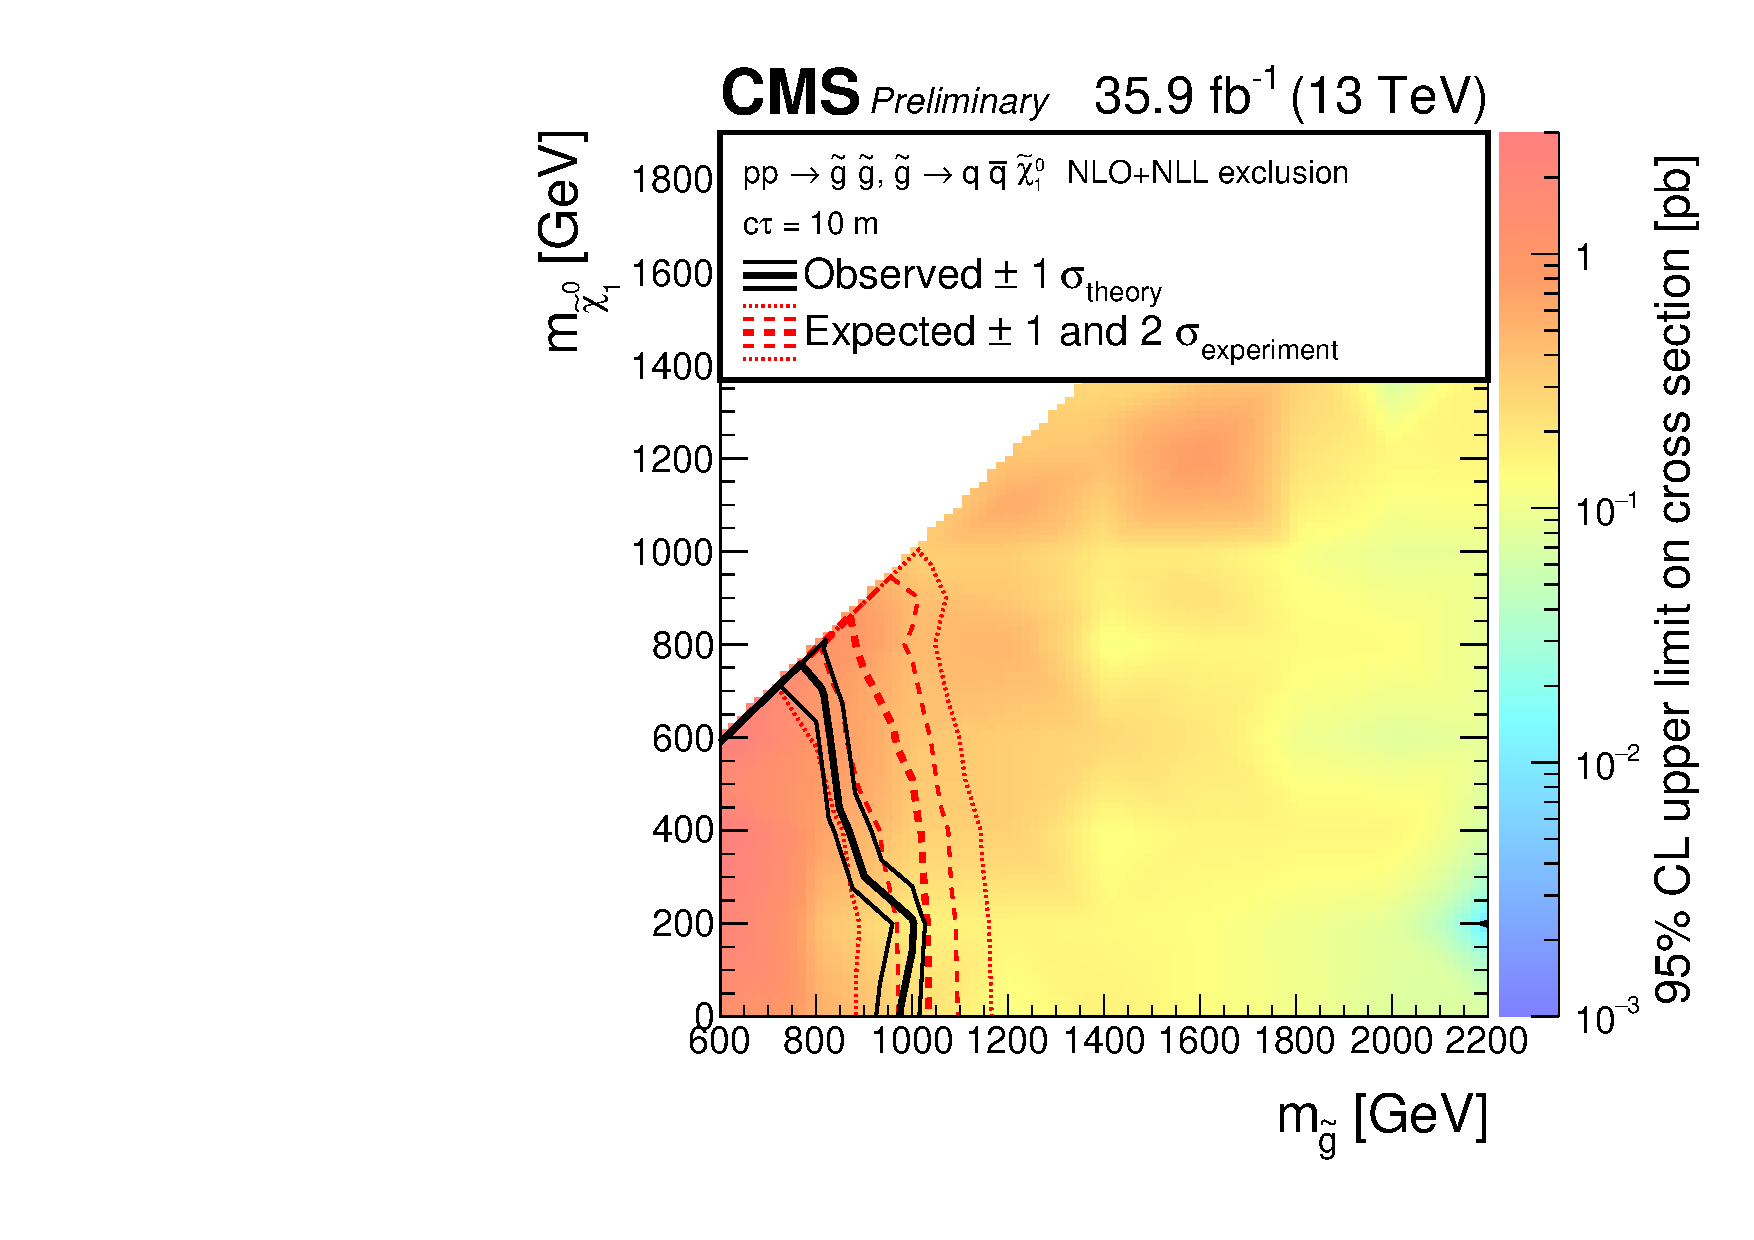
\includegraphics[width=0.6\textwidth]{figures/LLPResults/T1qqqqLL_ctau-10000_XSEC}
            \label{fig:T1qqqqLL_excl}
        } \\
        \subfigure[T1qqqqLL (\ctau = 10000~mm): $\epsilon_{sig}$]{
            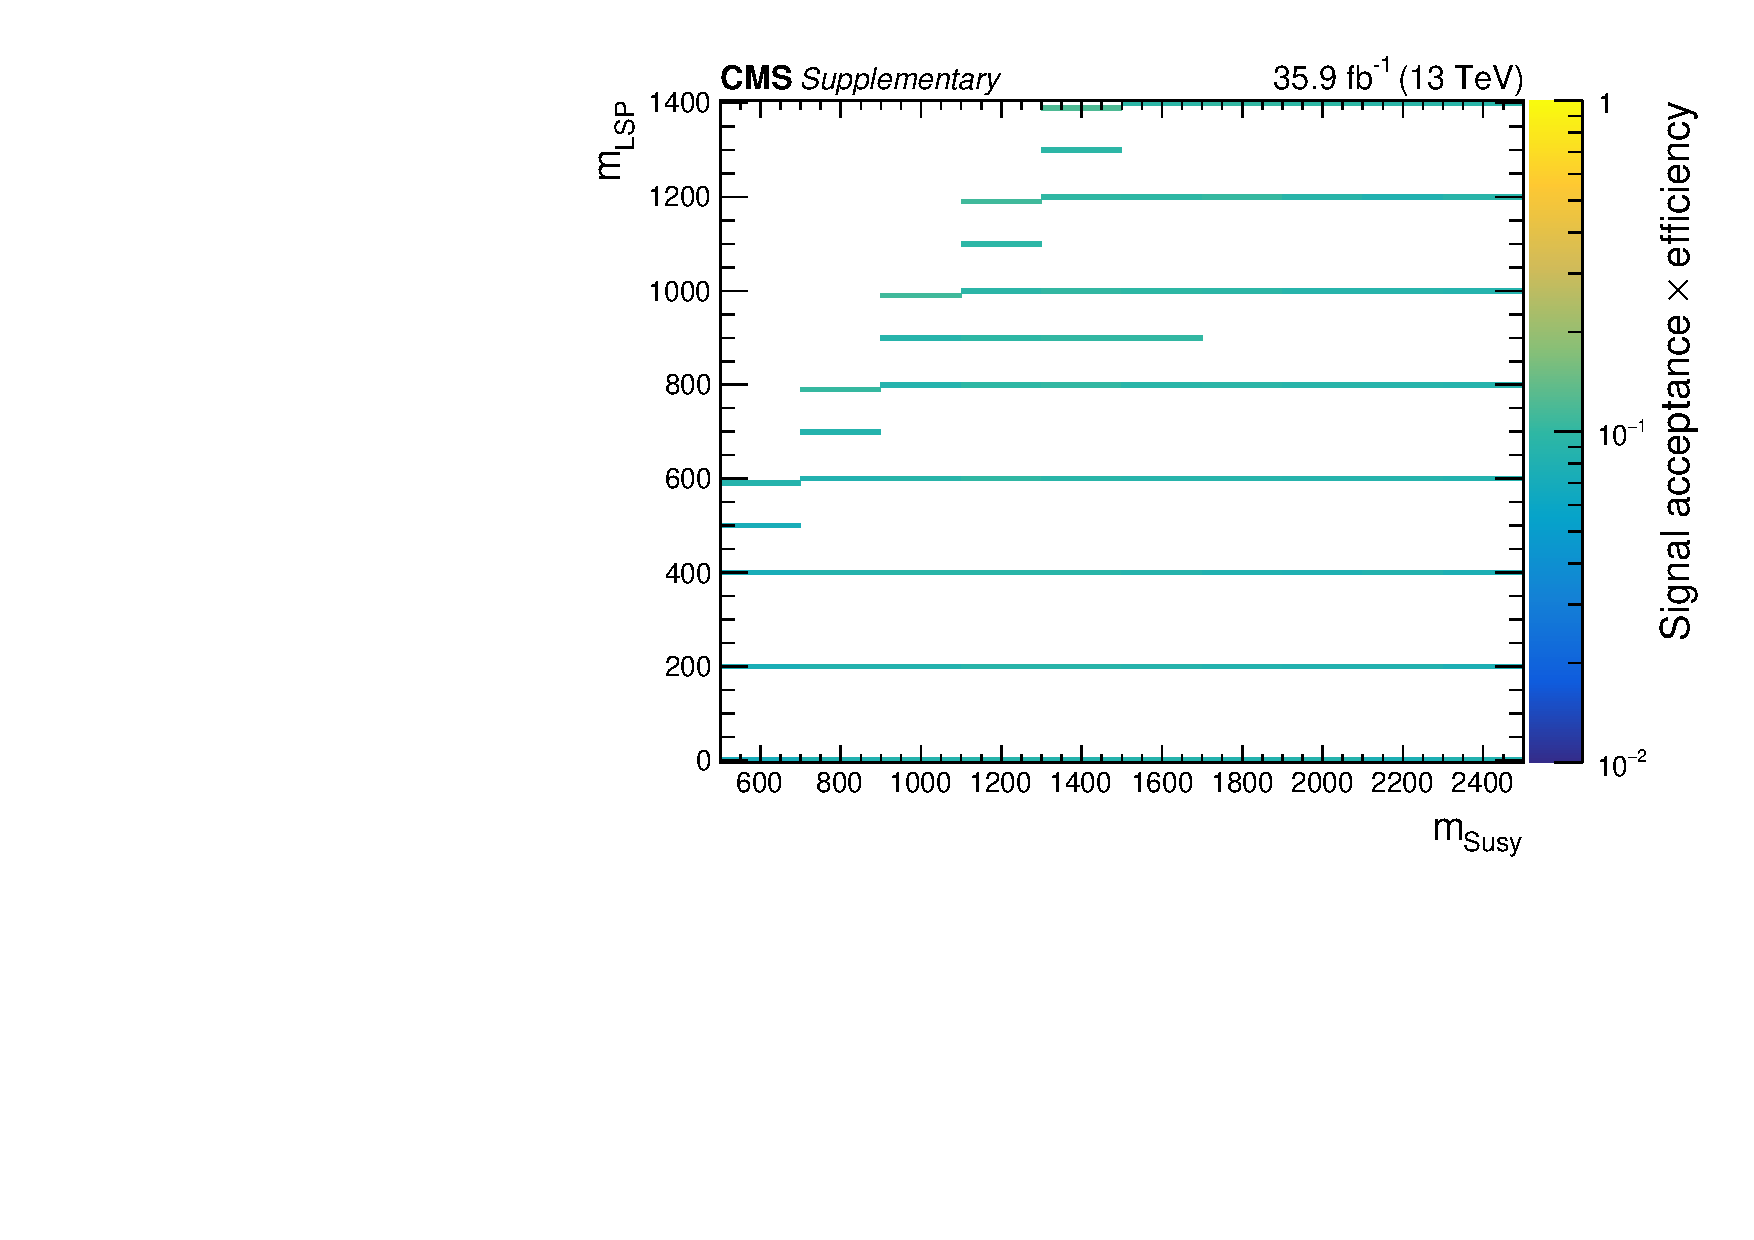
\includegraphics[width=0.45\textwidth]{figures/LLPResults/T1qqqqLL_ctau-10000_effs}
            \label{fig:T1qqqqLL_eff}
        } ~~
        \subfigure[T1qqqqLL (\ctau = 10000~mm): Most sensitive categories]{
            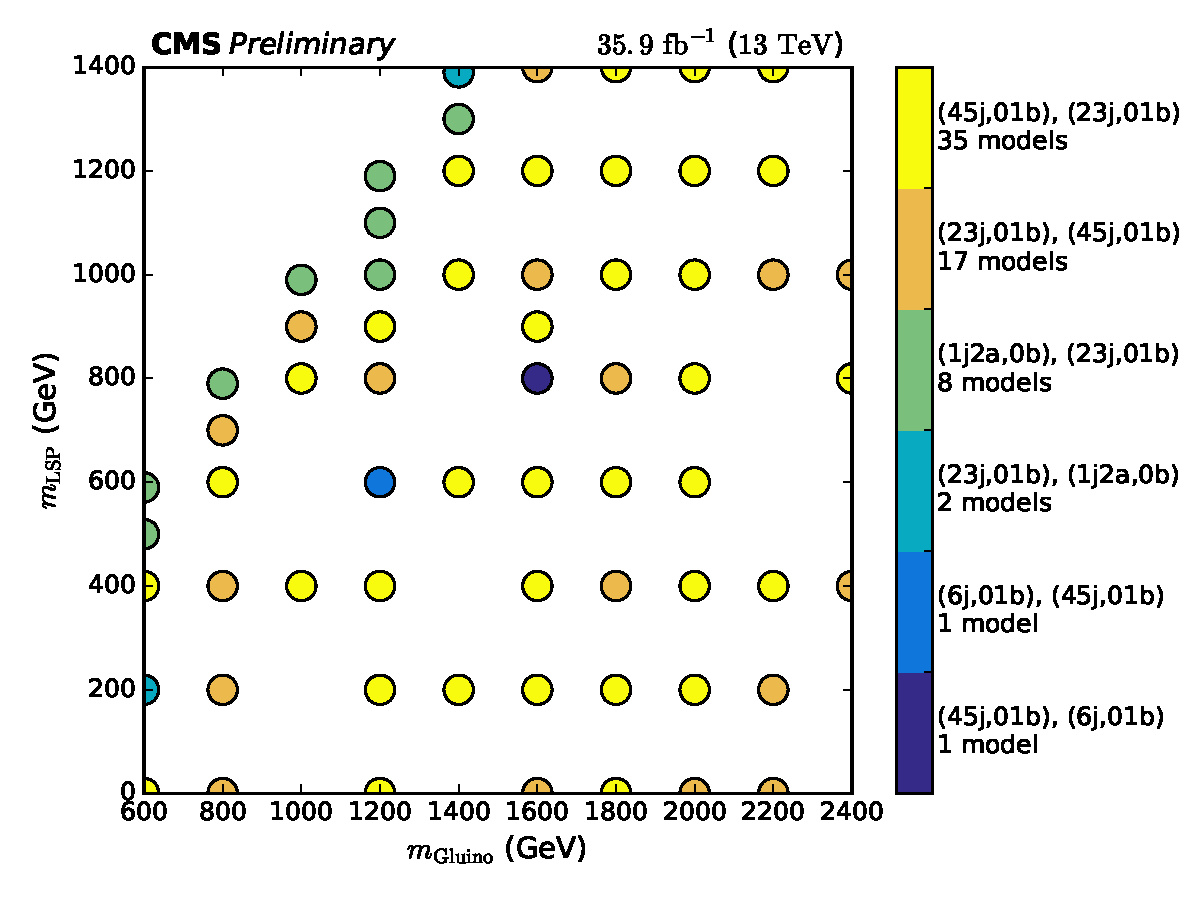
\includegraphics[width=0.45\textwidth]{figures/LLPResults/T1qqqqLL_ctau-10000_bitMap}
            \label{fig:T1qqqqLL_bitMap}
        } \\
        %\subfigure[T1qqqqLL (\ctau = 1~mm): Significance scan]{
        %    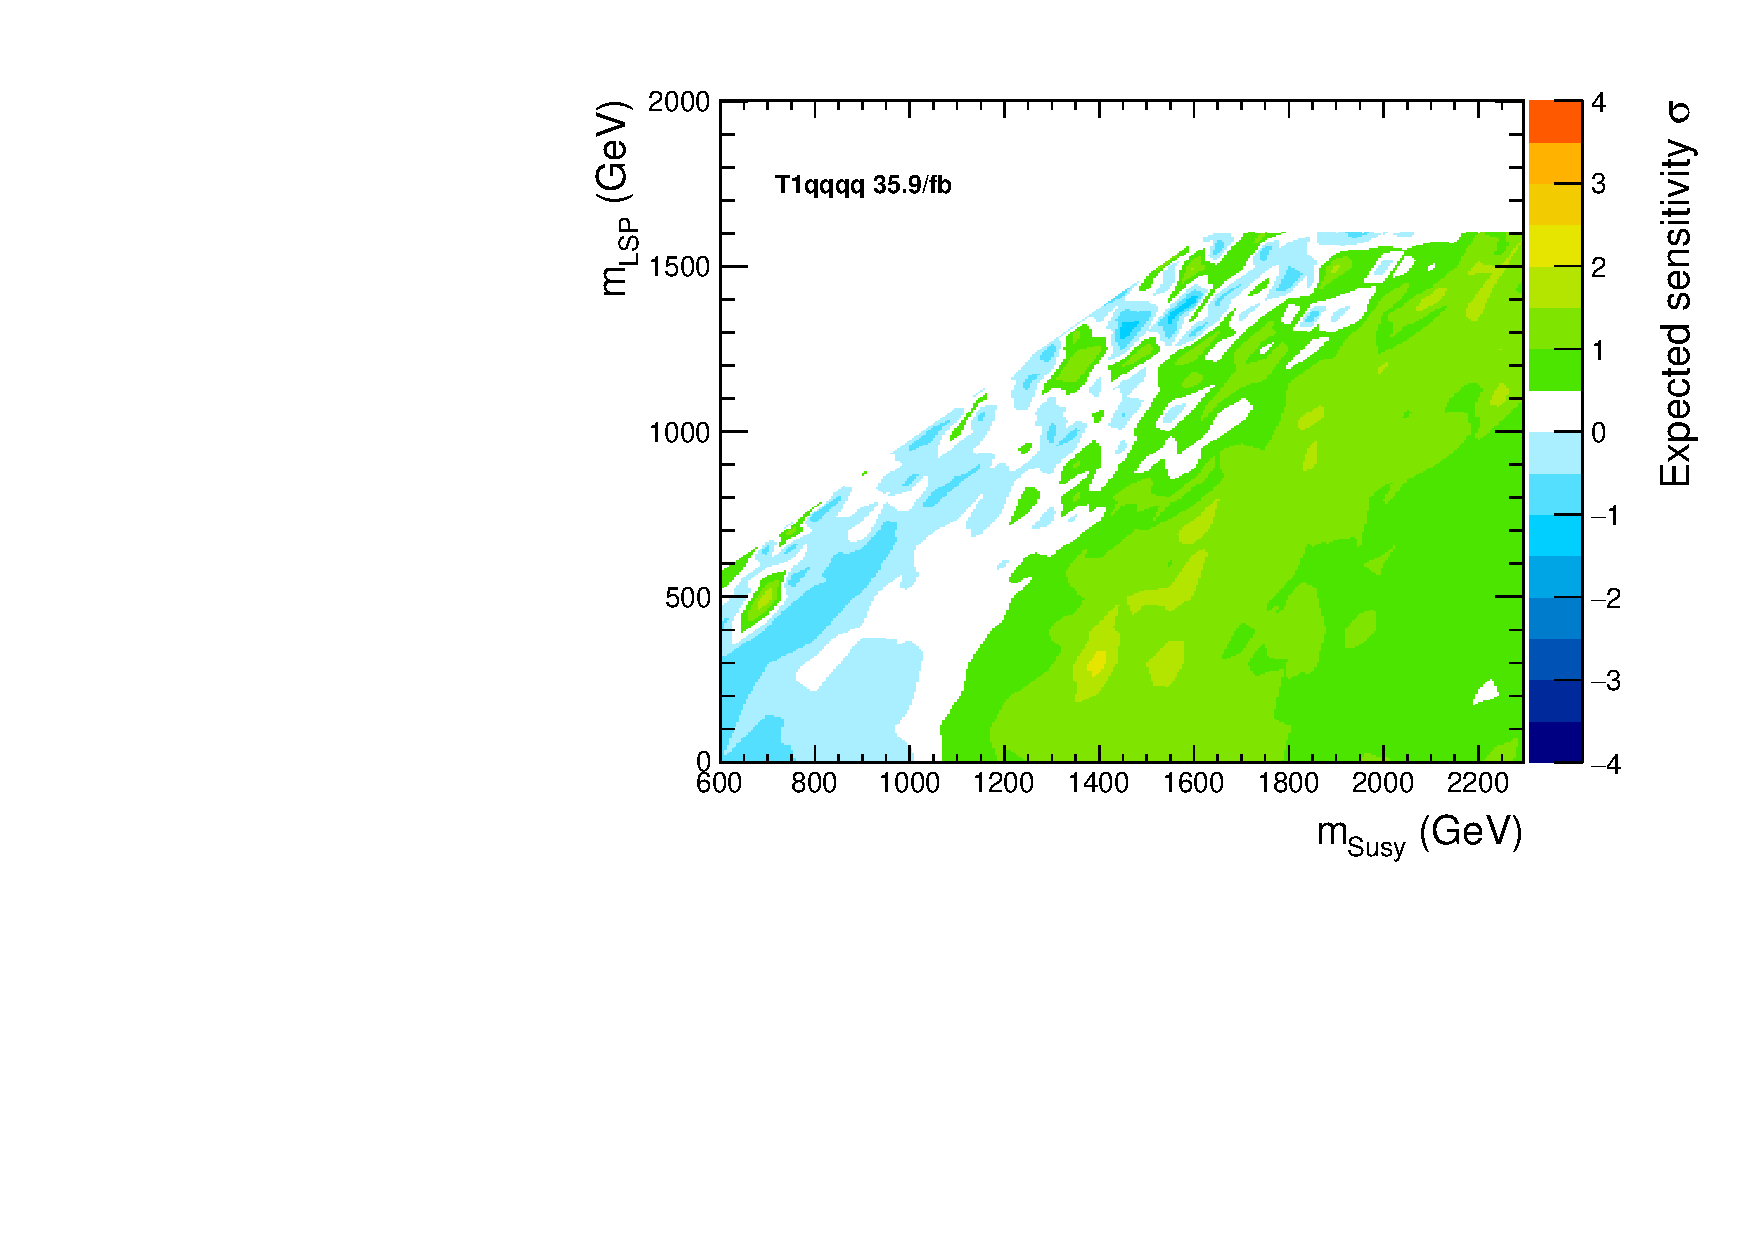
\includegraphics[width=0.45\linewidth]{figures/LLPResults/T1qqqqLL_ctau-1_signif}
        %    \label{fig:T1qqqqLL_signif}
        %} ~~
        \caption{Top: the 95\% C.L. observed upper limit on the cross section
            (histogram), with the expected (solid black line) observed
            (solid red line) exclusion contours. Left: signal acceptance
            including all jet categories. Right: graph showing the four
            most sensitive jet categories for each mass point.
            %Bottom: local observed significance scan.
        }
        \label{fig:T1qqqqLL:ctau-10000}
    \end{center}
\end{figure}

\newpage
\begin{figure}[h!]
    \begin{center}
        \subfigure[T1qqqqLL (\ctau = 100000~mm): Upper limit on the cross section in the mass plane]{
            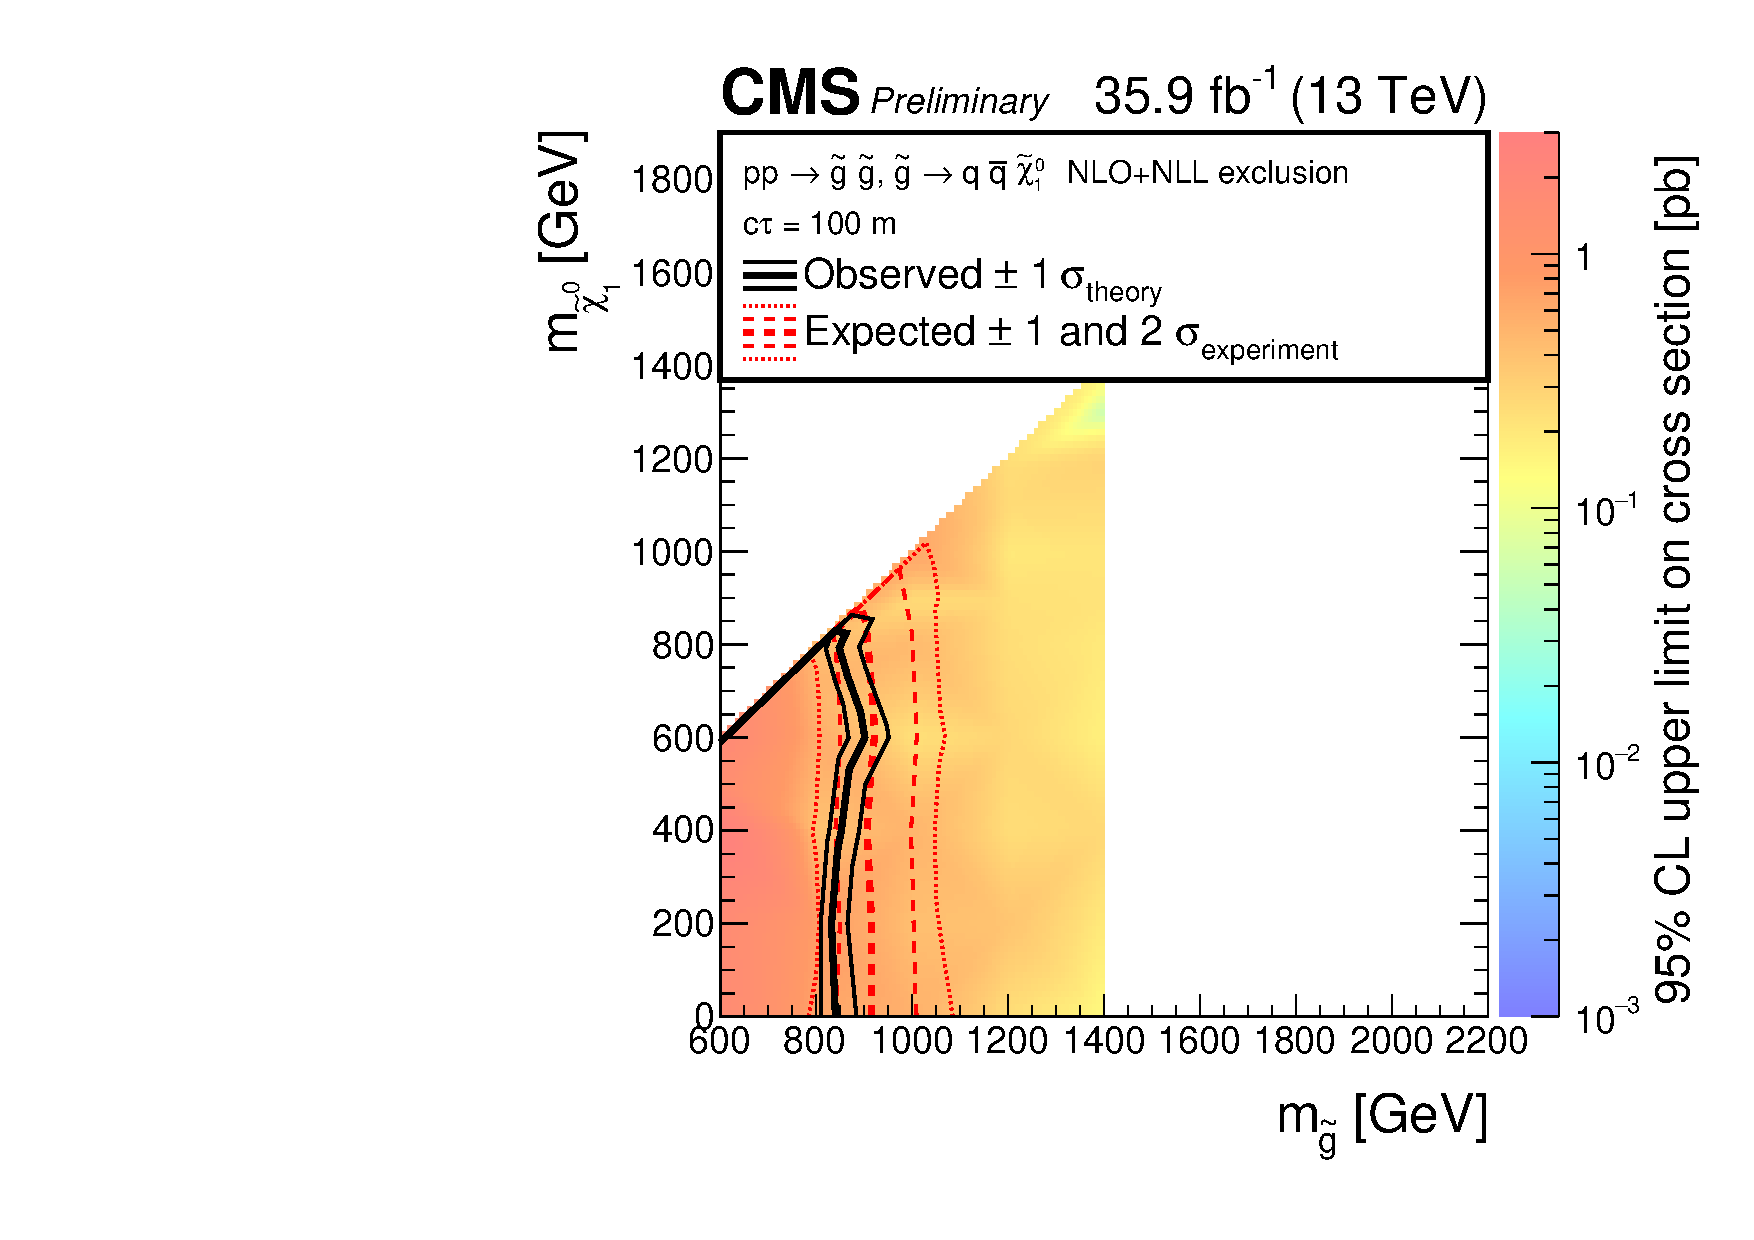
\includegraphics[width=0.6\textwidth]{figures/LLPResults/T1qqqqLL_ctau-100000_XSEC}
            \label{fig:T1qqqqLL_excl}
        } \\
        \subfigure[T1qqqqLL (\ctau = 100000~mm): $\epsilon_{sig}$]{
            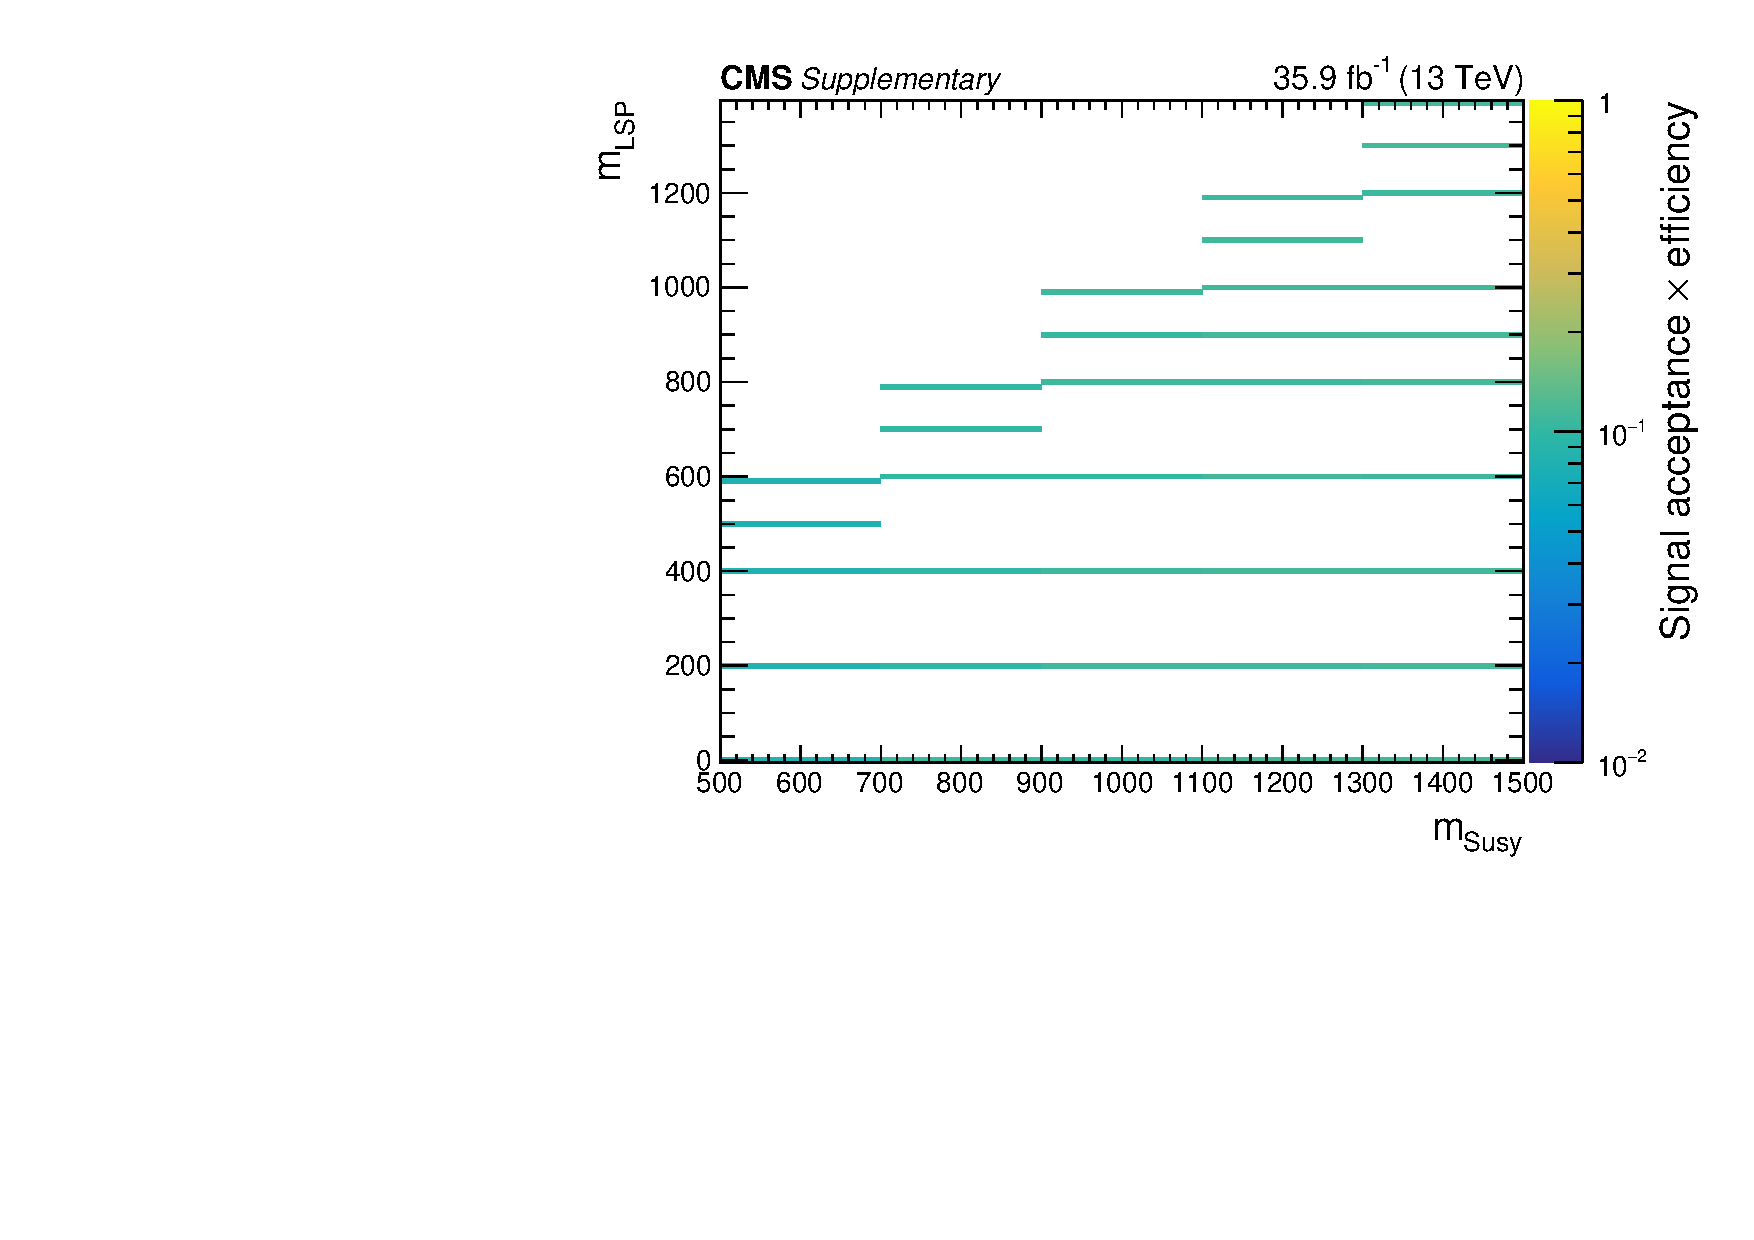
\includegraphics[width=0.45\textwidth]{figures/LLPResults/T1qqqqLL_ctau-100000_effs}
            \label{fig:T1qqqqLL_eff}
        } ~~
        \subfigure[T1qqqqLL (\ctau = 100000~mm): Most sensitive categories]{
            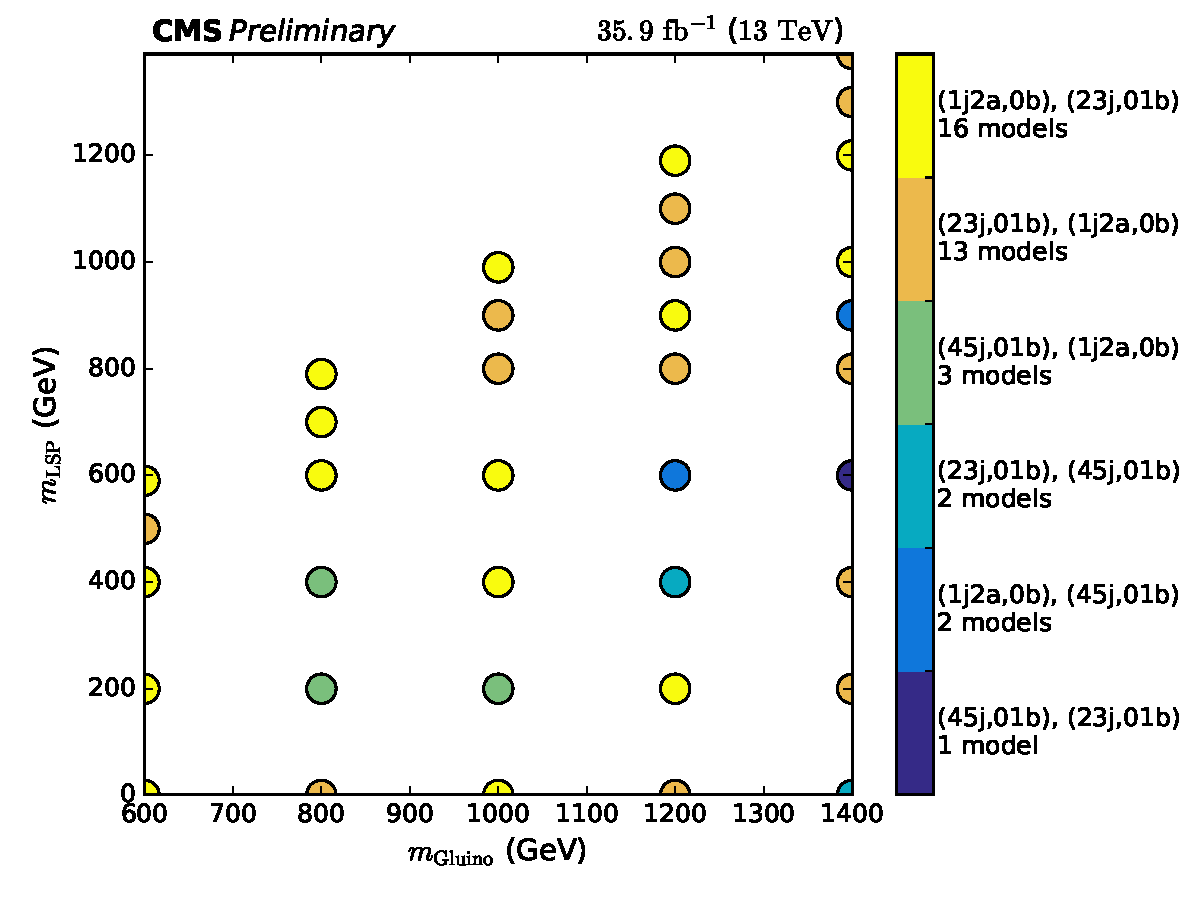
\includegraphics[width=0.45\textwidth]{figures/LLPResults/T1qqqqLL_ctau-100000_bitMap}
            \label{fig:T1qqqqLL_bitMap}
        } \\
        %\subfigure[T1qqqqLL (\ctau = 1~mm): Significance scan]{
        %    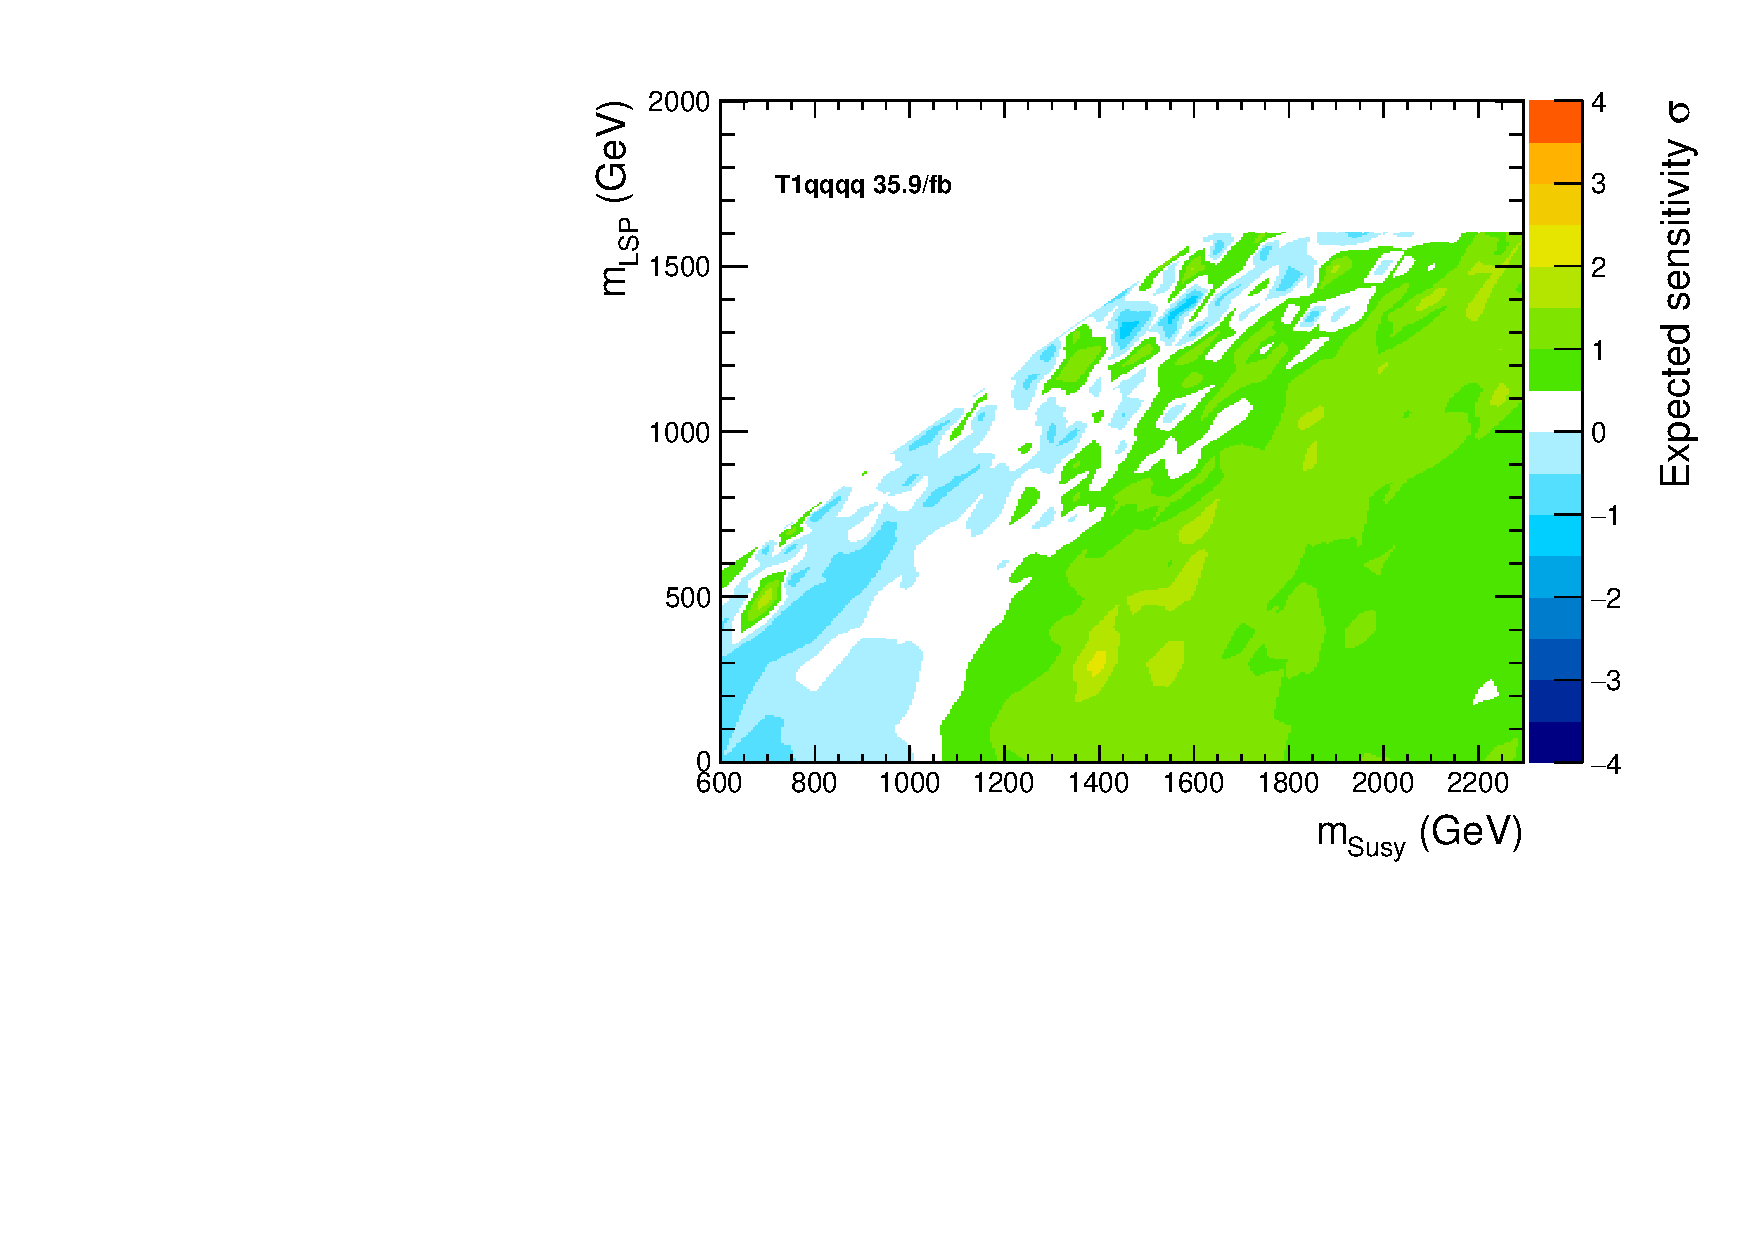
\includegraphics[width=0.45\linewidth]{figures/LLPResults/T1qqqqLL_ctau-1_signif}
        %    \label{fig:T1qqqqLL_signif}
        %} ~~
        \caption{Top: the 95\% C.L. observed upper limit on the cross section
            (histogram), with the expected (solid black line) observed
            (solid red line) exclusion contours. Left: signal acceptance
            including all jet categories. Right: graph showing the four
            most sensitive jet categories for each mass point.
            %Bottom: local observed significance scan.
        }
        \label{fig:T1qqqqLL:ctau-100000}
    \end{center}
\end{figure}
